% ---------------------------------------------------------------------------------------------------------------
% TEMPLATE PARA TRABALHO DE CONCLUSÃO DE CURSO
% Universidade Tecnológica Federal do Paraná - UTFPR
% Customização da classe abnTeX2 (http://www.abntex.net.br/) para as normas da UTFPR
%
% Autores: Diego Marczal
% 	       Michael Vornes <https://github.com/mvornes>
% Adaptação (DACOM-CP): Silvio Ricardo Rodrigues Sanches
%
%----------------------------------------------------------------------------------------------------------------
% Codificação: UTF-8
% LaTeX:  abnTeX2          
% ---------------------------------------------------------------------------------------------------------------


% CARREGA CLASSE PERSONALIZADA DA UTFPR--------------------------------------------------------------------------
\documentclass[%twoside,                   % Impressão em frente e verso
oneside,                   % Impressão apenas frente
]{configuracoes/utfpr-abntex2}


% INCLUI ARQUIVOS DE CONFIGURAÇÕES-------------------------------------------------------------------------------
% REFERÊNCIAS------------------------------------------------------------------
\usepackage[%
    alf,
    abnt-emphasize=bf,
    bibjustif,
    recuo=0cm,
    abnt-url-package=url,       % Utiliza o pacote url
    abnt-refinfo=yes,           % Utiliza o estilo bibliográfico abnt-refinfo
    abnt-etal-cite=3,
    abnt-etal-list=3,
    abnt-thesis-year=final
]{abntex2cite}                  % Configura as citações bibliográficas conforme a norma ABNT

% PACOTES----------------------------------------------------------------------
\usepackage[utf8]{inputenc}                                 % Codificação do documento
\usepackage[T1]{fontenc}                                    % Seleção de código de fonte
\usepackage{booktabs}                                       % Réguas horizontais em tabelas
\usepackage{color, colortbl}                                % Controle das cores
\usepackage{float}                                          % Necessário para tabelas/figuras em ambiente multi-colunas
\usepackage{graphicx}                                       % Inclusão de gráficos e figuras
\usepackage{icomma}                                         % Uso de vírgulas em expressões matemáticas
\usepackage{indentfirst}                                    % Indenta o primeiro parágrafo de cada seção
\usepackage{microtype}                                      % Melhora a justificação do documento
\usepackage{multirow, array}                                % Permite tabelas com múltiplas linhas e colunas
\usepackage{subeqnarray}                                    % Permite subnumeração de equações
\usepackage{lastpage}                                       % Para encontrar última página do documento
\usepackage{verbatim}                                       % Permite apresentar texto tal como escrito no documento, ainda que sejam comandos Latex
\usepackage{amsfonts, amssymb, amsmath}                     % Fontes e símbolos matemáticos
\usepackage[algoruled, portuguese]{algorithm2e}             % Permite escrever algoritmos em português
%\usepackage[scaled]{helvet}                                % Usa a fonte Helvetica
\usepackage{times}                                          % Usa a fonte Times
%\usepackage{palatino}                                      % Usa a fonte Palatino
%\usepackage{lmodern}                                       % Usa a fonte Latin Modern
\usepackage[bottom]{footmisc}                               % Mantém as notas de rodapé sempre na mesma posição
\usepackage{ae, aecompl}                                    % Fontes de alta qualidade
\usepackage{latexsym}                                       % Símbolos matemáticos
\usepackage{lscape}                                         % Permite páginas em modo "paisagem"
%\usepackage{picinpar}                                      % Dispor imagens em parágrafos
%\usepackage{scalefnt}                                      % Permite redimensionar tamanho da fonte
%\usepackage{subfig}                                        % Posicionamento de figuras
%\usepackage{upgreek}                                       % Fonte letras gregas''
\usepackage{ifthen}
\usepackage{listings}


% Redefine a fonte para uma fonte similar a Arial (fonte Helvetica)
\renewcommand*\familydefault{\sfdefault}

% CONFIGURAÇÕES DE APARÊNCIA DO PDF FINAL--------------------------------------
\makeatletter
\hypersetup{%
    portuguese,
    colorlinks=true,   % true: "links" coloridos; false: "links" em caixas de texto
    linkcolor=blue,    % Define cor dos "links" internos
    citecolor=blue,    % Define cor dos "links" para as referências bibliográficas
    filecolor=blue,    % Define cor dos "links" para arquivos
    urlcolor=blue,     % Define a cor dos "hiperlinks"
    breaklinks=true,
    pdftitle={\@title},
    pdfauthor={\@author},
    pdfkeywords={abnt, latex, abntex, abntex2}
}
\makeatother

% ALTERA O ASPECTO DA COR AZUL--------------------------------------------------
\definecolor{blue}{RGB}{41,5,195}

% REDEFINIÇÃO DE LABELS---------------------------------------------------------
\renewcommand{\algorithmautorefname}{Algoritmo}
\def\equationautorefname~#1\null{Equa\c c\~ao~(#1)\null}

% CRIA ÍNDICE REMISSIVO---------------------------------------------------------
\makeindex

% HIFENIZAÇÃO DE PALAVRAS QUE NÃO ESTÃO NO DICIONÁRIO---------------------------
\hyphenation{%
    qua-dros-cha-ve
    Kat-sa-gge-los
}



% INCLUI ARQUIVOS DO TRABALHO DE CONCLUSÃO DE CURSO (PRÉ-TEXTUAIS, TEXTUAIS, PÓS-TEXTUAIS)-----------------------

% INSERE CAPA E FOLHA DE ROSTO
% CAPA---------------------------------------------------------------------------------------------------

% ORIENTAÇÕES GERAIS-------------------------------------------------------------------------------------
% Caso algum dos campos não se aplique ao seu trabalho, como por exemplo,
% se não houve coorientador, apenas deixe vazio.
% Exemplos: 
% \coorientador{}
% \departamento{}

% DADOS DO TRABALHO--------------------------------------------------------------------------------------
\titulo{Geração de Grades Horárias Escolares: Automação com base na meta-heurística Simulated Annealing}
\titleabstract{School Timetable Generation: Simulated Annealing based Generation}
\autor{Allan Wendland Kretzmann}
\autorcitacao{KRETZMANN, Allan} % Sobrenome em maiúsculo
\local{Cornélio Procópio}
\data{2023}

% NATUREZA DO TRABALHO-----------------------------------------------------------------------------------
% Opções: 
% - Trabalho de Conclusão de Curso (se for Graduação)
% - Dissertação (se for Mestrado)
% - Tese (se for Doutorado)
% - Projeto de Qualificação (se for Mestrado ou Doutorado)
\projeto{Trabalho de Conclusão de Curso}

% TÍTULO ACADÊMICO---------------------------------------------------------------------------------------
% Opções:
% - Bacharel ou Tecnólogo (Se a natureza for Trabalho de Conclusão de Curso)
% - Mestre (Se a natureza for Dissertação)
% - Doutor (Se a natureza for Tese)
% - Mestre ou Doutor (Se a natureza for Projeto de Qualificação)
\tituloAcademico{Bacharel em Engenharia de Computação}

% ÁREA DE CONCENTRAÇÃO E LINHA DE PESQUISA---------------------------------------------------------------
% Se a natureza for Trabalho de Conclusão de Curso, deixe ambos os campos vazios
% Se for programa de Pós-graduação, indique a área de concentração e a linha de pesquisa
\areaconcentracao{}
\linhapesquisa{}

% DADOS DA INSTITUIÇÃO-----------------------------------------------------------------------------------
% Se a natureza for Trabalho de Conclusão de Curso, coloque o nome do curso de graduação em "programa"
% Formato para o logo da Instituição: \logoinstituicao{<escala>}{<caminho/nome do arquivo>}
\instituicao{Universidade Tecnológica Federal do Paraná}
\departamento{Departamento Acadêmico de Computação}
\programa{Curso de Engenharia de Computação}
\logoinstituicao{0.2}{dados/figuras/logo-instituicao.png} 

% DADOS DOS ORIENTADORES---------------------------------------------------------------------------------
\orientador{André Yoshiaki Kashiwabara}
%\orientador[Orientadora:]{Nome da orientadora}
\instOrientador{Universidade Tecnológica Federal do Paraná}

%\coorientador{Nome do coorientador}
%\coorientador[Coorientadora:]{Nome da coorientadora}
%\instCoorientador{Instituição do coorientador}

% FOLHA DE ROSTO--------------------------------------------------------------------------------------------------------

% TRABALHO DE CONCLUSÃO DE CURSO
 \preambulo{{\imprimirprojeto} apresentado ao {\imprimirprograma} da {\imprimirinstituicao}, como requisito parcial para a obtenção do título de {\imprimirtituloAcademico}.}

% DISSERTAÇÃO DE MESTRADO
% \preambulo{{\imprimirprojeto} apresentada ao Programa de \mbox{Pós-graduação} da {\imprimirinstituicao}, como requisito parcial para obtenção do título de {\imprimirtituloAcademico}.}

% TESE DE DOUTORADO
% \preambulo{{\imprimirprojeto} apresentada ao Programa de \mbox{Pós-graduação} da {\imprimirinstituicao}, como requisito parcial para a obtenção do título de {\imprimirtituloAcademico}.}

% PROJETO DE QUALIFICAÇÃO DE MESTRADO OU DOUTORADO
%\preambulo{{\imprimirprojeto} apresentado ao Programa de \mbox{Pós-graduação} da {\imprimirinstituicao}, como requisito parcial para a obtenção do título de {\imprimirtituloAcademico}.}

% OBSERVAÇÕES-----------------------------------------------------------------------------------------------------------
% Altere este arquivo APENAS comentando as linhas que não se aplicam ao tipo de trabalho acadêmico desejado.



\begin{document}
	
	\pretextual
	\imprimircapa                                   % Comando para imprimir Capa
	
	
	% \def \license {BY}
	% \def \license {BYSA}
	% \def \license {BYND}
	% \def \license {BYNC}
	% \def \license {BYNCSA}
	\def \license {BYNCND}
	% Define qual licença do trabalho
	
	\imprimirfolhaderosto       
	% Comando para imprimir Folha de rosto
	
	% -----------------------------------------------------------------------------
% Folha de Aprovação
% -----------------------------------------------------------------------------

\textopadraofolhadeaprovacao{Esta folha deverá ser substituída pela cópia digitalizada da folha de aprovação fornecida.}

% -----------------------------------------------------------------------------
% Este documento foi mantido apenas para preservar a paginação do trabalho
% acadêmico final, após a inserção da folha de aprovação fornecida
% -----------------------------------------------------------------------------
 
	
	% INSERE ELEMENTOS PRÉ-TEXTUAIS
	%% DEDICATÓRIA------------------------------------------------------------------

\renewcommand{\dedicatorianame}{DEDICATÓRIA}

\begin{dedicatoria}

Altere este texto inserindo a dedicatória do seu trabalho. 

\end{dedicatoria}
          			   % Dedicatória
	%% AGRADECIMENTOS---------------------------------------------------------------

\begin{agradecimentos}[AGRADECIMENTOS]

Edite e coloque aqui os agradecimentos às pessoas e/ou instituições que contribuíram para a realização do trabalho.

É obrigatório o agradecimento às instituições de fomento à pesquisa que financiaram total ou parcialmente o trabalho, inclusive no que diz respeito à concessão de bolsas.

\end{agradecimentos}
        			   % Agradecimentos
	%% EPÍGRAFE---------------------------------------------------------------------

\renewcommand{\epigraphname}{EPÍGRAFE}

\begin{epigrafe}

\textit{Eu denomino meu campo de Gestão do Conhecimento, mas você não pode gerenciar conhecimento. Ninguém pode. O que pode fazer - o que a empresa pode fazer - é gerenciar o ambiente que otimize o conhecimento. (PRUSAK, Laurence, 1997).}

\end{epigrafe}

% OBSERVAÇÕES------------------------------------------------------------------
% Altere o texto para inserir a epígrafe do seu trabalho
              			   % Epígrafe
	% RESUMO--------------------------------------------------------------------------------

\begin{resumo}[RESUMO]
\begin{SingleSpacing}

% Não altere esta seção do texto--------------------------------------------------------
\imprimirautorcitacao. \imprimirtitulo. \imprimirdata. \pageref {LastPage} f. \imprimirprojeto\ – \imprimirprograma, \imprimirinstituicao. \imprimirlocal, \imprimirdata.\\
%---------------------------------------------------------------------------------------

O \textit{High School Timetabling Problem} consiste na tarefa de alocar aulas a horários letivos em instituições de ensino, considerando restrições relacionadas aos professores, salas e disciplinas. Apesar de todos os avanços tecnológicos que experenciamos na atualidade, esta tarefa ainda é realizada primordialmente de maneira manual nas escolas brasileiras, produzindo grades horárias subótimas e consequentemente trazendo frustrações a todos os envolvidos, sejam estes alunos, docentes ou diretores. Todas as dificuldades relacionadas ao problema, somadas a novos desafios como os Itinerários Formativos do Novo Ensino Médio, pedem uma solução melhor. Este trabalho teve como objetivo implementar um sistema de geração automatizada das grades horárias atendendo o maior número de objetivos possível, através da aplicação de um algoritmo de otimização baseado na meta-heurística \textit{Simulated Annealing}, técnica de otimização inspirada no processo de recozimento de materiais na metalurgia. A solução desenvolvida é uma aplicação \textit{web} que segue uma arquitetura cliente-servidor empregando JavaScript no \textit{frontend} e \textit{backend}, além do otimizador desenvolvido na linguagem C++. Espera-se que a aplicação desenvolvida passe a fazer parte do ferramental de instituições de ensino e auxilie estas a entregar horários escolares que superem os diversos desafios associados e providenciem uma experiência melhor para todos.
\\

\textbf{Palavras-chave}: High School Timetabling Problem. Simulated Annealing. Otimização multiobjetivo.

\end{SingleSpacing}
\end{resumo}

% OBSERVAÇÕES---------------------------------------------------------------------------
% Altere o texto inserindo o Resumo do seu trabalho.
% Escolha de 3 a 5 palavras ou termos que descrevam bem o seu trabalho 
             			   % Resumo em Português
	% ABSTRACT--------------------------------------------------------------------------------

\begin{resumo}[ABSTRACT]
\begin{SingleSpacing}

% Não altere esta seção do texto--------------------------------------------------------
\imprimirautorcitacao. \imprimirtitleabstract. \imprimirdata. \pageref {LastPage} f. \imprimirprojeto\ – \imprimirprograma, \imprimirinstituicao. \imprimirlocal, \imprimirdata.\\
%---------------------------------------------------------------------------------------

The High School Timetabling Problem involves the task of assigning classes to class periods in educational institutions while considering constraints related to teachers, classrooms, and subjects. Despite the technological advancements we experience today, this task is still primarily done manually in brazilian schools, resulting in suboptimal timetables and frustrations for all stakeholders, including students, teachers, and administrators. The difficulties associated with the problem, combined with new challenges provided by the new high school model implemented in the country, call for a better solution. This study has aimed to implement an automated timetabling system that satisfies as many objectives as possible by applying an optimization algorithm based on the Simulated Annealing metaheuristic, a technique inspired by the annealing process in metallurgy. The developed solution is a web application following a client-server architecture, employing JavaScript for both the frontend and backend, in addition to the optimizer implemented in the C++ language. We hope that the developed application becomes part of the toolkit for educational institutions and helps them deliver school timetables that overcome the various associated challenges and provide a better experience for all parties involved.
\\

\textbf{Keywords}: High School Timetabling Problem. Simulated Annealing. Multi-objective optimization.

\end{SingleSpacing}
\end{resumo}

% OBSERVAÇÕES---------------------------------------------------------------------------
% Altere o texto inserindo o Abstract do seu trabalho.
% Escolha de 3 a 5 palavras ou termos que descrevam bem o seu trabalho 
             		           % Resumo em Inglês
	% Lista de Figuras----------------------------------------------------------------

\pdfbookmark[0]{\listfigurename}{lof}
\listoffigures*
\cleardoublepage

% OBSERVAÇÕES---------------------------------------------------------------------
% Este arquivo não precisa de ser alterado, pois a lista é gerada automaticamente.
   % Lista de Figuras
	% LISTA DE QUADROS----------------------------------------------------------------

\renewcommand{\listofquadrosname}{LISTA DE QUADROS}

\pdfbookmark[0]{\listofquadrosname}{loq}
\listofquadros*
\cleardoublepage

% OBSERVAÇÕES---------------------------------------------------------------------
% Este arquivo não necessita de ser editado. A lista é gerada automaticamente.
   % Lista de Quadros
	% LISTA DE TABELAS-------------------------------------------------------------

\pdfbookmark[0]{\listtablename}{lot}
\listoftables*
\cleardoublepage

% OBSERVAÇÕES-------------------------------------------------------------------
% Este arquivo não precisa ser alterado, pois a lista é gerada automaticamente.
         		   % Lista de Tabelas
	%% LISTA DE ABREVIATURAS E SIGLAS----------------------------------------------------------

\begin{siglas}
    \item[ABNT] Associação Brasileira de Normas Técnicas
    \item[DECOM] Departamento de Computação
\end{siglas}

% OBSERVAÇÕES-----------------------------------------------------------------------------
% Altere a lista acima para definir os acrônimos e siglas utilizados neste trabalho
          		   % Lista de Abreviaturas e Siglas
	%% LISTA DE SÍMBOLOS------------------------------------------------------------

\begin{simbolos}
    \item[$ \Gamma $] Letra grega Gama
    \item[$ \lambda $] Comprimento de onda
    \item[$ \in $] Pertence
\end{simbolos}

% OBSERVAÇÕES-------------------------------------------------------------------
% Altere a lista acima para definir os símbolos utilizados no trabalho
        		   % Lista de Símbolos
	% LISTA DE ALGORITMOS----------------------------------------------------------

\newcommand{\algoritmoname}{Algoritmo}
\renewcommand{\listalgorithmcfname}{LISTA DE ALGORITMOS}

\floatname{algocf}{\algoritmoname}
\newlistof{listofalgoritmos}{loa}{\listalgoritmoname}
\newlistentry{algocf}{loa}{0}

\counterwithout{algocf}{chapter}
\renewcommand{\cftalgocfname}{\algoritmoname\space}
\renewcommand*{\cftalgocfaftersnum}{\hfill--\hfill}

\pdfbookmark[0]{\listalgorithmcfname}{loa}
\listofalgorithms
\cleardoublepage

% OBSERVAÇÕES------------------------------------------------------------------
% Este arquivo não precisa ser alterado, pois a lista é gerada automaticamente.
   % Lista de Algoritmos
	% SUMÁRIO----------------------------------------------------------------------

\renewcommand{\contentsname}{SUMÁRIO}

\pdfbookmark[0]{\contentsname}{toc}
\tableofcontents*
\cleardoublepage

% OBSERVAÇÕES-------------------------------------------------------------------
% Este arquivo não precisa ser alterado, pois o sumário é gerado automaticamente.
               			   % Sumário
	
	\textual
	% INSERE ELEMENTOS TEXTUAIS
	% INTRODUÇÃO-------------------------------------------------------------------

\chapter{INTRODUÇÃO}
\label{chap:introducao}

A cada ano letivo, se faz necessária a definição de grades horárias que atendam inúmeros requisitos para o bom funcionamento das mais diversas instituições de ensino. Estas exigências dependem e impactam diretamente os envolvidos, sejam estes professores, alunos, gestores, ou ainda, os responsáveis pelo planejamento dos horários. Os requisitos citados anteriormente podem mudar durante o ano, requerendo constantes atualizações das grades definidas. Esta tarefa, segundo \citeonline{Bardadym}, requer grande esforço quando realizada manualmente, frequentemente resultando em soluções subótimas.

Para o desenvolvimento dos horários escolares, vários critérios devem ser considerados, como o número de aulas de cada professor, salas, turnos, além das restrições associadas a cada professor em particular. A combinação destes fatores para a produção de um horário otimizado é conhecida como \textit{school timetabling problem} \cite{FONSECA2016108}. Para a escrita deste trabalho, foi realizada a leitura de artigos que abordam o tema em questão, deste modo os autores \citeonline{FONSECA2016108}, \citeonline{TAN2021113943} e \citeonline{ABRAMSON} se mostraram imprescindíveis para a sua realização.

Ao decorrer da revisão bibliográfica, foi reafirmada a relevância desta pesquisa e da elaboração de um projeto que solucione o problema, dada a complexidade e recorrência deste. \citeonline{POULSEN} estima que a maioria das instituições de ensino brasileiras efetua essa tarefa de maneira manual, o que implica em atrasos para as escolas, além de desgaste entre os docentes envolvidos nas negociações de restrições. Isto justifica novamente a necessidade de uma solução automatizada que entregue grades otimizadas em um tempo hábil.

Diante deste contexto, fica evidente a necessidade de solucionar o seguinte problema: como automatizar a geração de grades horárias que atendam as diversas demandas das instituições de ensino? Por ser um problema combinatório, consideram-se técnicas viáveis \textit{Simulated Annealing}, Busca Tabu, Algoritmos Genéticos, entre outros \cite{TAN2021113943}.

\section{DELIMITAÇÃO DO TEMA}
\label{sec:antesleiame}

O presente trabalho visa abordar o tema de otimização de grades horárias escolares, tendo em mente especificamente as necessidades de instituições brasileiras de ensino fundamental e médio. 

\section{PROBLEMAS E PREMISSAS}
\label{sec:organizacaoTrabalho}

Como mencionado anteriormente, as instituições de ensino necessitam de constantes atualizações de suas grades horárias. Este processo envolve muitas variáveis, e impacta diretamente alunos, professores e gestores. Devido a esta complexidade, o problema já é conhecido na literatura como \textit{school timetabling problem}, sendo divido nos tipos \textit{exam timetabling}, \textit{course timetabling} e \textit{high school timetabling} \cite{TAN2021113943}. Este trabalho tem como foco esta última variação, que, segundo os mesmos autores, é definido em termos da disponibilidade dos professores, número de salas, número de aulas por professor em cada sala e restrições.

\section{OBJETIVOS}
\subsection{Objetivo Geral}

Desenvolver uma aplicação que automatize e simplifique o processo de criação de grades horárias escolares, otimizando diferentes características de qualidade destas, fazendo com que tais sejam livres de conflitos e atendam a restrições impostas pelas instituições de ensino.

\subsection{Objetivos Específicos}

\begin{enumerate}
	\item Compreender quais são as reais necessidades das escolas quanto ao planejamento de grades horárias;
	\item Implementar métricas de qualidade para os horários, que refletem se as necessidades são atendidas com êxito;
	\item Aplicar um algoritmo de otimização na geração de grades que evite conflitos, atenda restrições de horários dos docentes, minimize a quantidade de janelas nas aulas dos professores, faça agrupamentos formando aulas duplas e evite excessos da mesma aula;
	\item Proporcionar uma experiência do usuário simples e agradável durante o uso da aplicação.
\end{enumerate}

\section{ESTRUTURA ORGANIZACIONAL}

O trabalho em questão está estruturado da seguinte forma: o capítulo \ref{chap:introducao} traz a introdução sobre o tema, uma visão geral sobre a pesquisa e seus objetivos; no capítulo \ref{chap:fundamentacaoTeorica} será desenvolvida a fundamentação teórica, listando todas as fontes de conhecimento consultadas para para o desenvolvimento do projeto; a forma de implementação do projeto, seus materiais e métodos serão discutidos no capítulo \ref{chap:desenvolvimento}; o capítulo \ref{chap:resultados} apresentará os resultados do projeto, e o capítulo \ref{chap:conclusao} trará as considerações finais.

                		           % Introdução
	% REVISÃO DE LITERATURA--------------------------------------------------------

\chapter{REVISÃO DE LITERATURA}
\label{chap:fundamentacaoTeorica}

Este capítulo tem como objetivo explicar o problema de \textit{timetabling} e suas especificidades no caso de grades horárias de ensino médio, assim como a técnica de otimização \textit{Simulated Annealing} e sua aplicação ao problema.

\section{TIMETABLING PROBLEM}
O problema de \textit{timetabling} ou alocação de horários é definido em termos de quatro conjuntos, sendo estes horários, recursos, encontros e restrições. O problema consiste em associar os encontros desejados aos horários, utilizando os recursos disponíveis e minimizando as violações das restrições.

É evidente que existem inúmeras tarefas e indústrias que dependem da alocação de horários, portanto é necessário especializar o problema. Uma das variações deste problema é o \textit{school timetabling problem}, que segundo \citeonline{TAN2021113943} subdivide-se em \textit{exam timetabling}, \textit{course timetabling} e \textit{high school timetabling}. Esta última subdivisão, relacionada a escolas de ensino médio, será o foco deste trabalho.

\subsection{Highschool Timetabling Problem}
No caso específico da alocação de horários para escolas de ensino médio, o problema é definido em termos da disponibilidade dos professores, número de salas, número de aulas por professor em cada sala e restrições. Adequando estas necessidades à formulação do \textit{timetabling problem}, os encontros que desejamos alocar são entre os professores e determinada sala de aula, dados os horários de aula em que a escola opera, visando a utilização dos recursos disponíveis, como salas de aula ou laboratórios, minimizando a violação de restrições associadas aos professores e recursos \cite{TAN2021113943}.

Segundo \citeonline{ABRAMSON}, o problema envolve agendar aulas, professores e salas de aula de tal forma que nenhum professor, turma ou sala de aula seja utilizado mais de uma vez em determinado horário. Situações em que ocorra este agendamento de recursos duplicados serão tratadas como ``conflitos'' neste trabalho.

Levando em consideração a necessidade de agendar diversas aulas evitando conflitos, e o atendimento de restrições variadas, o \textit{highschool timetabling problem} é um problema de otimização multiobjetivo, que segundo \citeonline{Cooper} é da classe NP-completo.

Considerando a natureza complexa do problema, este trabalho propõe desenvolver e analisar a eficiência de um algoritmo de \textit{Simulated Annealing}, assim como implementar uma interface para interação com este.

\section{NOVO ENSINO MÉDIO}
\label{sec:novo_ensino_medio}
O Novo Ensino Médio consiste na atualização das matrizes curriculares das salas desta etapa do sistema educacional (1º, 2º e 3º anos). Formulado através da Lei nº 13.415/2017 \cite{lei13415}, o novo modelo traz ainda mais desafios para a tarefa de organização de grades horárias escolares.

O principal destes novos desafios no contexto da criação de grades horárias é o conceito dos Itinerários Formativos, conjuntos de atividades que os estudantes podem escolher realizar durante o ensino médio, como discplinas, projetos, oficinas, entre outros.

No caso de grandes instituições de ensino, é possível que seja viável oferecer essas atividades optativas através da criação de turmas específicas, entretanto, em escolas de pequeno porte, a adição destas turmas e quantidade relativamente pequena de estudantes por turma pode facilmente desgastar os recursos da instituição.

Tendo estas limitações em mente, observou-se que uma estratégia aplicada por escolas de porte menor é a oferta de disciplinas optativas (Itinerários Formativos) em horários simultâneos em diferentes salas, nos períodos normais de ensino. No momento em que essas aulas acontecem, cada aluno das duas turmas se locomove para a sala adequada onde a aula que escolheu será ministrada, e com isso a escola não precisa alocar salas, professores ou horários adicionais. 

Evidentemente, alocar horários simultâneos para determinadas aulas dificulta ainda mais o planejamento do horário escolar, sendo assim mais uma questão que pode ser auxiliada por um sistema de otimização da grade.

\section{SIMULATED ANNEALING}
Diversos problemas podem ser resolvidos imitando o que ocorre em fenômenos físicos ou naturais. Segundo \citeonline{van_1987}, \textit{Simulated Annealing} é uma meta-heurística que se inspira no processo de recozimento na área da metalurgia. Este processo tem como objetivo reduzir as tensões internas de determinado material, da seguinte forma:

\begin{enumerate}
	\item O material inicia com uma alta temperatura, com seus átomos desordenados e livres para vibrarem e se deslocarem
	\item O sistema é resfriado gradualmente, fazendo com que os átomos encontrem posições cada vez mais estáveis. Em outras palavras, conforme a temperatura diminui, torna-se cada vez mais improvável um átomo se deslocar para uma posição menos estável
	\item Por fim, atinge-se certa temperatura em que não ocorrem mais mudanças significativas no material. 
\end{enumerate}

Esta meta-heurística foi escolhida para o desenvolvimento deste trabalho considerando seu potencial verificado durante a revisão de literatura, e a clareza dos paralelos que podem ser realizados com o processo de têmpera real: os átomos representam os professores e aulas, que podem ser deslocados na grade horária até que atinjam uma posição estável, ou seja, que viole o mínimo possível de restrições do problema.


         % Revisão de Literatura
	%% METODOLOGIA------------------------------------------------------------------

\chapter{PROPOSTA}
\label{chap:proposta}
Neste capítulo será elaborada a proposta de desenvolvimento do projeto, tecnologias e metodologias a serem utilizadas.

\section{PÚBLICO-ALVO}
Identificou-se como público-alvo para o projeto desenvolvido o conjunto de diretores e demais profissionais responsáveis pela elaboração de grades horárias em escolas de ensino fundamental e médio. Quanto à dimensão das instituições de ensino, o trabalho visa contemplar aquelas de pequeno e médio porte.

\section{TECNOLOGIAS E FERRAMENTAS}
Como mencionado anteriormente, o presente trabalho tem como objetivo o desenvolvimento de uma aplicação que automatize e simplifique o processo de criação de grades horárias escolares. Para concluir este objetivo, optou-se por desenvolver uma aplicação que execute no servidor, com uma interface \textit{web} para interação com o usuário. 

Vale ressaltar que inicialmente as premissas do problema e informações encontradas na literatura foram utilizadas para nortear o levantamento de requisitos e o desenvolvimento inicial da aplicação. Estes requisitos serão complementados e ajustados de acordo com os dados coletados de potenciais usuários futuros, conforme o critério metodológico exposto na seção \ref{chap:introducao}.

As tecnologias e ferramentas a serem utilizadas são:

\begin{itemize}
	\item \textbf{VSCode}: Editor de código-fonte desenvolvido pela Microsoft, escolhido por sua versatilidade e aplicabilidade para desenvolver todos os componente do sistema
	\item \textbf{DBeaver}: Ferramenta de código aberto de administração de bancos de dados, utilizada para validação da modelagem e interações manuais com a base de dados
	\item \textbf{PostgreSQL}: Sistema gerenciador de banco de dados relacional, escolhido por sua robustez, possibilitará a persistência dos dados da aplicação em tabelas
	\item \textbf{JavaScript}: Linguagem de programação ubíqua na engenharia de software, escolhida por sua versatilidade para desenvolver a interface \textit{web} e servidor
	\item \textbf{VueJS}: \textit{Framework} para desenvolvimento frontend na linguagem JavaScript, escolhido por sua versatilidade e familiaridade do graduando com este
	\item \textbf{VuetifyJS}: \textit{Framework} de componentes e estilização para o VueJS, utilizado para padronizar o design da aplicação
	\item \textbf{NodeJS}: \textit{Runtime} de JavaScript que permite a utilização dessa linguagem para escrever aplicações no lado do servidor;
	\item \textbf{ExpressJS}: \textit{Framework} para desenvolvimento backend na lignuagem JavaScript, utilizando a plataforma NodeJS
	\item \textbf{C++}: Liguagem de programação compilada, escolhida por sua alta performance para o desenvolvimento do otimizador
	\item \textbf{G++}: Compilador utilizado para converter o código fonte em C++ do otimizador para um arquivo executável 
	\item \textbf{GDB}: Debugador da linguagem C++, utilizado para localizar problemas no código fonte do otimizador
\end{itemize}

\section{ANÁLISE E DESENVOLVIMENTO}
\label{sec:analise_e_desenvolvimento}

\subsection{Interface}
A interface \textit{web} será responsável pela interação do usuário final com a aplicação. Portanto, deverá implementar funcionalidades que possibilitem a configuração das restrições e características das grades horárias a serem geradas, além de mostrar ou exportar tais grades após a geração.

Para o desenvolvimento deste componente, optou-se pelo framework \textit{Vue.js}, devido à riqueza de seu ecossistema de desenvolvimento \textit{frontend} e familiaridade do graduando com este. Complementando este framework, será utilizado também o \textit{Vuetify.js}, a fim de facilitar e padronizar o design da aplicação.

A \autoref{fig:diagrama-uc} mostra os casos de uso que a interface \textit{web} será responsável por disponibilizar:

\begin{figure}[!htb]
	\centering
	\caption{Diagrama de Casos de Uso}
	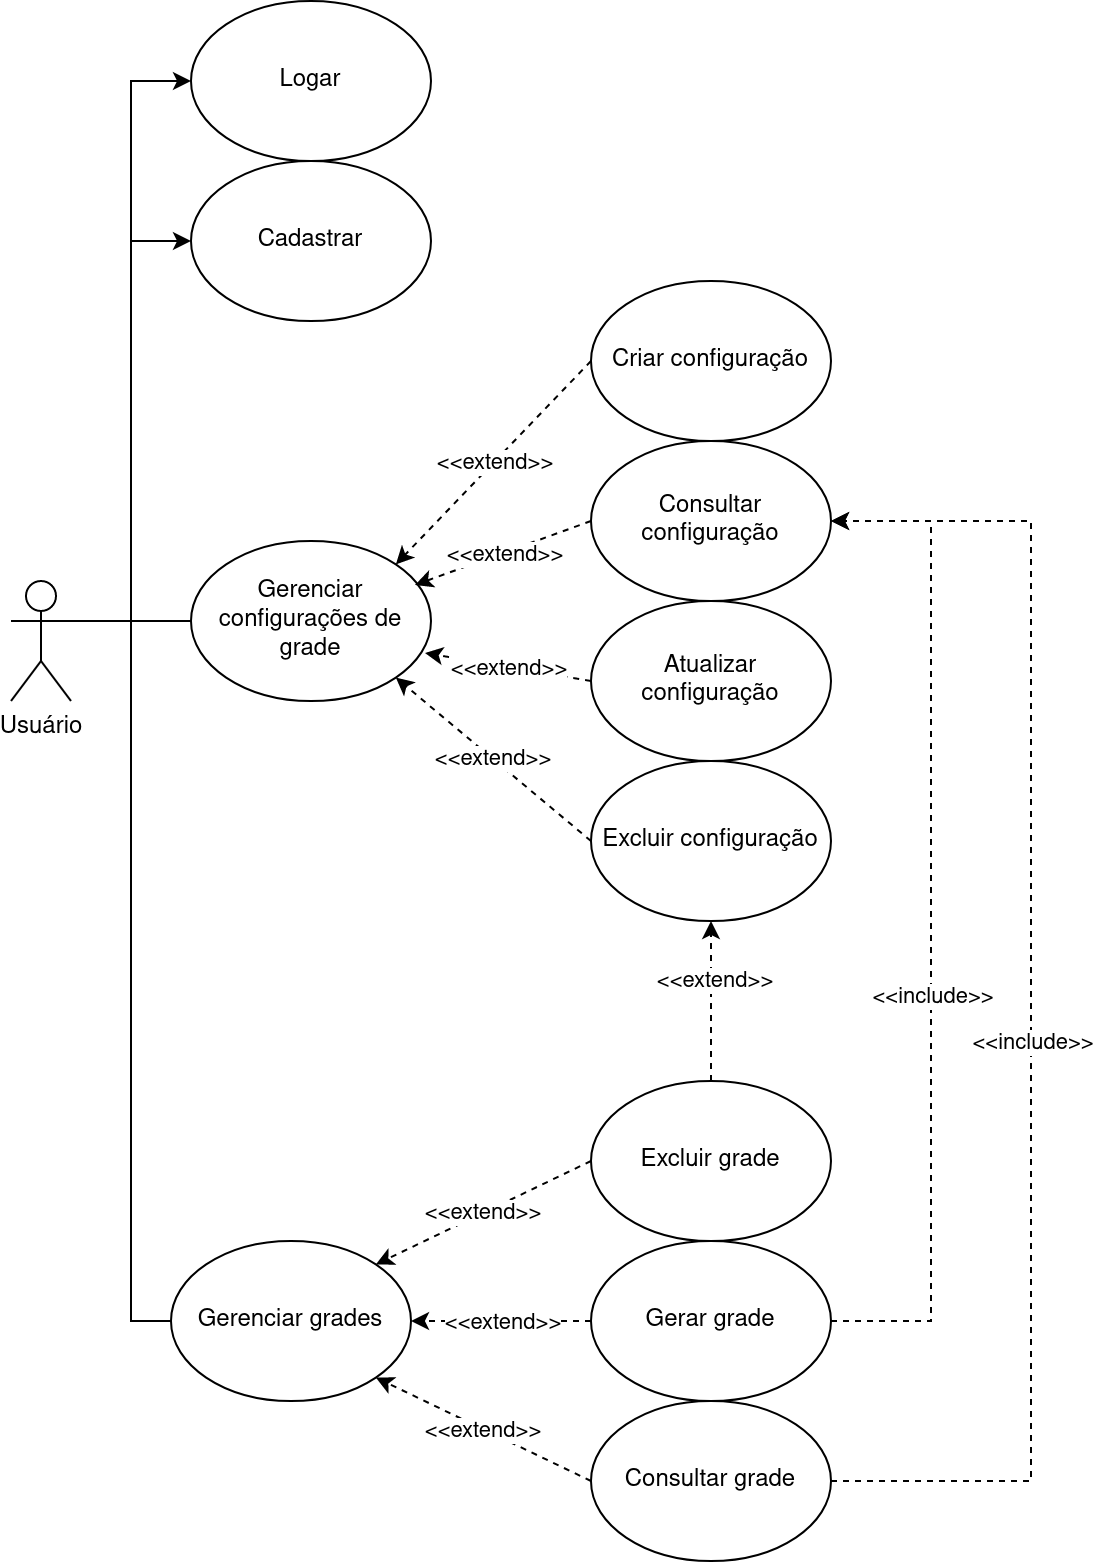
\includegraphics[width=0.65\textwidth]{./dados/figuras/diagrama_uc}
	\fonte{Autor}
	\label{fig:diagrama-uc}
\end{figure}
\newpage

Desenvolveram-se alguns protótipos iniciais das telas necessárias na aplicação.
Primeiramente, a \autoref{fig:tela-configuracoes} mostra a tela de listagem de configurações de grade. Como comentado anteriormente, alguns dos casos de uso da aplicação envolvem o gerenciamento de configurações de grades horárias, as quais são listadas nessa tela.

\begin{figure}[!htb]
	\centering
	\caption{Tela - Listagem de Configurações de Grade}
	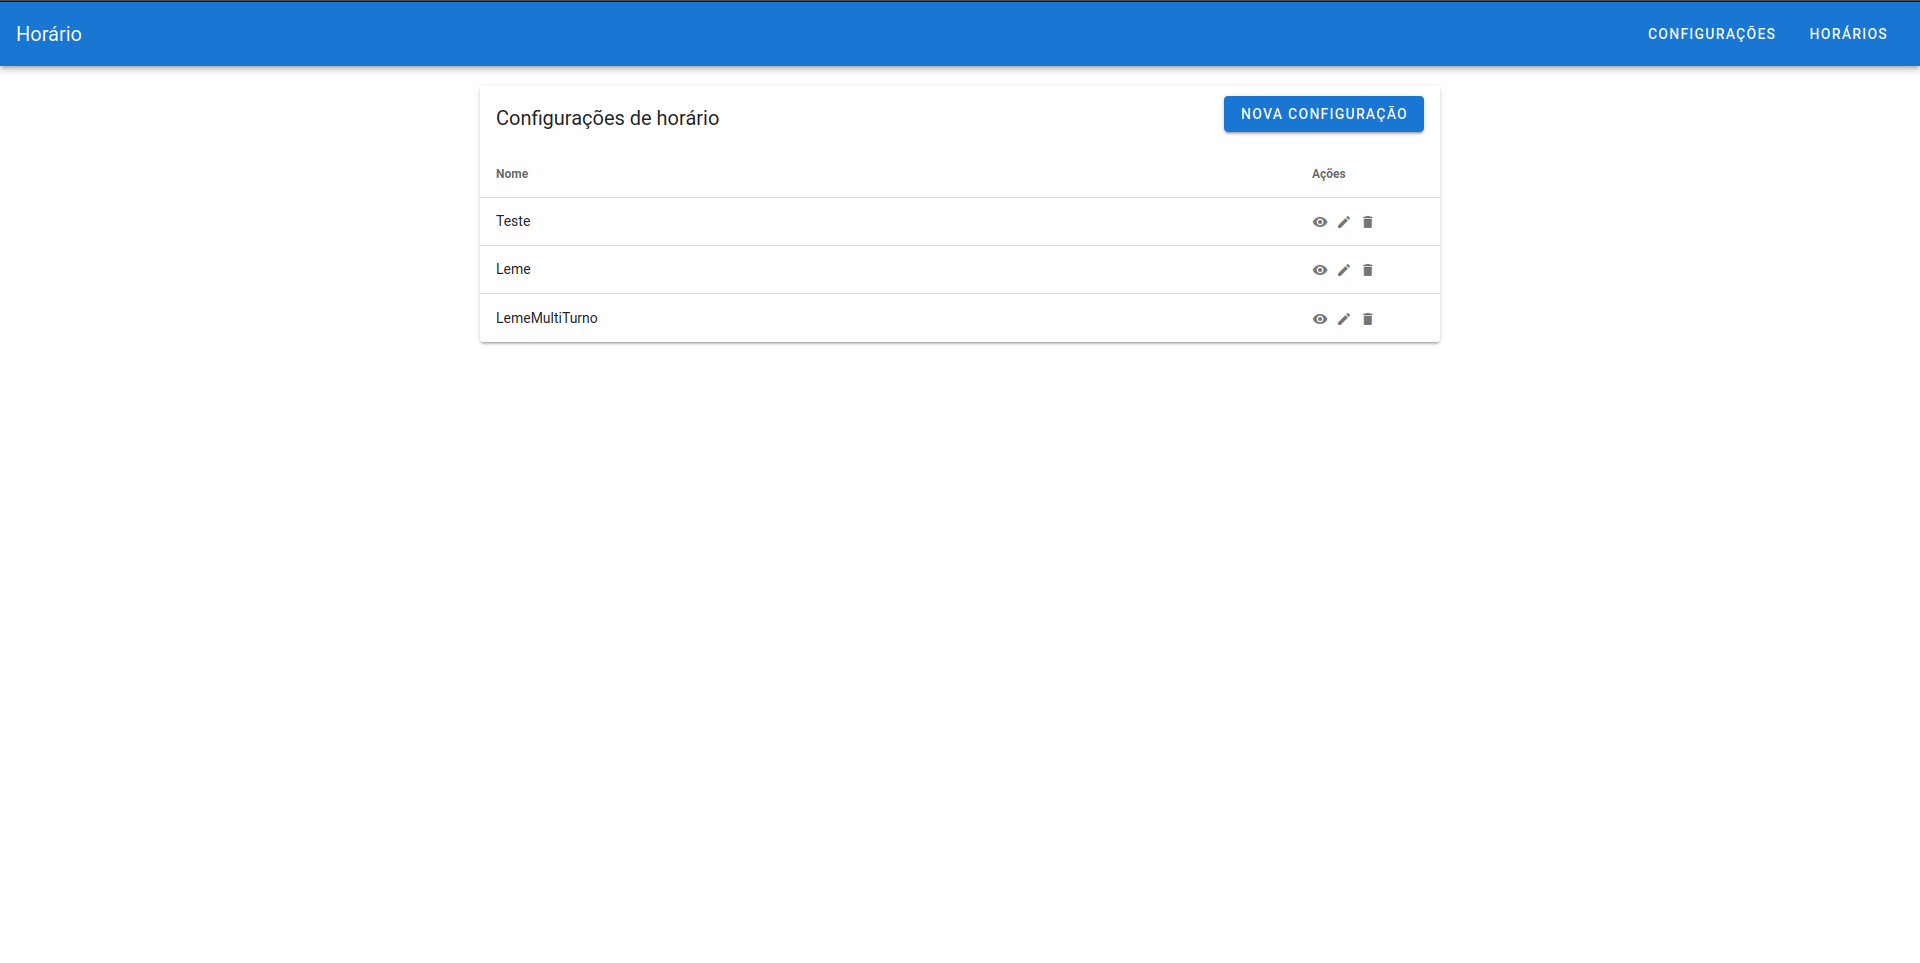
\includegraphics[width=0.8\textwidth]{./dados/figuras/tela_configuracoes}
	\fonte{Autor}
	\label{fig:tela-configuracoes}
\end{figure}

A tela mostrada na \autoref{fig:tela-estrutura1} é responsável por permitir que o usuário cadastre os professores da escola. Nessa tela é possível notar que a aplicação foi estruturada seguindo uma noção de etapas de configuração até a geração da grade horária final. No topo da tela, a etapa "Estrutura da Escola" encontra-se selecionada.

\begin{figure}[!htb]
	\centering
	\caption{Tela - Estrutura da Escola - Professores}
	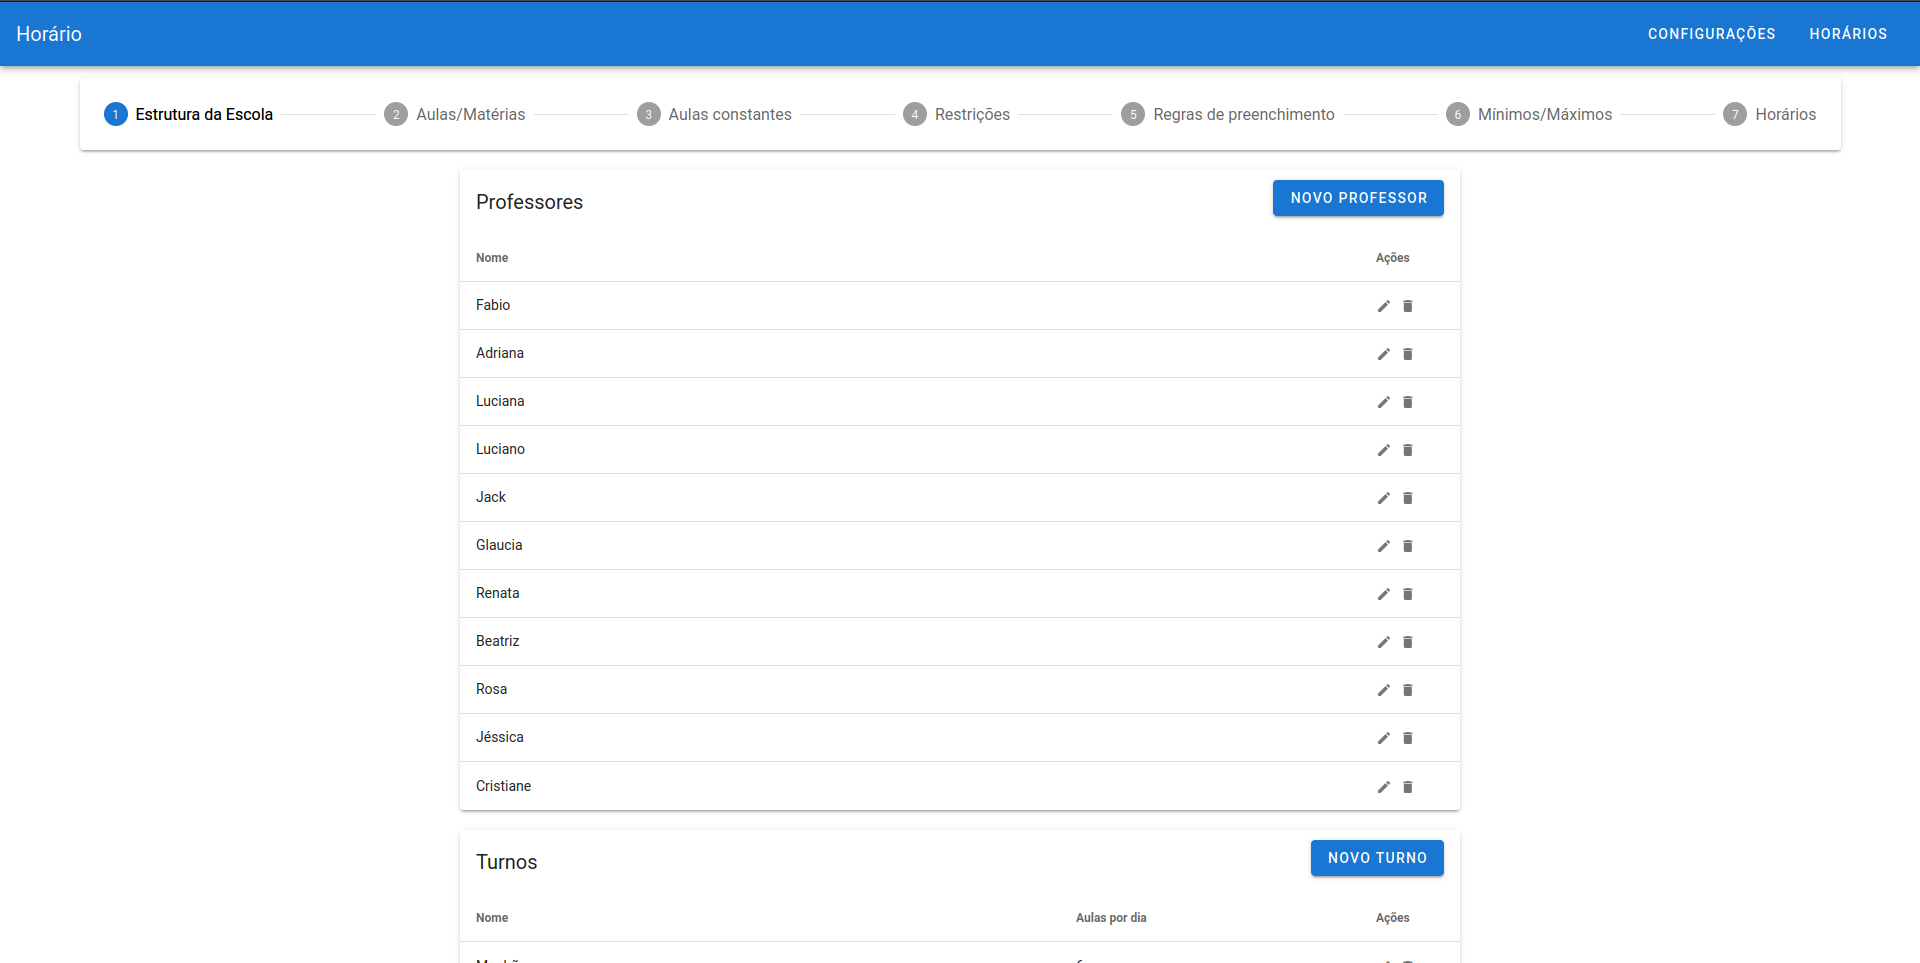
\includegraphics[width=0.8\textwidth]{./dados/figuras/tela_estrutura1}
	\fonte{Autor}
	\label{fig:tela-estrutura1}
\end{figure}
\newpage

Na \autoref{fig:tela-estrutura2}, tem-se a continuação da tela de estrutura da escola, mostrada na \autoref{fig:tela-estrutura1}. Esta parte da tela é responsável pela configuração das salas e turnos da escola.

\begin{figure}[!htb]
	\centering
	\caption{Tela - Estrutura da Escola - Salas e Turnos}
	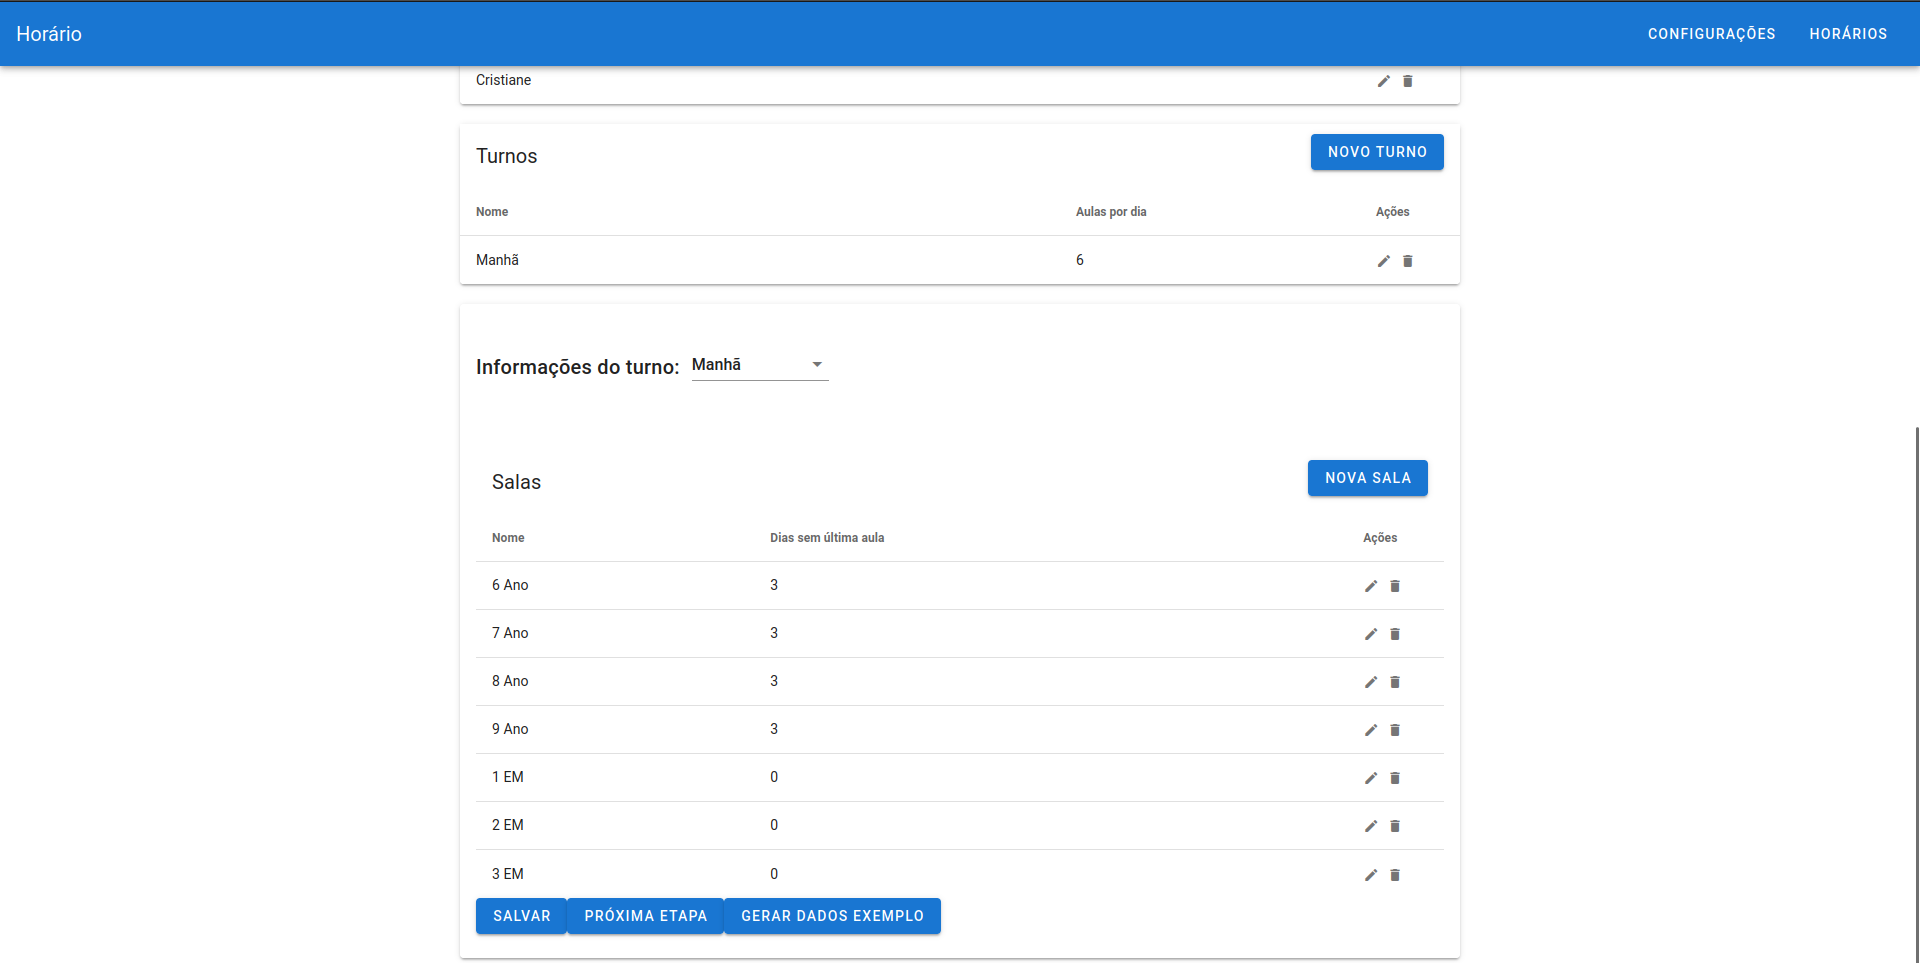
\includegraphics[width=0.8\textwidth]{./dados/figuras/tela_estrutura2}
	\fonte{Autor}
	\label{fig:tela-estrutura2}
\end{figure}

Na tela da \autoref{fig:tela-aulas}, o usuário pode realizar a configuração de número de aulas que cada professor deve ministrar em cada sala, informação fundamental para a geração das grades horárias.

\begin{figure}[!htb]
	\centering
	\caption{Tela - Aulas por professor}
	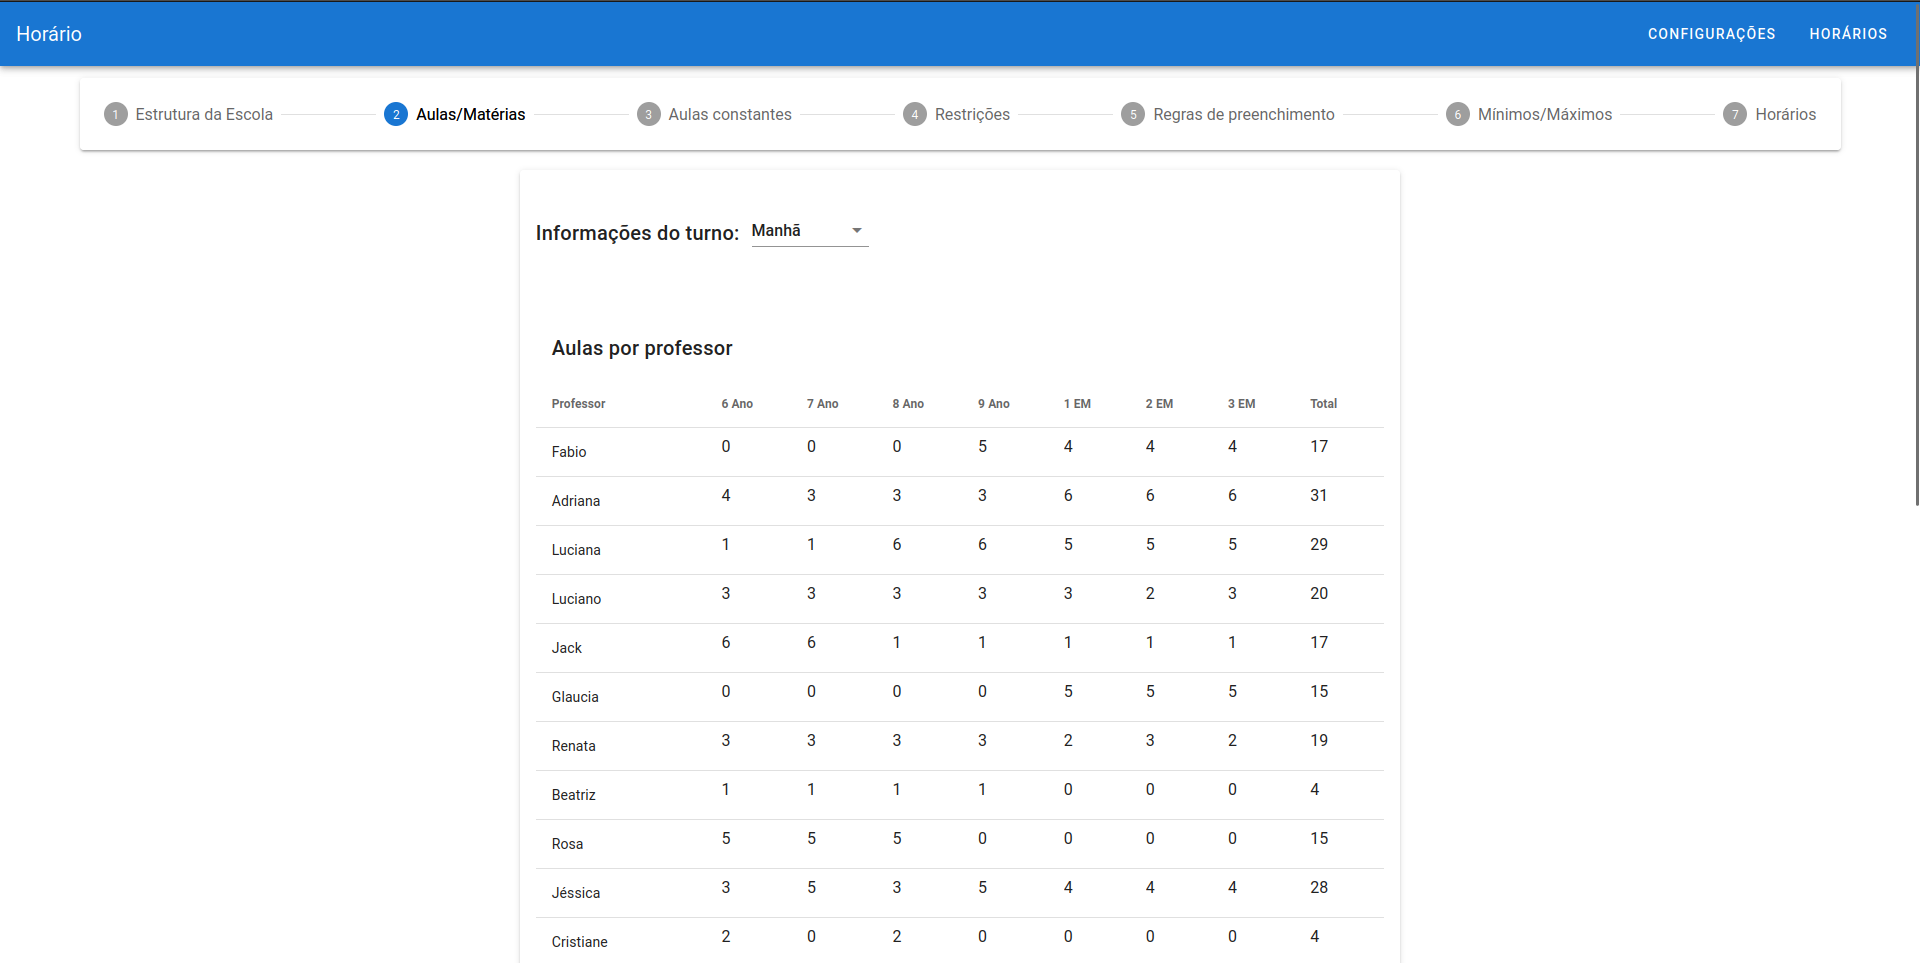
\includegraphics[width=0.8\textwidth]{./dados/figuras/tela_aulas}
	\fonte{Autor}
	\label{fig:tela-aulas}
\end{figure}
\newpage

A tela da \autoref{fig:tela-restricoes} é responsável pela configuração das restrições. Nesta, o usuário pode configurar horários na grade que devem ser evitados ou proibidos para determinado docente.

\begin{figure}[!htb]
	\centering
	\caption{Tela - Restrições}
	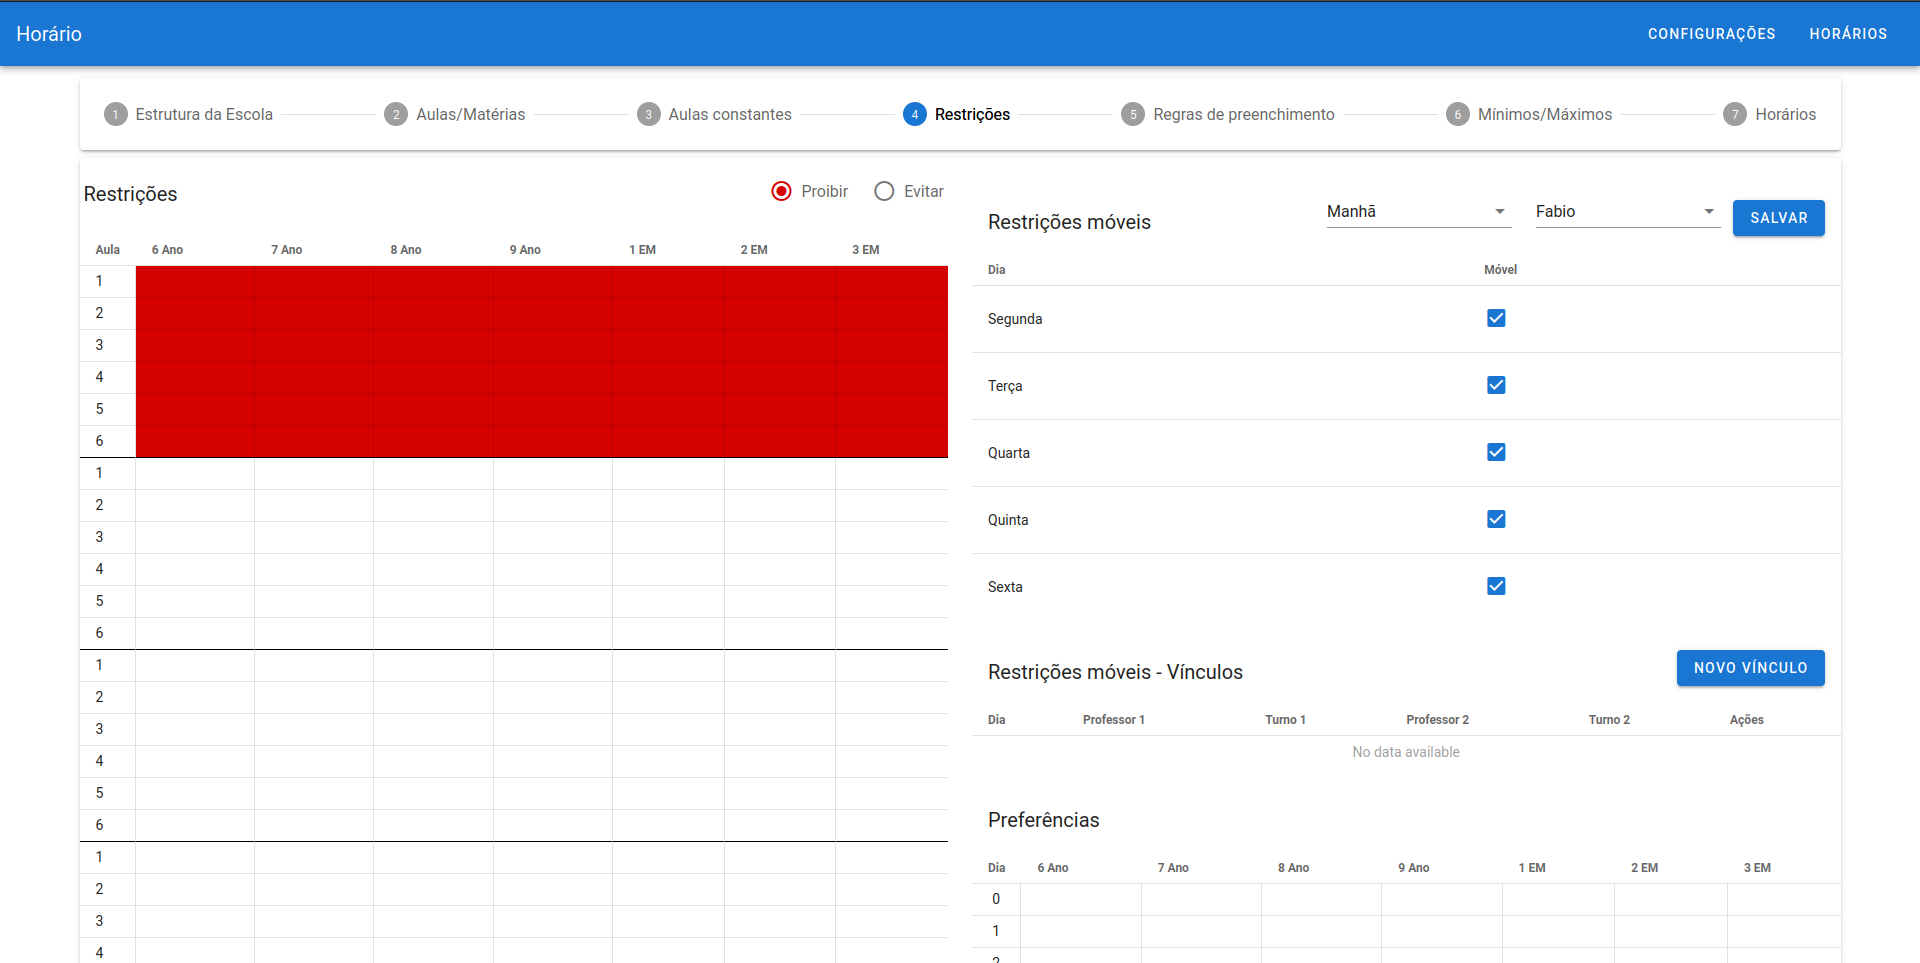
\includegraphics[width=0.8\textwidth]{./dados/figuras/tela_restricoes}
	\fonte{Autor}
	\label{fig:tela-restricoes}
\end{figure}

A última etapa no fluxo da aplicação é representada pela tela da \autoref{fig:tela-horarios}. Nesta, o usuário pode requisitar a geração da grade horária utilizando as configurações realizadas nas etapas anteriores, e acessar as grades geradas anteriormente.

\begin{figure}[!htb]
	\centering
	\caption{Tela - Horários}
	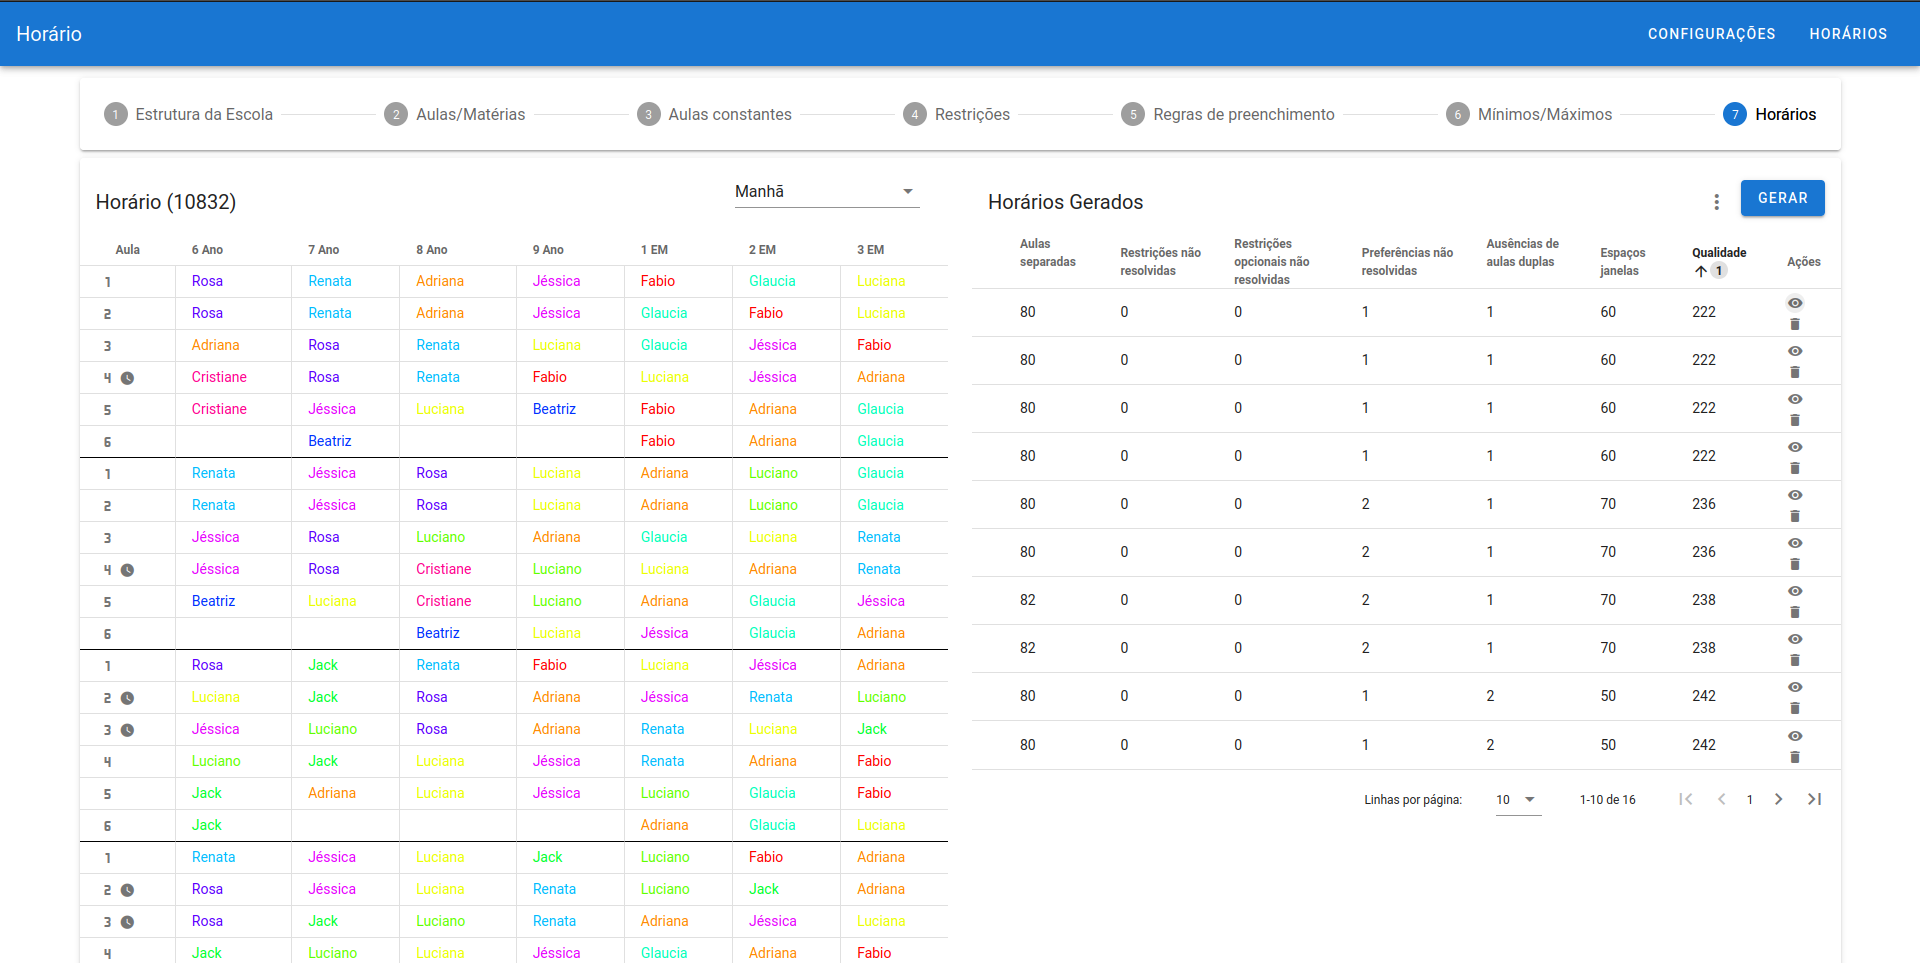
\includegraphics[width=0.8\textwidth]{./dados/figuras/tela_horarios}
	\fonte{Autor}
	\label{fig:tela-horarios}
\end{figure}
\newpage

\subsection{Servidor}
O servidor será responsável por receber as requisições da interface, persistir as configurações no banco de dados e realizar a comunicação com o otimizador, a fim de produzir e armazenar as grades horárias.

Para o desenvolvimento deste componente, optou-se pelo \textit{framework Express.js}, a ser executado na plataforma \textit{Node.js}, devido à simplicidade de implementação que estas tecnologias proporcionam. Em relação ao banco de dados, será utilizado o sistema de gerenciamento de banco de dados \textit{PostgresSQL}, devido à sua robustez.

Conforme as premissas do problema sendo tratado, a modelagem do banco de dados é centrada na entidade ``Configuração'', que agrupa as configurações de determinada instituição de ensino para a geração de suas grades horárias. Cada uma dessas entidades tem turnos, salas, professores, e as configurações de quantas aulas cada professor deve ministrar em cada sala, e as respectivas restrições.

A modelagem comentada está representada na \autoref{fig:diagrama-er}:

\begin{figure}[!htb]
	\centering
	\caption{Modelo Entidade-Relacionamento}
	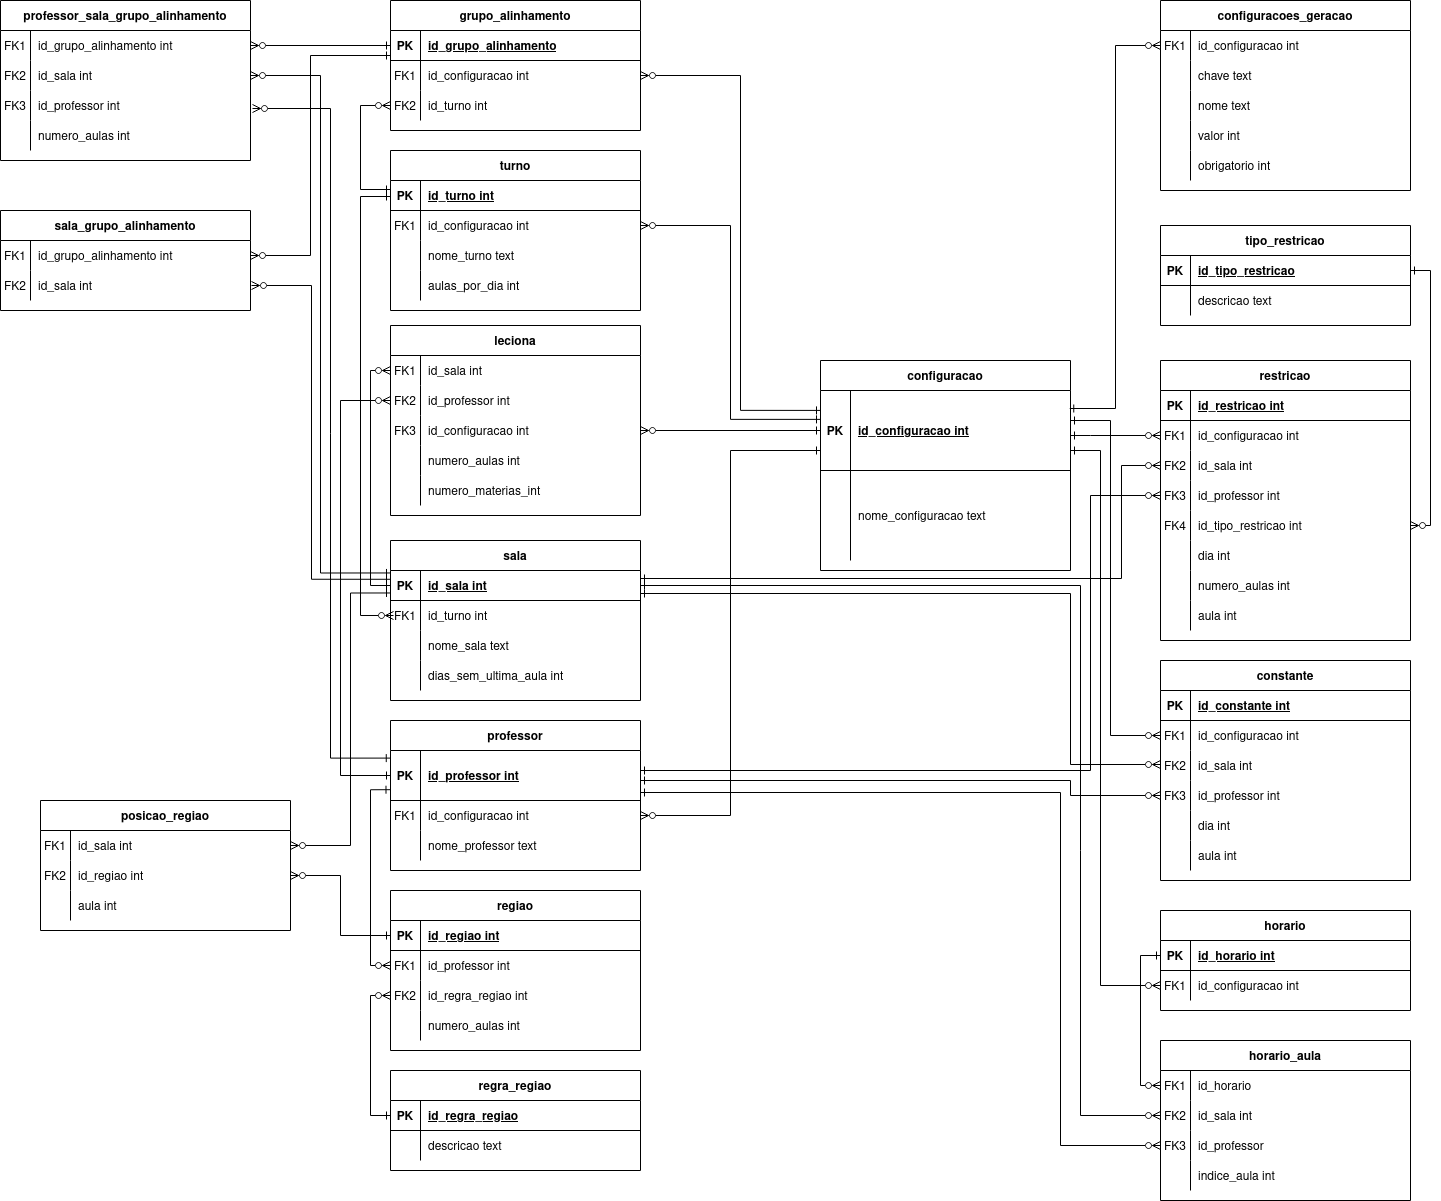
\includegraphics[width=1\textwidth]{./dados/figuras/diagrama_er}
	\fonte{Autor}
	\label{fig:diagrama-er}
\end{figure}
\newpage

Dentre as entidades mostradas no modelo entidade-relacionamento, vale ressaltar a importância da entidade ``Grupo Alinhamento''. Esta será utilizada para configurar aulas que devam acontecer simultaneamente, a fim de resolver o desafio dos itinerários formativos do Novo Ensino Médio, conforme exposto na seção \ref{sec:novo_ensino_medio}.

Para validar a modelagem do banco de dados, realizaram-se inserções de informações de exemplo nas diferentes tabelas. A \autoref{fig:sql-validacao} mostra algumas dessas inserções e os vínculos instituídos pelos identificadores escolhidos.

\begin{figure}[!htb]
	\centering
	\caption{Consultas de validação da modelagem}
	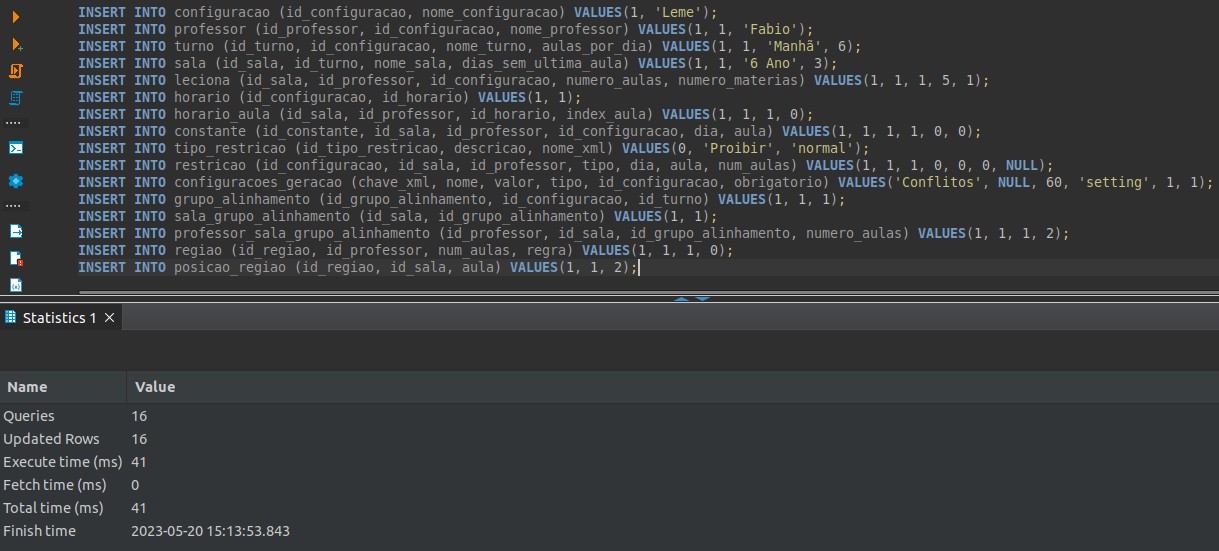
\includegraphics[width=1\textwidth]{./dados/figuras/sql_validacao}
	\fonte{Autor}
	\label{fig:sql-validacao}
\end{figure}
\newpage

Validou-se também o armazenamento das grades horárias no banco de dados. A \autoref{fig:sql-grade} traz um exemplo de consulta de uma grade horária com sete salas:

\begin{figure}[!htb]
	\centering
	\caption{Consulta SQL de grade horária com sete salas}
	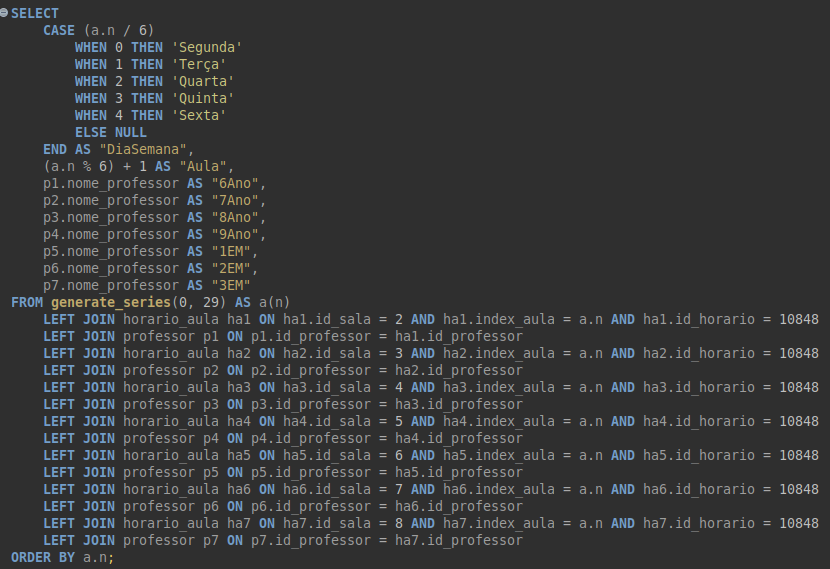
\includegraphics[width=0.7\textwidth]{./dados/figuras/sql_grade}
	\fonte{Autor}
	\label{fig:sql-grade}
\end{figure}

A consulta anterior traz como resultado a tabela visível na \autoref{fig:consulta-grade}, com linhas e colunas correpondentes a horários de aulas e salas respectivamente.

\begin{figure}[!htb]
	\centering
	\caption{Resultado da consulta de uma grade no banco de dados}
	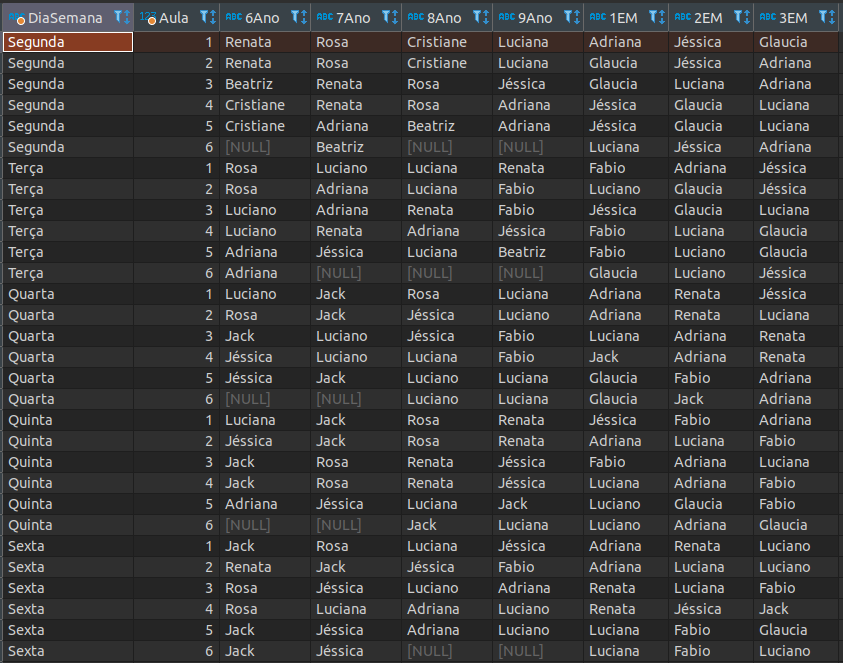
\includegraphics[width=0.7\textwidth]{./dados/figuras/ConsultaGrade}
	\fonte{Autor}
	\label{fig:consulta-grade}
\end{figure}

\newpage
\subsection{Otimizador}
O otimizador será responsável por receber as restrições formatadas pelo servidor, e gerar grades horárias adequadas com base nestas. Após a geração, os resultados devem ser enviados para o servidor para que sejam armazenados no banco de dados.

Este componente do sistema implementará um algoritmo de otimização aplicando a meta-heurística de \textit{Simulated Annealing}, a fim de gerar as soluções para o problema de otimização da grade horária conforme as configurações realizadas pelo usuário.

\section{MÉTODO}
\label{sec:metodo}
Para a processo de software da aplicação, optou-se pelo processo de desenvolvimento incremental. Este processo consiste na divisão da implementação do projeto em incrementos, os quais são executados linearmente, porém de forma escalonada.\cite{pressman2016}

Este processo de software foi escolhido por possibilitar o planejamento de execução do projeto em etapas lógicas, que podem ser sobrepor através de escalonamento, de acordo com as necessidade encontradas. Conforme os requisitos levantados na seção anterior, dividiram-se as tarefas de desenvolvimento nos incrementos pertinentes:
\begin{itemize}
	\item \textbf{Incremento 1}: Desenvolvimento inicial do otimizador, aplicando Simulated Annealing apenas para a resolução de conflitos;
	\item \textbf{Incremento 2}: Implementação de restrições no otimizador;
	\item \textbf{Incremento 3}: Criação do servidor e banco de dados;
	\item \textbf{Incremento 4}: Desenvolvimento da interface \textit{web};
	\item \textbf{Incremento 5}: Adição do sistema de usuários;
	\item \textbf{Incremento 6}: Adaptação da modelagem para incluir matérias aos horários alocados pelo otimizador;
	\item \textbf{Incremento 7}: Implementação de validações das configurações de grade inseridas pelo usuário;
	\item \textbf{Incremento 8}: Desenvolvimento de sistema de exportação de grades horárias.
\end{itemize}

Conforme evidenciado na seção \ref{sec:analise_e_desenvolvimento}, os quatro primeiros incrementos já foram executados, a fim de prototipar o sistema e verificar a viabilidade a solução planejada.

Quanto à validação do software desenvolvido, esta será realizada através de experimentos controlados, simulando requisitos das grades horárias. Após esta etapa, serão conduzidas validações no contexto de instituições de ensino reais que sejam pertinentes ao trabalho.
                   % Proposta
	%% METODOLOGIA------------------------------------------------------------------

\chapter{CRONOGRAMA}
\label{chap:cronograma}
Neste capítulo serão detalhadas as atividades que devem ser executadas até a conclusão deste trabalho, assim como os períodos planejados para a respectiva execução destas.

As tarefas planejadas são a coleta e análise de dados, a fim de verificar a necessidade de adicionar novos tipos de restrições e parametrizações ao otimizador; a execução dos incrementos do software conforme exposto na seção \ref{sec:metodo} e a etapa de validação. Os períodos planejados para cada uma destas atividades constam na \autoref{fig:cronograma}:

\begin{figure}[!htb]
	\centering
	\caption{Cronograma}
	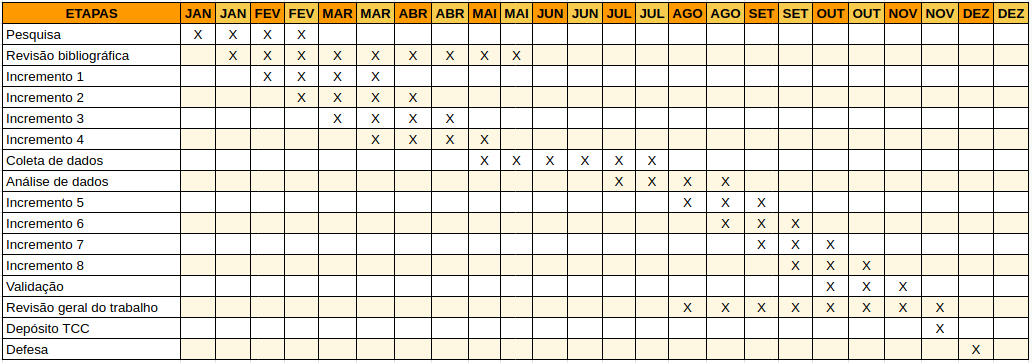
\includegraphics[width=1\textwidth]{./dados/figuras/cronograma}
	\fonte{Autor}
	\label{fig:cronograma}
\end{figure}

	% METODOLOGIA------------------------------------------------------------------

\chapter{DESENVOLVIMENTO}
\label{chap:desenvolvimento}
Este capítulo tem como objetivo evidenciar todas as atividades executadas durante o desenvolvimento do projeto. A \autoref{sec:recursos} apresentará uma listagem dos \textit{softwares} utilizados no desenvolvimento do projeto; a \autoref{sec:metodos} explicitará o método de desenvolvimento, e a \autoref{sec:implementacao} evidenciará a execução das atividades propriamente ditas.

\section{RECURSOS UTILIZADOS}
\label{sec:recursos}

\section{MÉTODOS}
\label{sec:metodos}

\section{ANÁLISE E IMPLEMENTAÇÃO}
\label{sec:implementacao}

\subsection{Otimizador inicial}

Segundo \citeonline{ABRAMSON}, uma parte fundamental para a produção de grades horárias escolares é a resolução de conflitos de recursos. Estes conflitos são caracterizados por recursos alocados simultâneamente, levando a grades horárias não aplicáveis na prática. Um exemplo disso é a alocação de um professor para ministrar aulas para mais de uma turma ao mesmo tempo, o que é impossível.

Neste projeto, a primeira parte desenvolvida foi a versão inicial do otimizador, cuja tarefa era gerar uma grade horária válida, evitando conflitos, ou seja, professores alocados para mais uma turma ao mesmo tempo. O algoritmo \ref{alg:otimizadorInicial} representa esta primeira versão do otimizador, cuja implementação foi baseada no algoritmo genérico de \textit{Simulated Annealing} proposto por \citeonline{van_1987}, visível na figura \ref{fig:procedure}.

\begin{algorithm}
	\caption{Otimizador de grades inicial}
	\label{alg:otimizadorInicial}
	\KwIn{Lista de professores $LP$, lista de turmas $LT$, matriz de aulas por professor por turma $MA$, temperatura inicial $TI$, Taxa de resfriamento $TR$}
	\KwOut{Grade horária de professores otimizada}
	$temperatura \leftarrow TI$\\
	$grade \leftarrow$ CriaGradeInicial$(LP, LT, MA)$\\
	$minConflitos \leftarrow$ NumeroConflitos$(grade)$\\
	\While {condição de parada não atingida} {
		\For {$passo = 0$ até $numeroPassos$} {
			$turma \leftarrow EscolheTurmaAleatoria()$\\
			$linhas \leftarrow EscolheHorariosAleatoriosValidos(turma)$\\
			$delta \leftarrow CalculaDelta(turma, linhas)$\\
			$probabilidade \leftarrow e^{-delta/temperatura}$\\
			$valorAceite \leftarrow Aleatorio(0, 1)$\\
			\If {$delta < 0$ ou $probabilidade \ge valorAceite$} {
				$PermutaProfessores(turma, linha1, linha2)$\\
				\If {NumeroConflitos$(grade)$ < $minConflitos$ } {
					Imprime$(grade)$\\
					$minConflitos \leftarrow$ NumeroConflitos$(grade)$
				}
			}
		}
		$temperatura \leftarrow temperatura * TR$
	}
\end{algorithm}

\begin{figure}[h]
	\centering
	\caption{Algoritmo genérico de Simulated Annealing}
	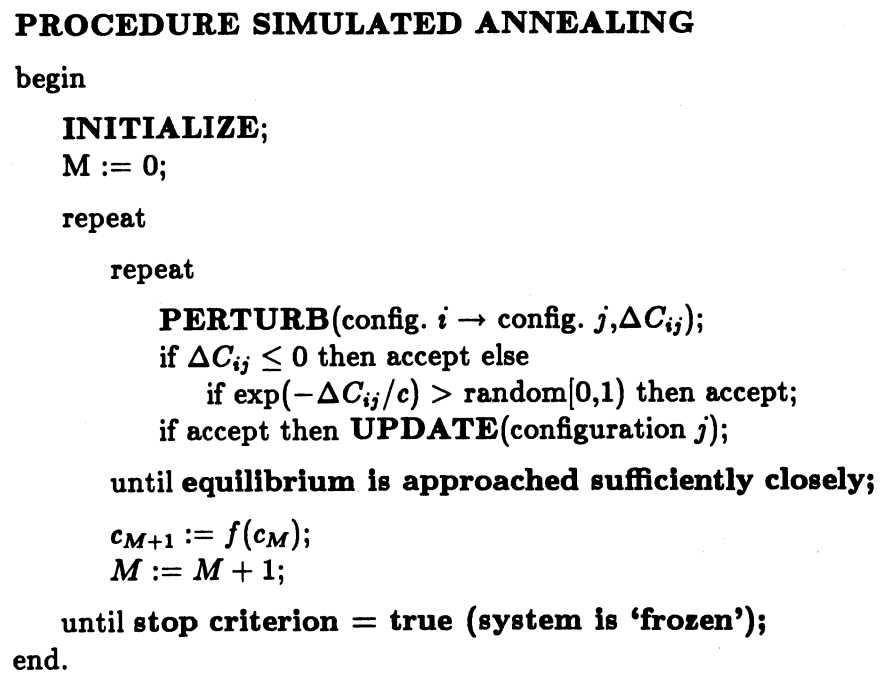
\includegraphics[width=1\textwidth]{./dados/figuras/procedure_simulated_annealing}
	\fonte{Figura 2.1 de \citeonline{van_1987}}
	\label{fig:procedure}
\end{figure}

No algoritmo \ref{alg:otimizadorInicial}, o valor da taxa de resfriamento é de 0,99, sendo a temperatura inicial e o número de passos por iteração escolhidos empiricamente. Sobre a temperatura inicial, esta deve receber um valor suficientemente alto para que possibilite as diversas trocas de posições da grade horária para a geração de uma solução satisfatória, mas não tão alto a ponto de fazer o algoritmo passar boa parte do tempo de execução realizando trocas aleatórias. Este valor 
pode ser definido empiricamente, ou utilizando o método explicitado por \citeonline{abramsomCooling}, em que é calculada a temperatura em que as soluções passam por uma transição de fase.

Explicando melhor o algoritmo, o método ``CriaGradeInicial''  gera uma matriz com as turmas e números de aulas de cada professor alocados corretamente. Esta grade inicial provavelmente possui inúmeros conflitos, portanto são aplicados os passos de otimização. Para cada passo de otimização, são escolhidas aleatoriamente uma turma e duas linhas (posições) da grade horária. Com estas informações, é calculada a variação do número de conflitos que a permutação dos professores nas linhas escolhidas ocasionaria. 

De acordo com o valor de variação calculado (delta), é determinado se a troca dos professores deve ou não ser realizada: uma troca que diminua o número de conflitos sempre é aceita, enquanto uma troca que aumenta o número de conflitos pode ser aceita probabilistacamente, de acordo com o valor da temperatura na iteração atual.

Em relação à condição de parada, durante o desenvolvimento deste primeiro incremento optou-se por utilizar o esgotamento da temperatura, ou seja, o algoritmo finaliza sua execução assim que a temperatura atinge um valor próximo de zero, quando não ocorrem mais permutações de professores.



\subsection{PESOS E RESTRIÇÕES}
\label{subsec:pesos_e_restricoes}

Apesar da importância da resolução de conflitos, existem diversas outras nuances durante o planejamento das grades horárias que precisam ser levadas em conta para que as grades produzidas sejam aplicáveis na prática.

\citeonline{ABRAMSON} sugere uma forma de permitir a otimização de múltiplas características simultanemente utilizando: uma função de custo ponderado. Esta função foi implementada, utilizando-se um sistema de métricas, cada qual mensura quantitativamente determinada característica da grade horária, e contém um peso que define a sua importância para a grade como um todo. 

A função de custo ponderado retorna um valor que representa a qualidade geral de uma grade horária, através do cálculo da média ponderada de todas as métricas de qualidade. Em outras palavras, quanto menor o custo, melhor a solução encontrada.

Adicionalmente, as métricas foram implementadas de forma que pudessem ser rígidas ou suaves. As métricas rígidas precisam ser perfeitamente atendidas para que a grade horária seja considerada viável, enquanto as métricas suaves promovem a melhoria da qualidade, mas não necessariamente precisam ser perfeitamente atendidas.

As próximas seções terão como objetivo explicar cada uma destas métricas e os desafios associados. A \autoref{subsec:salvamento} entrará em mais detalhes sobre como as grades horárias passaram a ser salvas após a implementação das métricas.

\subsubsection{Agrupamento de aulas}

Observando grades horárias escolares existentes, é possível notar que existe uma motivação para realizar agrupamentos, formando aulas duplas. Isso aumenta a produtividade das aulas, à medida que diminui trocas e deslocamento de professores entre as salas. Para produzir estes agrupamentos, foram adicionadas algumas métricas que fazem o otimizador penalizar:

\begin{enumerate}
	\item Aulas separadas;
	\item Aulas desagrupadas;
	\item Excessos de aulas iguais para determinada turma em um dia;
	\item Dias com todas aulas planejadas distintas para deteriminada turma;
\end{enumerate}

Para contextualizar estas situações, a seguir serão apresentados alguns quadros.

\begin{quadro}[!htb]
	\centering
	\caption{Exemplo de dia com aulas separadas.\label{qua:aulasSeparadas}}
	\begin{tabular}{|p{3cm}|p{3cm}|p{3cm}|}
		\hline
		\textbf{Aula} & \textbf{Professor} & \textbf{Matéria} \\
		\hline
		1 & Marcos & Matemática \\
		\hline
		2 & Fábio & Física \\
		\hline
		3 & Marcos & Matemática \\
		\hline
		4 & Luciana & Português \\
		\hline
		5 & Luciana & Português \\
		\hline
		6 & Luciana & Português \\
		\hline
	\end{tabular}
	\fonte{Autoria própria}
\end{quadro}
\pagebreak

Observando o quadro \ref{qua:aulasSeparadas}, é possível notar:

\begin{itemize}
	\item Aulas separadas: 1, 2 e 3, visto que não estão em nenhum agrupamento;
	\item Aulas desagrupadas: 1 e 3, pois consistem em múltiplas aulas iguais, no mesmo dia, que não foram agrupadas;
	\item Excessos de aulas: 4, 5, 6, pois consiste em uma aula tripla, algo considerado não desejável neste trabalho
\end{itemize}

Por fim, a situação de dias com todas aulas diferentes, que serão referidos como "Dias fragmentados" neste trabalho, pode ser observada no quadro \ref{qua:fragmentado}.

\begin{quadro}[!htb]
	\centering
	\caption{Exemplo de dia fragmentado.\label{qua:fragmentado}}
	\begin{tabular}{|p{3cm}|p{3cm}|p{3cm}|}
		\hline
		\textbf{Aula} & \textbf{Professor} & \textbf{Matéria} \\
		\hline
		1 & Marcos & Matemática \\
		\hline
		2 & Fábio & Física \\
		\hline
		3 & Luciana & Português \\
		\hline
		4 & Roberto & Geografia \\
		\hline
		5 & Renato & História \\
		\hline
	\end{tabular}
	\fonte{Autoria própria}
\end{quadro}

\subsubsection{Constantes}

Durante o desenvolvimento, concebeu-se o conceito de ``Aulas constantes'', como aulas que absolutamente devem ser alocadas em determinada posição da grade horária. Isto é útil para guiar o otimizador rumo a uma solução desejada, quando já são conhecidas algumas aulas que devem ser fixas. 

Como exemplo de caso de uso, uma escola com seis aulas diárias pode ter alguns dias da semana com menos aulas, e pode ser interessante definir explicitamente quais dias devem ter a última aula da grade horária não alocada (vazia). A figura \ref{fig:constantes} mostra um exemplo de configuração de aulas constantes para determinada grade horária.

\begin{figure}[!htb]
	\centering
	\caption{Aulas constantes}
	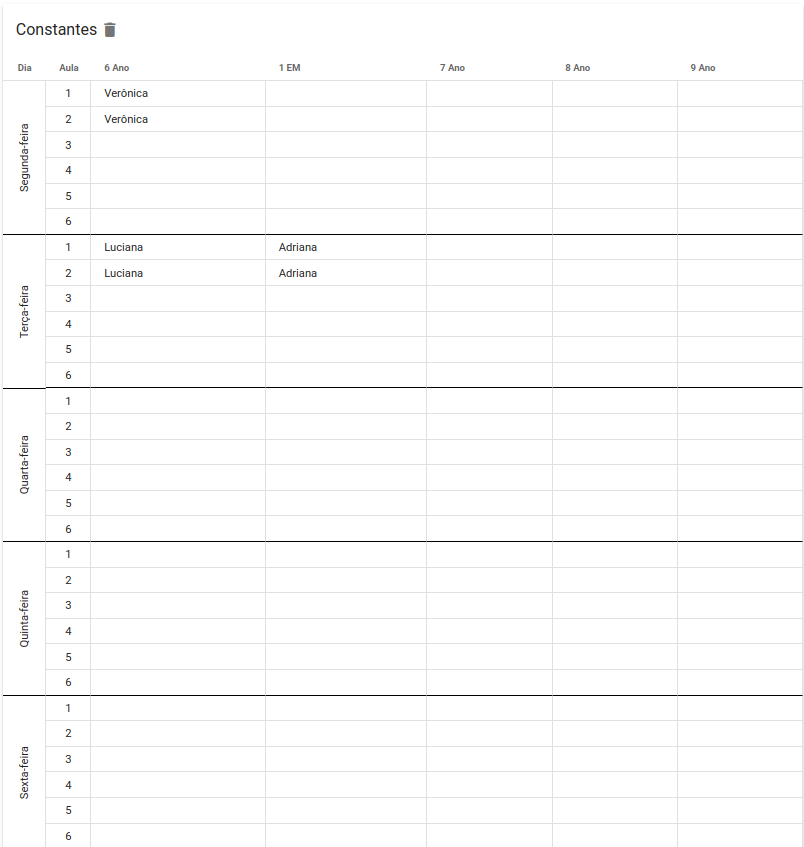
\includegraphics[width=1\textwidth]{./dados/figuras/constantes}
	\fonte{Autor}
	\label{fig:constantes}
\end{figure}
\pagebreak

Considerando a natureza absoluta das aulas constantes, estas não são consideradas um métrica de qualidade, e não possuem um peso próprio. Em vez disso, no método ``GeraGradeInicial'' do algoritmo \ref{alg:otimizadorInicial}, o otimizador já aloca as aulas constantes nas posições desejadas, e a função ``EscolheHorariosAleatoriosValidos'' não seleciona posições que estejam alocadas com aulas constantes. Desta forma, um vez que as aulas constantes são posicionadas na grade horária, estas nunca são movidas durante os passos de otimização.

\subsubsection{Restrições}

As restrições representam o oposto das aulas constantes: posições em que determinadas aulas não devem ser alocadas. Implementaram-se no otimizador restrições suaves e rígidas, cada uma podendo também receber um peso customizado. Dessa forma, é possível configurar o otimizador para nunca alocar determinada aula em certa posição da grade, ou apenas evitar isso.

Como exemplo de uso dessa funcionalidade, a figura \ref{fig:restricoes} demonstra uma configuração de restrições para determinado professor que não pode ser alocado nas duas últimas aulas de qualquer dia da grade horária.

\begin{figure}[!htb]
	\centering
	\caption{Restrições}
	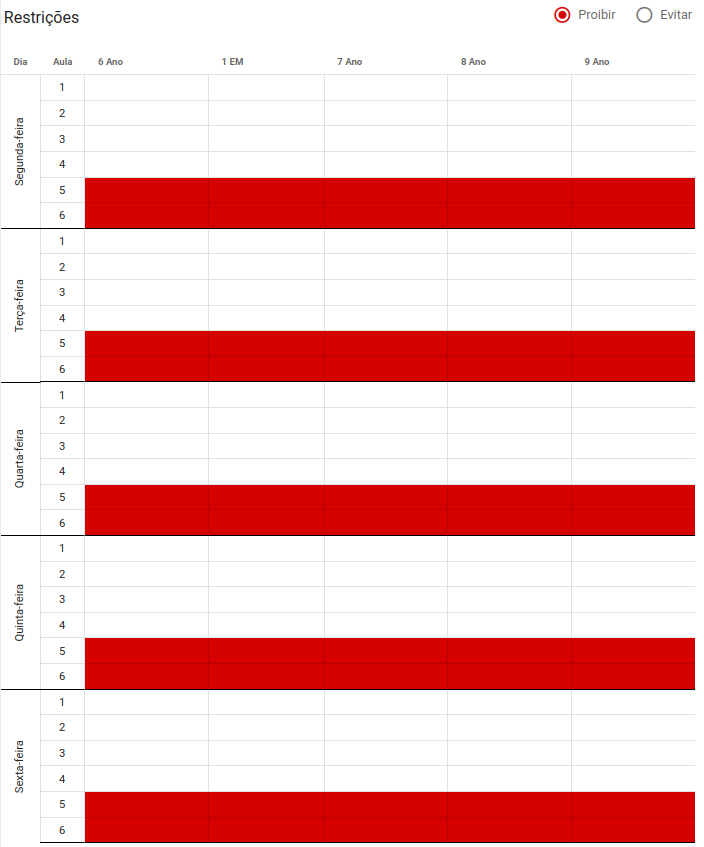
\includegraphics[width=1\textwidth]{./dados/figuras/restricoes}
	\fonte{Autor}
	\label{fig:restricoes}
\end{figure}
\pagebreak

No caso das restrições, a métrica associada mensura a quantidade de restrições violadas, ou seja, posições em que determinada aula foi alocada, mas não deveria ter sido.

\subsubsection{Regiões}

O conceito de regiões foi concebido como uma forma de proporcionar ainda mais controle ao usuário, sobre o posicionamento das aulas na grade horária. Cada região consiste em um grupo arbitrário de posições da grade horária, associado a uma regra relacionada a uma quantidade de aulas. Com as regiões, é possível determinar mínimos, máximos ou quantidades exatas de aulas que devem ser alocadas em certas posições da grade horária.

Como exemplo de uso das regiões, a figura \ref{fig:regioes} demonstra uma configuração utilizada para assegurar que em todos os dias da grade horária, o professor tenha alguma aula alocada no primeiro horário.

\begin{figure}[!htb]
	\centering
	\caption{Exemplo de região}
	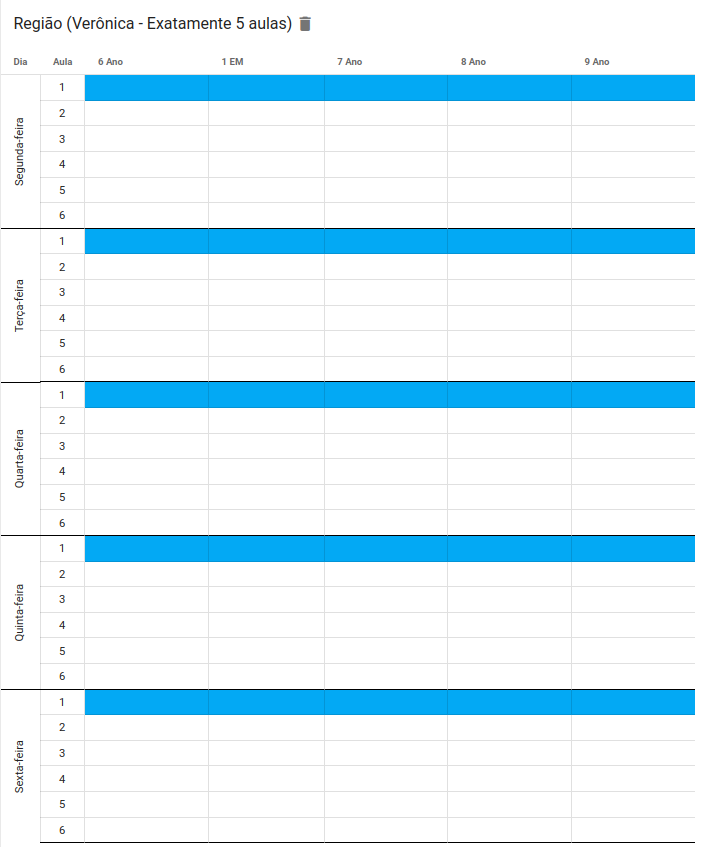
\includegraphics[width=1\textwidth]{./dados/figuras/regioes}
	\fonte{Autor}
	\label{fig:regioes}
\end{figure}
\pagebreak

A região configurada na \ref{fig:regioes} pode ser interpretada da seguinte forma: a professora ``Verônica'' deve ter exatamente cinco aulas alocadas dentro das posições marcadas pela cor azul. Como o otimizador não permite conflitos, cada uma das cinco aulas deverá ser alocada em um dos diferentes dias, garantindo que a professora terá uma aula agendada no primeiro horário de cada um dos dias.

Neste caso, a métrica associada mensura o erro das regiões, ou seja, a diferença entre a quantidade de aulas esperada de acordo com a regra de cada região e a quantidade real de aulas alocadas.

\subsubsection{Grupos de Alinhamento}

Os grupos de alinhamento representam uma forma de configurar o otimizador para agendar aulas para diferentes turmas, nos mesmos horários. Isto é útil para atender a restrições relacionadas ao conceito dos Itinrários Formativos do Novo Ensino Médio, conforme citado na \autoref{sec:novo_ensino_medio}.

Como exemplo de utilização dos grupos de alinhamentos, tem-se a configuração da figura \ref{fig:gruposAlinhamento}.

\begin{figure}[!htb]
	\centering
	\caption{Exemplo de grupo de alinhamento sobre a grade horária gerada}
	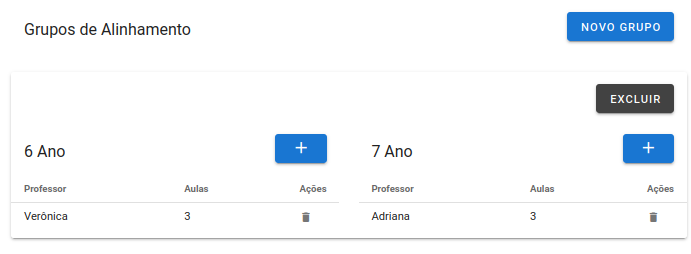
\includegraphics[width=1\textwidth]{./dados/figuras/gruposAlinhamento}
	\fonte{Autor}
	\label{fig:gruposAlinhamento}
\end{figure}
\pagebreak

O efeito da configuração do grupo de alinhamento da figura \ref{fig:gruposAlinhamento}, pode ser observado na grade horária final gerada na figura \ref{fig:alinhados}, com as aulas corretamente alocadas em horários simultâneos.

\begin{figure}[!htb]
	\centering
	\caption{Efeito de grupo de alinhamento}
	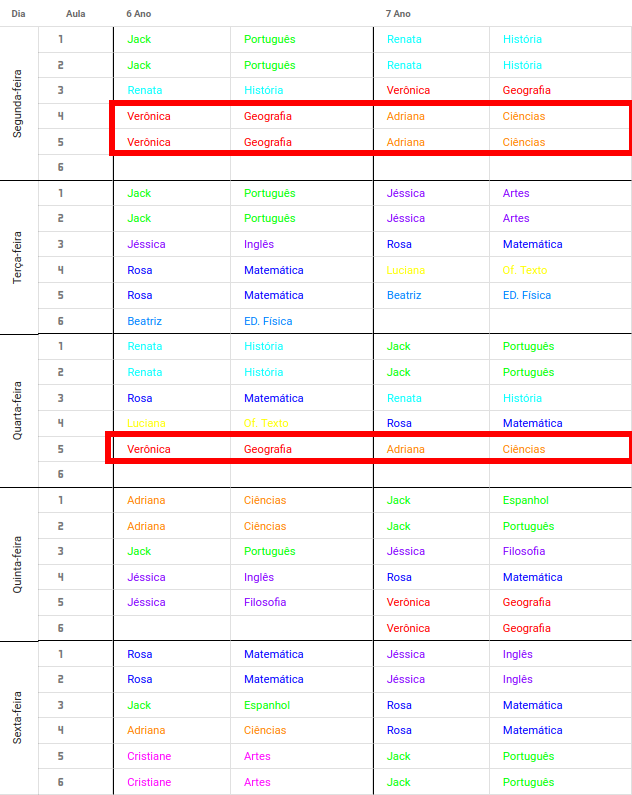
\includegraphics[width=1\textwidth]{./dados/figuras/alinhados}
	\fonte{Autor}
	\label{fig:alinhados}
\end{figure}
\pagebreak

Implementaram-se duas métricas de qualidade relacionadas aos grupos de alinhamento, uma que mensura a quantidade de grupos formados e a quantidade de aulas ``desalinhadas'', ou seja, aulas que deveriam ser agendadas no mesmo horário, mas que não foram.

No caso da \ref{fig:alinhados}, foram formados dois grupos (demarcados em vermelho), e nenhuma aula ficou desalinhada, ou seja, todas as seis aulas configuradas no grupo de alinhamento foram corretamente alocadas em horários simultâneos.

\subsubsection{Janelas}

As janelas consistem em situações em que a jornada de trabalho de determinado professor apresenta um horário sem aulas alocadas, fazendo com que o docente fique ocioso. O quadro \ref{qua:janelas} exemplifica esta situação.

\begin{quadro}[!htb]
	\centering
	\caption{Exemplo de dia com janela.\label{qua:janelas}}
	\begin{tabular}{|p{3cm}|p{3cm}|p{3cm}|p{3cm}|}
		\hline
		\textbf{Aula} & \textbf{6ºAno} & \textbf{7ºAno} & \textbf{8ºAno} \\
		\hline
		1 & Jéssica & Rosa & Adriana \\
		\hline
		2 & Jéssica & Rosa & Adriana \\
		\hline
		3 & Fábio & Jéssica & Rosa \\
		\hline
		4 & Adriana & Jéssica & Rosa \\
		\hline
		5 & Beatriz & Adriana & Jéssica \\
		\hline
	\end{tabular}
	\fonte{Autoria própria}
\end{quadro}

No quadro \ref{qua:janelas}, a professora Adriana tem uma janela na terceira aula, visto que tem aulas alocadas antes e depois (aulas 1, 2, 4 e 5). Em contrapartida, apesar de não ter nenhuma aula planejada no quinto horário, Rosa não tem janelas neste exemplo, pois pode encerrar sua jornada de trabalho na quarta aula.

A métrica de janelas mensura o número de horários na grade que apresentam estes horários ociosos, para cada professor.

\subsubsection{Preferências}

As preferências consistem em configurações que informam ao otimizador características preferíveis para a alocação das aulas de cada professor. Implementaram-se os seguintes tipos de preferência no otimizador:

\begin{enumerate}
	\item Preferência de primeiras aulas;
	\item Preferência de últimas aulas;
	\item Preferência específica de última aula
\end{enumerate}

\begin{figure}[!htb]
	\centering
	\caption{Configuração de preferências}
	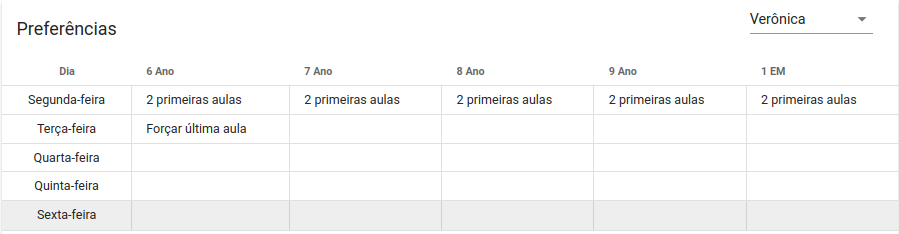
\includegraphics[width=1\textwidth]{./dados/figuras/preferencias}
	\fonte{Autor}
	\label{fig:preferencias}
\end{figure}

A \autoref{fig:preferencias} representa um exemplo de configuração de preferências para determinado professor. Neste caso, a configuração informa ao otimizador que na segunda-feira, as aulas de ``Verônica'' devem ser alocadas desde o início do dia, não ultrapassando um total de aulas; e que na turma do ``6º Ano'', caso haja uma aula dessa professora, esta deve ser alocada na última aula.

Vale ressaltar que o diferencial da preferência específica de última aula é que esta considera a possibilidade de aulas vazias, ou seja, caso o último horário do dia não tenha uma aula alocada, a preferência considera que a aula deve ser alocada na penúltima aula.

\subsubsection{Mínimos e máximos}

Desenvolveram-se métricas de qualidade relacionadas a quantidades de aulas ministradas por dia. Como pode ser visto na figura \ref{fig:tela_minimos}, estas métricas permitem configurar quantidades mínimas e máximas de aulas por dia para cada professor.

\begin{figure}[htb!]
	\centering
	\caption{Mínimos de aulas configuradas na interface}
	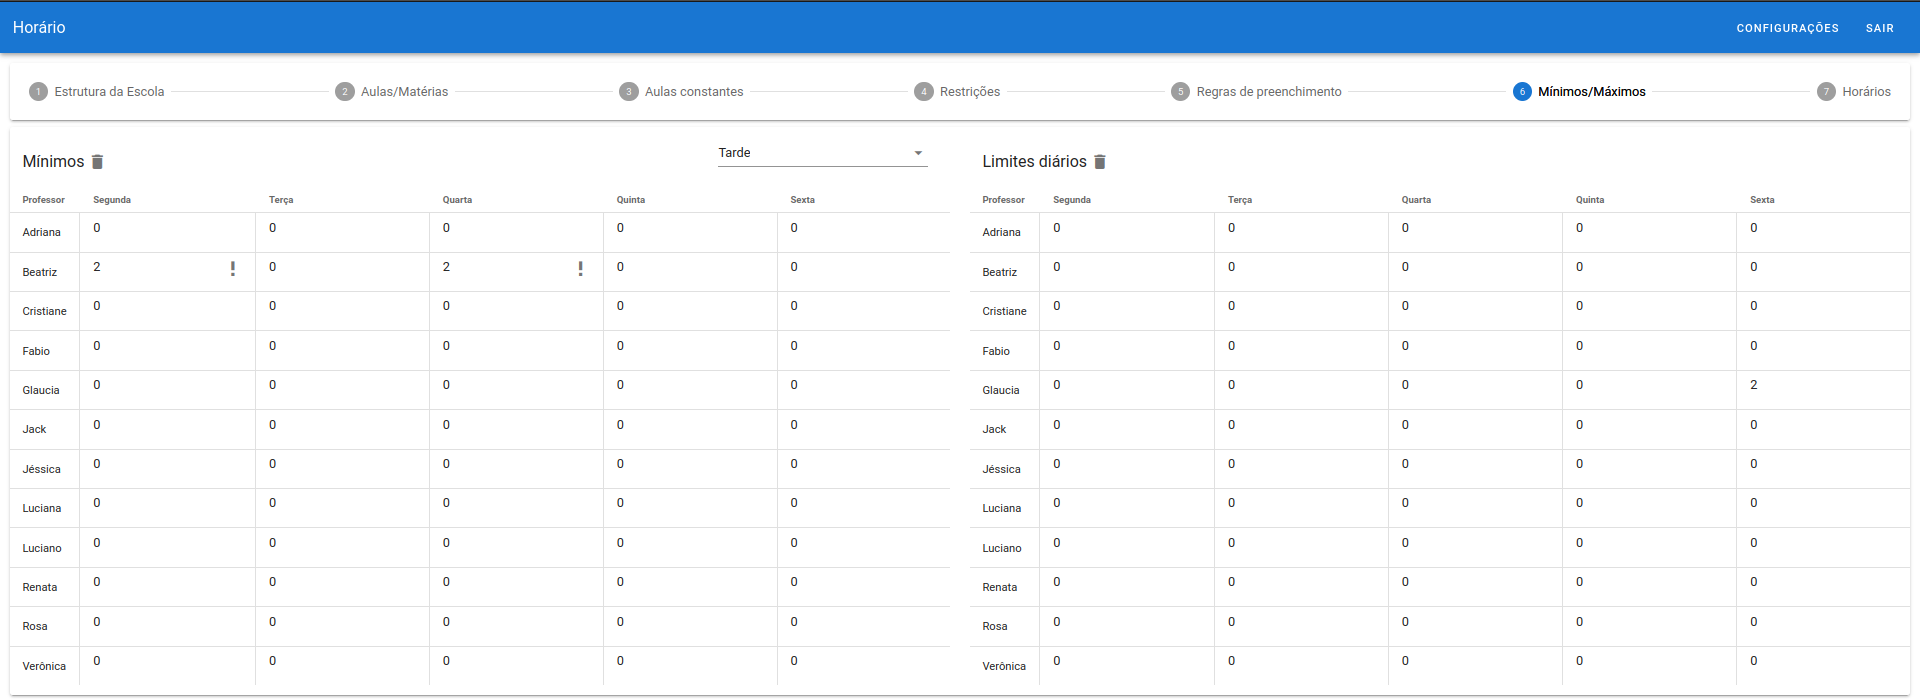
\includegraphics[width=1\textwidth]{./dados/figuras/minimos_configurados}
	\fonte{Autor}
	\label{fig:tela_minimos}
\end{figure}

O cálculo das métricas de qualidade relacionadas aos mínimos e máximos consiste no cálculo do erro, ou seja a quantidade de aulas alocada subtraída da quantidade de aulas esperada. Vale ressaltar que enquanto os mínimos são configuráveis por turno, os máximos são interpretados como limites diários, e consequentemente levam em conta a soma da quantidade de aulas em todos os turnos. Por exemplo, se um professor tem um limite diário de cinco aulas configurado, a soma de suas aulas naquele dia, em todos os turnos, não deverá ultrapassar cinco.

\subsubsection{Armazenamento de soluções}
\label{subsec:salvamento}

Com a adição das métricas, o critério para considerar uma grade horária como uma solução válida ficou mais estrito, e em muitos casos tornou-se impossível obter uma grade que atenda perfeitamente todas as nuances. Tendo isto em mente, foi necessário implementar uma funciondalide de armazenamento de grades horárias um pouco mais detalhada. O resultado disso, pode ser visto no algoritmo \ref{alg:otimizadorComRestricoes}.

\begin{algorithm}
	\caption{Otimizador com persistência de grades horárias}
	\label{alg:otimizadorComRestricoes}
	\KwIn{Lista de professores $LP$, lista de turmas $LT$, matriz de aulas por professor por turma $MA$, temperatura inicial $TI$, Taxa de resfriamento $TR$}
	\KwOut{Grade horária de professores otimizada}
	$temperatura \leftarrow TI$\\
	$grade \leftarrow$ CriaGradeInicial$(LP, LT, MA)$\\
	$iteracoesSemAlteracao \leftarrow 0$\\
	$solucoes \leftarrow$ lista vazia\\
	\While {condição de parada não atingida} {
		$deltaTotal \leftarrow 0$\\
		\For {$passo = 0$ até $numeroPassos$} {
			$turma \leftarrow grade.EscolheTurmaAleatoria()$\\
			$linhas \leftarrow grade.EscolheHorariosAleatoriosValidos(sala)$\\
			$delta \leftarrow grade.CalculaDelta(sala, linhas)$\\
			$probabilidade \leftarrow e^{-delta/temperatura}$\\
			$valorAceite \leftarrow Aleatorio(0, 1)$\\
			\If {$delta < 0$ ou $probabilidade \ge valorAceite$} {
				$grade.PermutaProfessores(sala, linha1, linha2)$\\
				$deltaTotal \leftarrow deltaTotal + delta$\\
				\If {grade não existe na lista de soluções} {
					insere grade na lista de soluções\\
					limita lista de soluções às 100 melhores grades\\
				}
			}
		}
		\eIf {$delta = 0$} {
			$iteracoesSemAlteracao \leftarrow iteracoesSemAlteracao + 1$\\
		}{
			$iteracoesSemAlteracao \leftarrow 0$\\
		}
		\If {$iteracoesSemAlteracao \ge 15$} {
			salvaGradesRelevantes()\\
			apaga lista de soluções\\
			$temperatura \leftarrow TI$\\
			$iteracoesSemAlteracao \leftarrow 0$\\
		}
		$temperatura \leftarrow temperatura * TR$
	}
\end{algorithm}
\pagebreak

Consinderando as diversas métricas de qualidade que as grades horárias passaram a ter, o método ``salvaGradesRelevantes'' do algoritmo \ref{alg:otimizadorComRestricoes} salva, para cada métrica escolhida, as 5 grades que tiveram a melhor pontuação em cada métrica. A princípio, optou-se por utilizar as métricas de qualidade geral (média ponderada de todas as métricas), janelas, agrupamento de aulas e número de preferências resolvidas, mas este método pode ser expandido para qualquer uma das métricas implementadas no sistema.


\section{SERVIDOR E BANCO DE DADOS}

A aplicação do lado do servidor é responsável por receber as requisições da interface, persistir as configurações no banco de dados e realizar a comunicação com o otimizador, a fim de produzir e armazenar as grades horárias.

Para o desenvolvimento deste componente, optou-se pelo \textit{framework Express.js}, a ser executado na plataforma \textit{Node.js}, devido à simplicidade de implementação que estas tecnologias proporcionam. Em relação ao banco de dados, será utilizado o sistema de gerenciamento de banco de dados \textit{PostgresSQL}, devido à sua robustez.

Conforme as premissas do problema sendo tratado, a modelagem do banco de dados é centrada na entidade ``Configuração'', que agrupa as configurações de determinada instituição de ensino para a geração de suas grades horárias. Cada uma dessas entidades tem turnos, salas, professores, e as configurações de quantas aulas cada professor deve ministrar em cada sala, e as respectivas restrições.

A modelagem comentada está representada na \autoref{fig:diagramaEr}:

\begin{figure}[!htb]
	\centering
	\caption{Modelo Entidade-Relacionamento}
	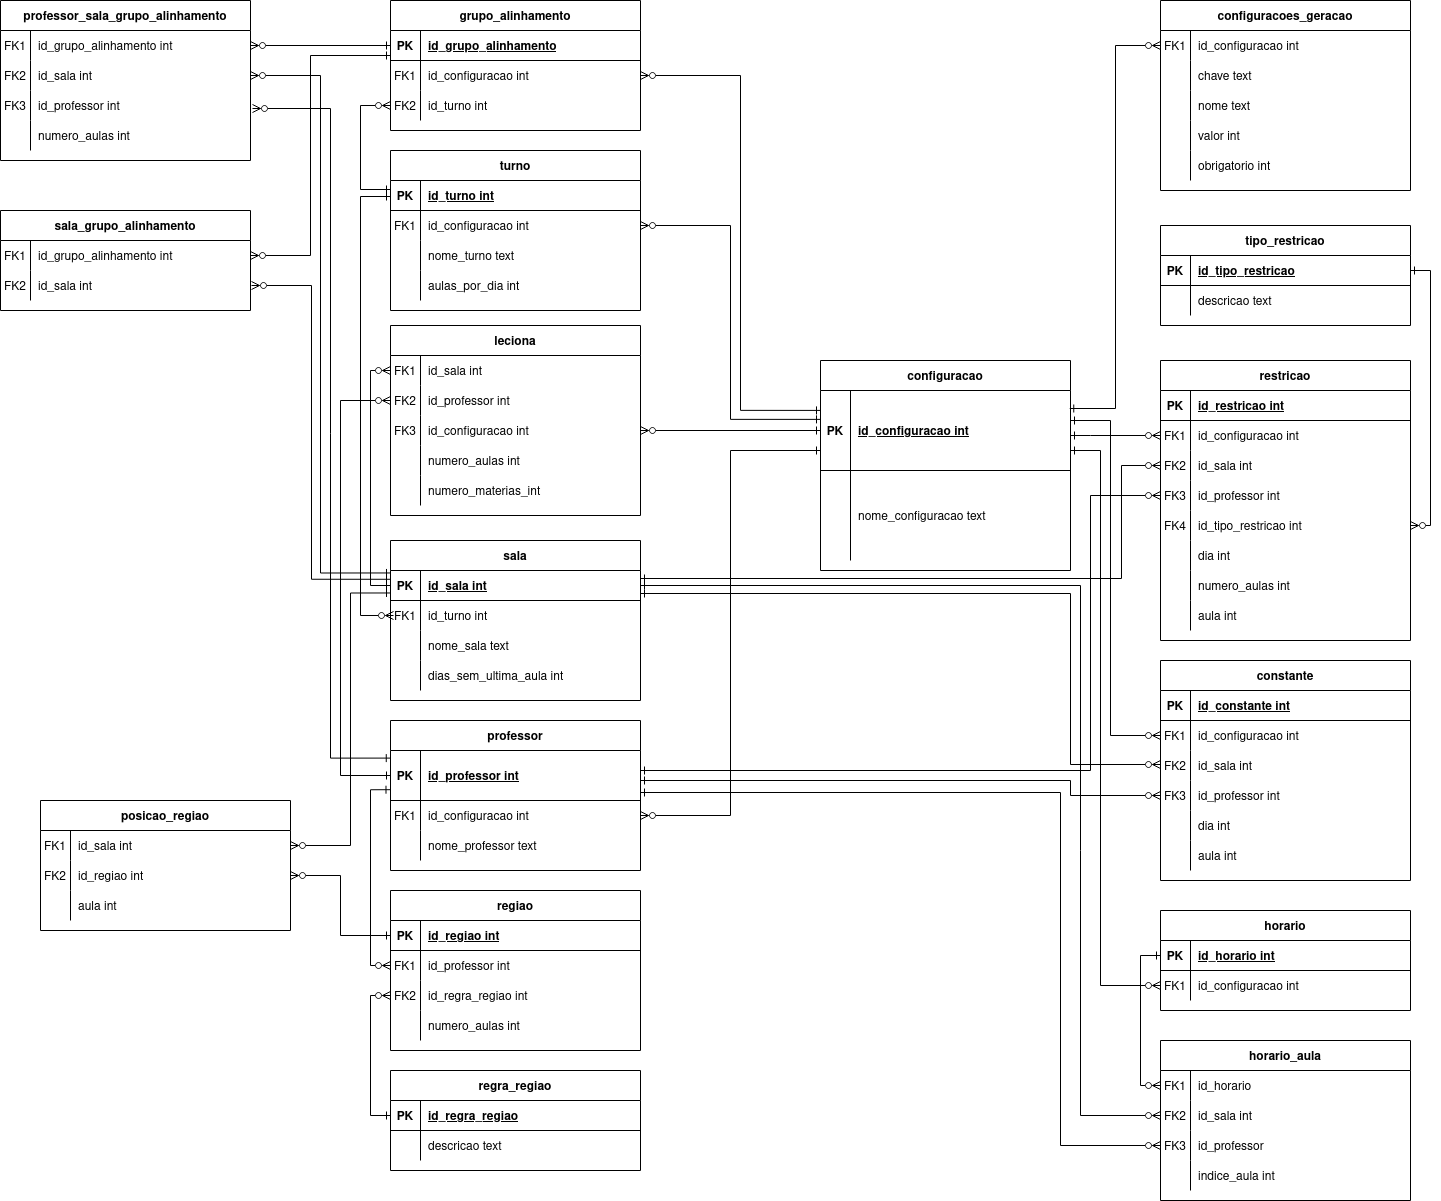
\includegraphics[width=1\textwidth]{./dados/figuras/diagrama_er}
	\fonte{Autor}
	\label{fig:diagramaEr}
\end{figure}
\newpage

Dentre as entidades mostradas no modelo entidade-relacionamento, vale ressaltar a importância da entidade ``Grupo Alinhamento''. Esta será utilizada para configurar aulas que devam acontecer simultaneamente, a fim de resolver o desafio dos itinerários formativos do Novo Ensino Médio, conforme exposto na seção \ref{sec:novo_ensino_medio}.

Para validar a modelagem do banco de dados, realizaram-se inserções de informações de exemplo nas diferentes tabelas. A \autoref{fig:sqlValidacao} mostra algumas dessas inserções e os vínculos instituídos pelos identificadores escolhidos.

\begin{figure}[!htb]
	\centering
	\caption{Consultas de validação da modelagem}
	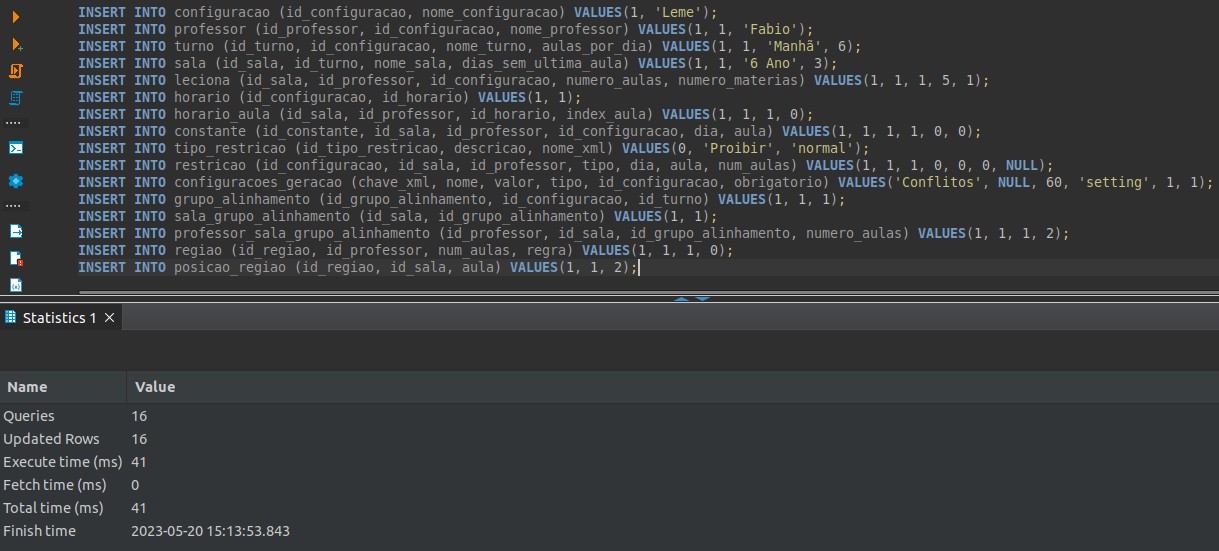
\includegraphics[width=1\textwidth]{./dados/figuras/sql_validacao}
	\fonte{Autor}
	\label{fig:sqlValidacao}
\end{figure}
\newpage

Validou-se também o armazenamento das grades horárias no banco de dados. A \autoref{fig:sqlGrade} traz um exemplo de consulta de uma grade horária com sete salas:

\begin{figure}[!htb]
	\centering
	\caption{Consulta SQL de grade horária com sete salas}
	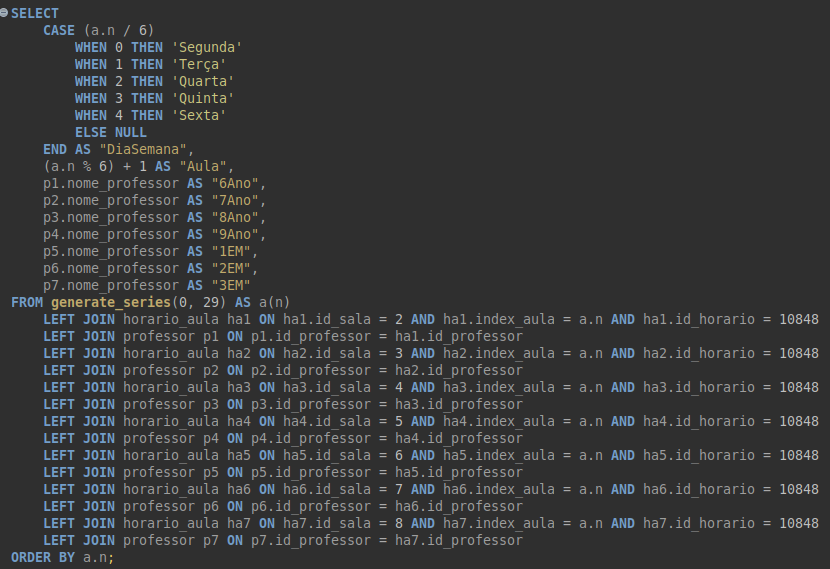
\includegraphics[width=0.7\textwidth]{./dados/figuras/sql_grade}
	\fonte{Autor}
	\label{fig:sqlGrade}
\end{figure}

A consulta anterior traz como resultado a tabela visível na \autoref{fig:consultaGrade}, com linhas e colunas correpondentes a horários de aulas e salas respectivamente.

\begin{figure}[!htb]
	\centering
	\caption{Resultado da consulta de uma grade no banco de dados}
	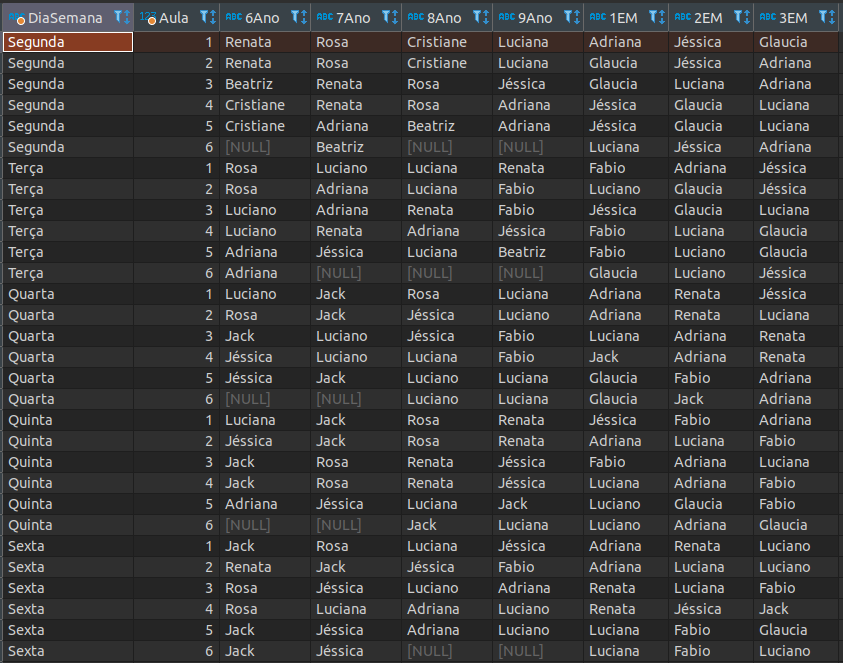
\includegraphics[width=0.7\textwidth]{./dados/figuras/ConsultaGrade}
	\fonte{Autor}
	\label{fig:consultaGrade}
\end{figure}
\section{INTERFACE}

A interface \textit{web} será responsável pela interação do usuário final com a aplicação. Portanto, deverá implementar funcionalidades que possibilitem a configuração das restrições e características das grades horárias a serem geradas, além de mostrar ou exportar tais grades após a geração.

Para o desenvolvimento deste componente, optou-se pelo framework \textit{Vue.js}, devido à riqueza de seu ecossistema de desenvolvimento \textit{frontend} e familiaridade do graduando com este. Complementando este framework, será utilizado também o \textit{Vuetify.js}, a fim de facilitar e padronizar o design da aplicação.

A \autoref{fig:diagrama-uc} mostra os casos de uso que a interface \textit{web} será responsável por disponibilizar:

\begin{figure}[!htb]
	\centering
	\caption{Diagrama de Casos de Uso}
	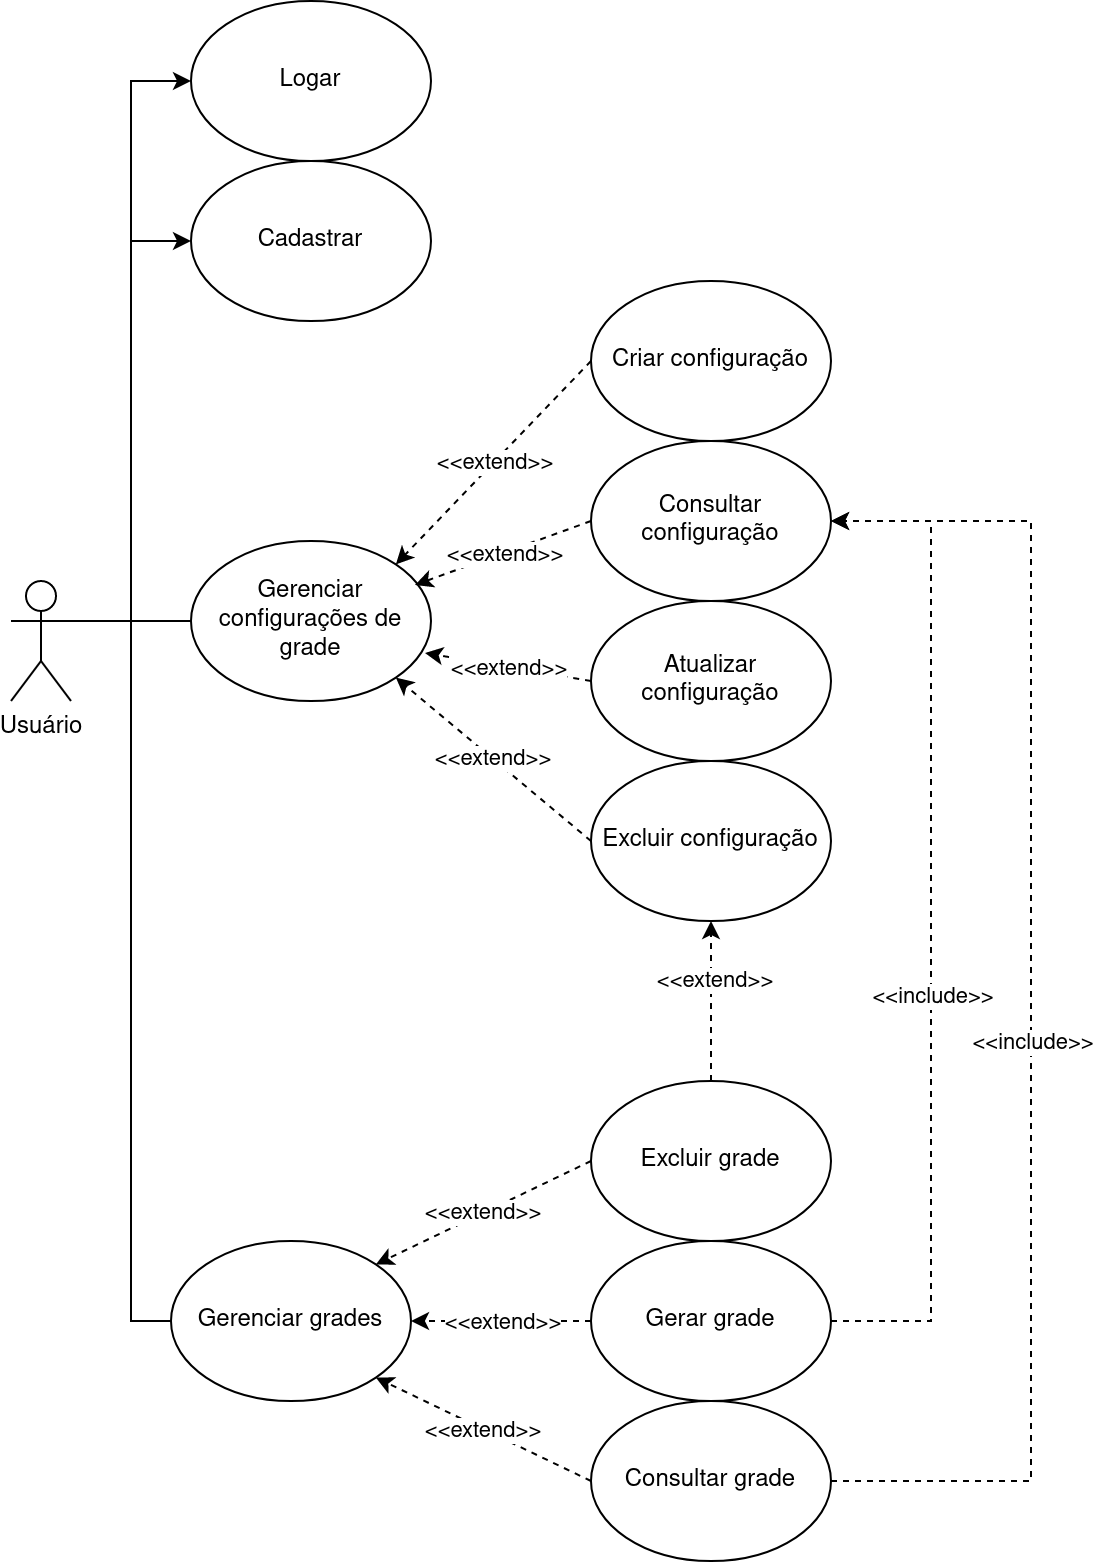
\includegraphics[width=0.65\textwidth]{./dados/figuras/diagrama_uc}
	\fonte{Autor}
	\label{fig:diagrama-uc}
\end{figure}
\newpage

Desenvolveram-se alguns protótipos iniciais das telas necessárias na aplicação.
Primeiramente, a \autoref{fig:tela-configuracoes} mostra a tela de listagem de configurações de grade. Como comentado anteriormente, alguns dos casos de uso da aplicação envolvem o gerenciamento de configurações de grades horárias, as quais são listadas nessa tela.

\begin{figure}[!htb]
	\centering
	\caption{Tela - Listagem de Configurações de Grade}
	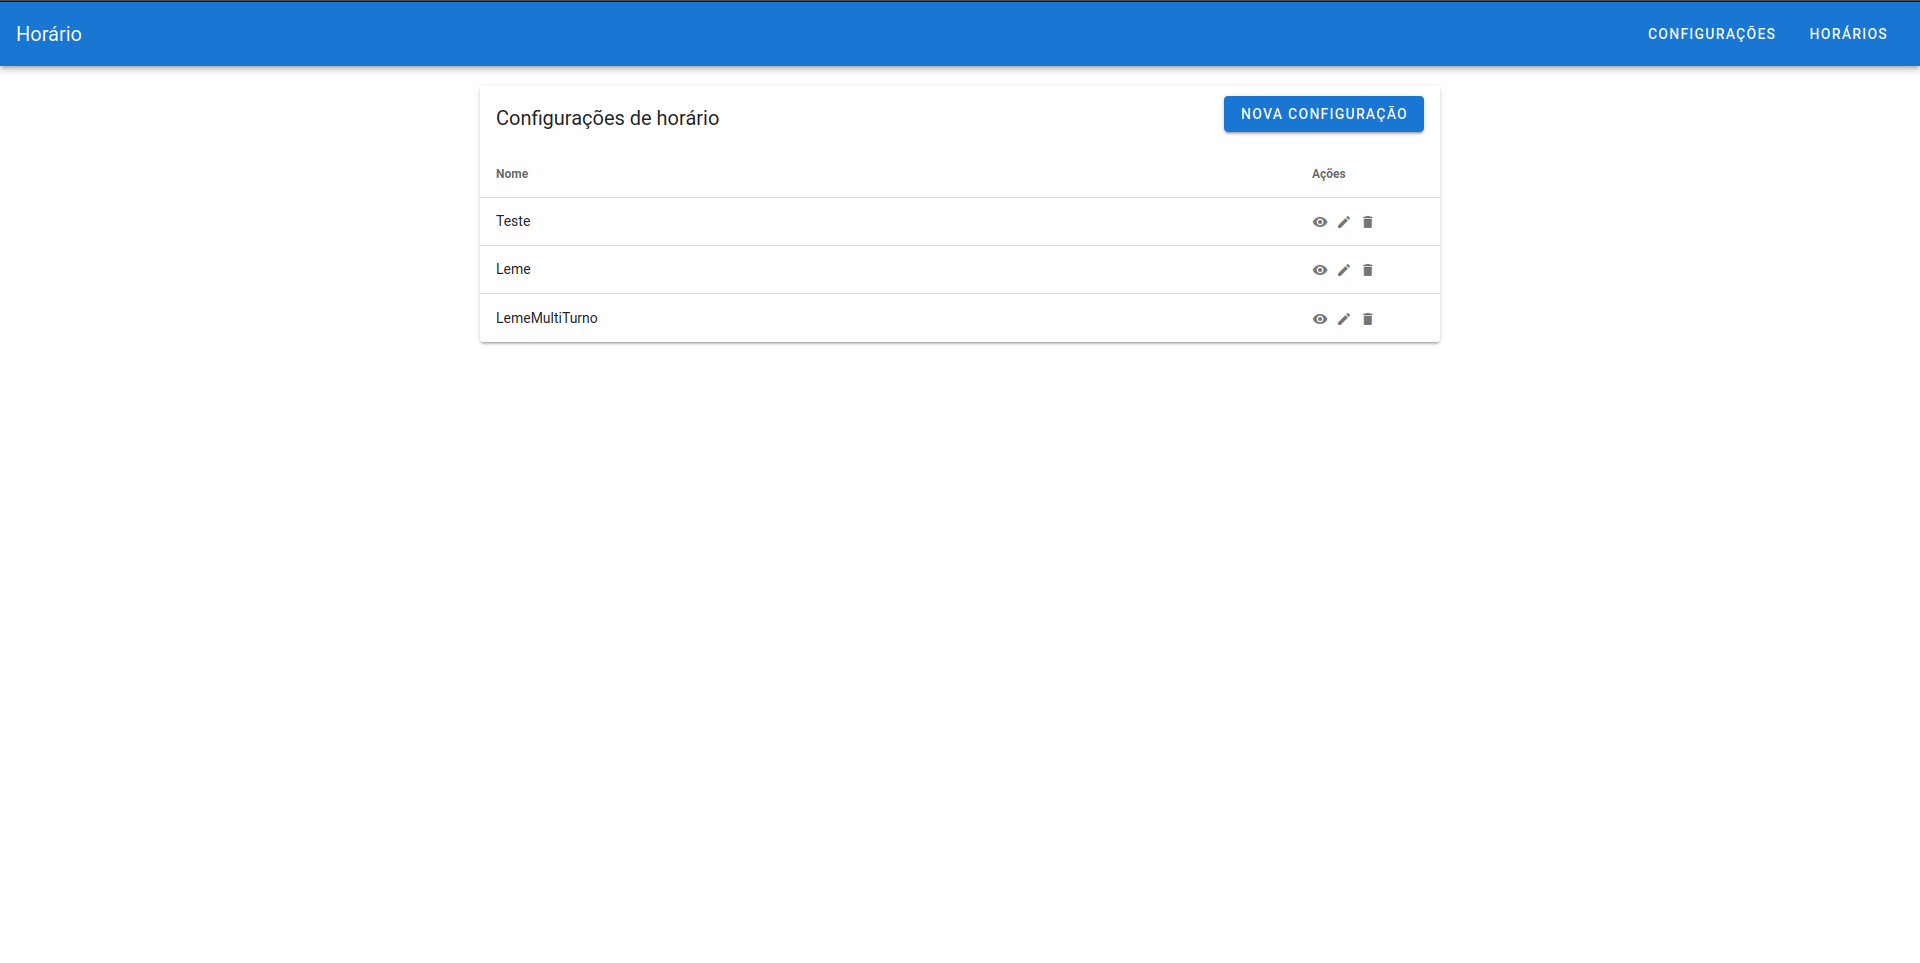
\includegraphics[width=0.8\textwidth]{./dados/figuras/tela_configuracoes}
	\fonte{Autor}
	\label{fig:tela-configuracoes}
\end{figure}
\pagebreak

A tela mostrada na \autoref{fig:tela-estrutura1} é responsável por permitir que o usuário cadastre os professores da escola. Nessa tela é possível notar que a aplicação foi estruturada seguindo uma noção de etapas de configuração até a geração da grade horária final. No topo da tela, a etapa "Estrutura da Escola" encontra-se selecionada.

\begin{figure}[!htb]
	\centering
	\caption{Tela - Estrutura da Escola - Professores}
	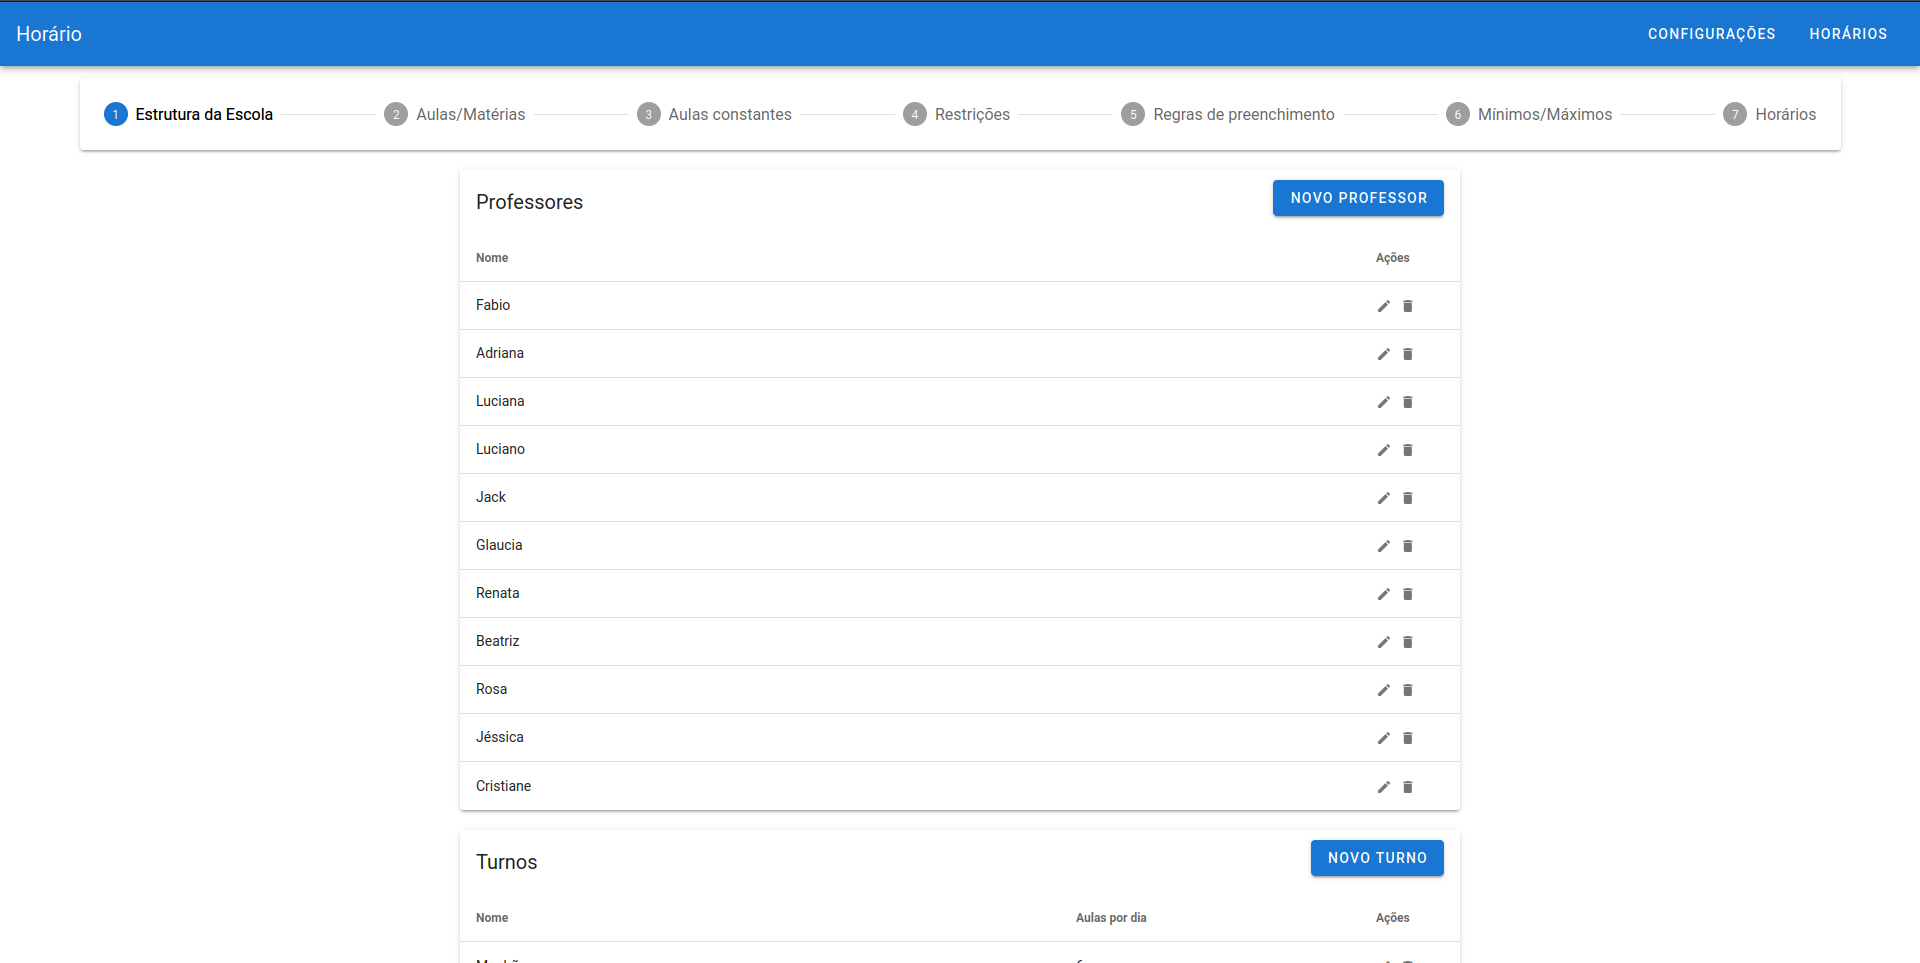
\includegraphics[width=0.8\textwidth]{./dados/figuras/tela_estrutura1}
	\fonte{Autor}
	\label{fig:tela-estrutura1}
\end{figure}
\newpage

Na \autoref{fig:tela-estrutura2}, tem-se a continuação da tela de estrutura da escola, mostrada na \autoref{fig:tela-estrutura1}. Esta parte da tela é responsável pela configuração das salas e turnos da escola.

\begin{figure}[!htb]
	\centering
	\caption{Tela - Estrutura da Escola - Salas e Turnos}
	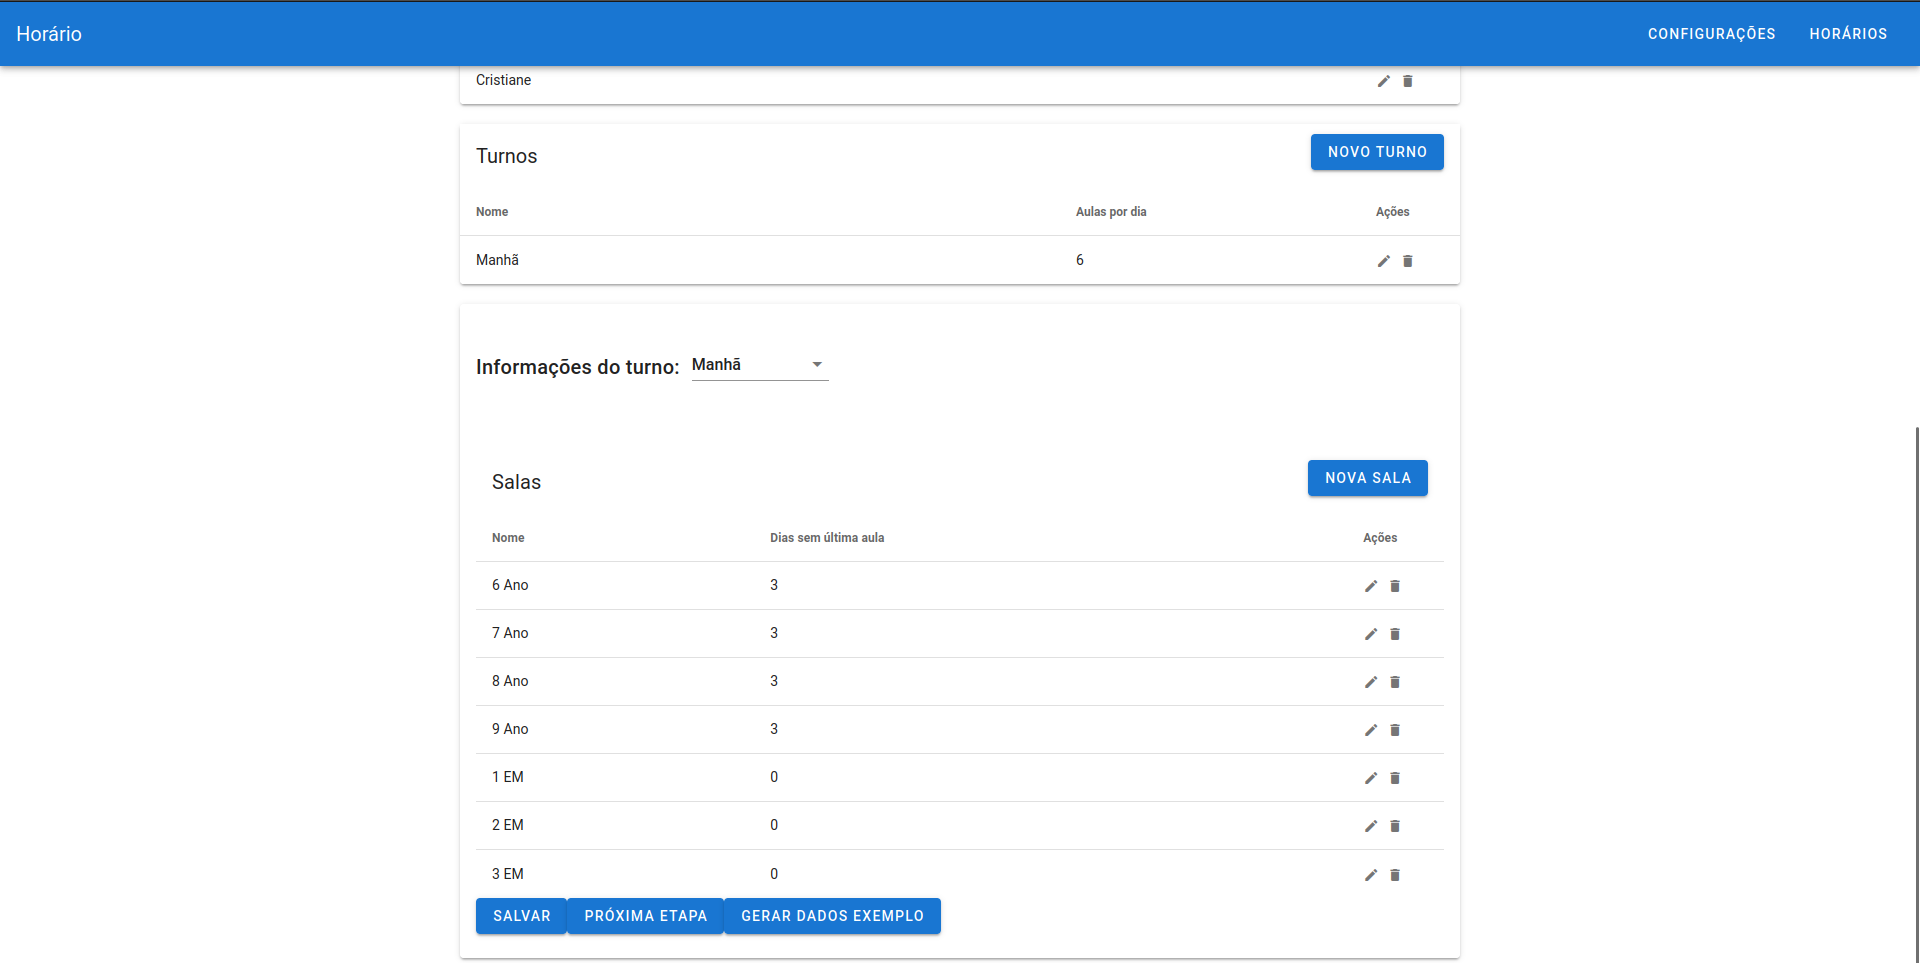
\includegraphics[width=0.8\textwidth]{./dados/figuras/tela_estrutura2}
	\fonte{Autor}
	\label{fig:tela-estrutura2}
\end{figure}

Na tela da \autoref{fig:tela-aulas}, o usuário pode realizar a configuração de número de aulas que cada professor deve ministrar em cada sala, informação fundamental para a geração das grades horárias.

\begin{figure}[!htb]
	\centering
	\caption{Tela - Aulas por professor}
	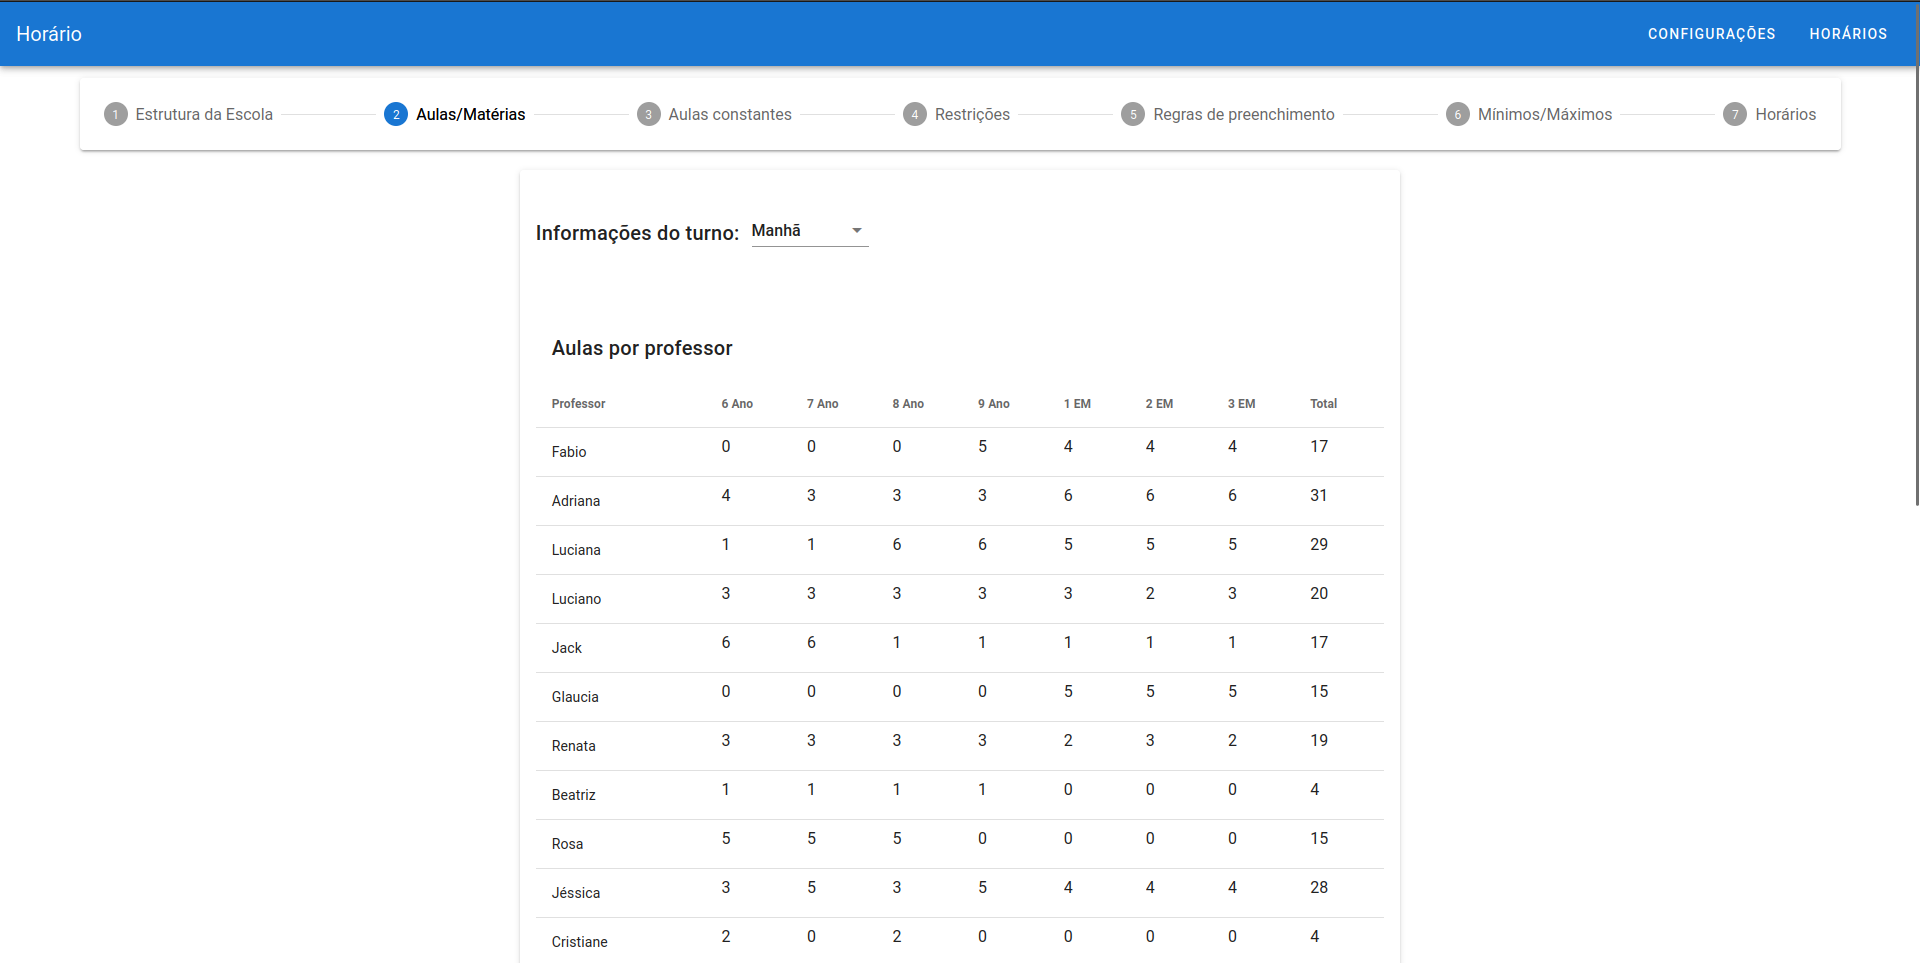
\includegraphics[width=0.8\textwidth]{./dados/figuras/tela_aulas}
	\fonte{Autor}
	\label{fig:tela-aulas}
\end{figure}
\newpage

A tela da \autoref{fig:tela-restricoes} é responsável pela configuração das restrições. Nesta, o usuário pode configurar horários na grade que devem ser evitados ou proibidos para determinado docente.

\begin{figure}[!htb]
	\centering
	\caption{Tela - Restrições}
	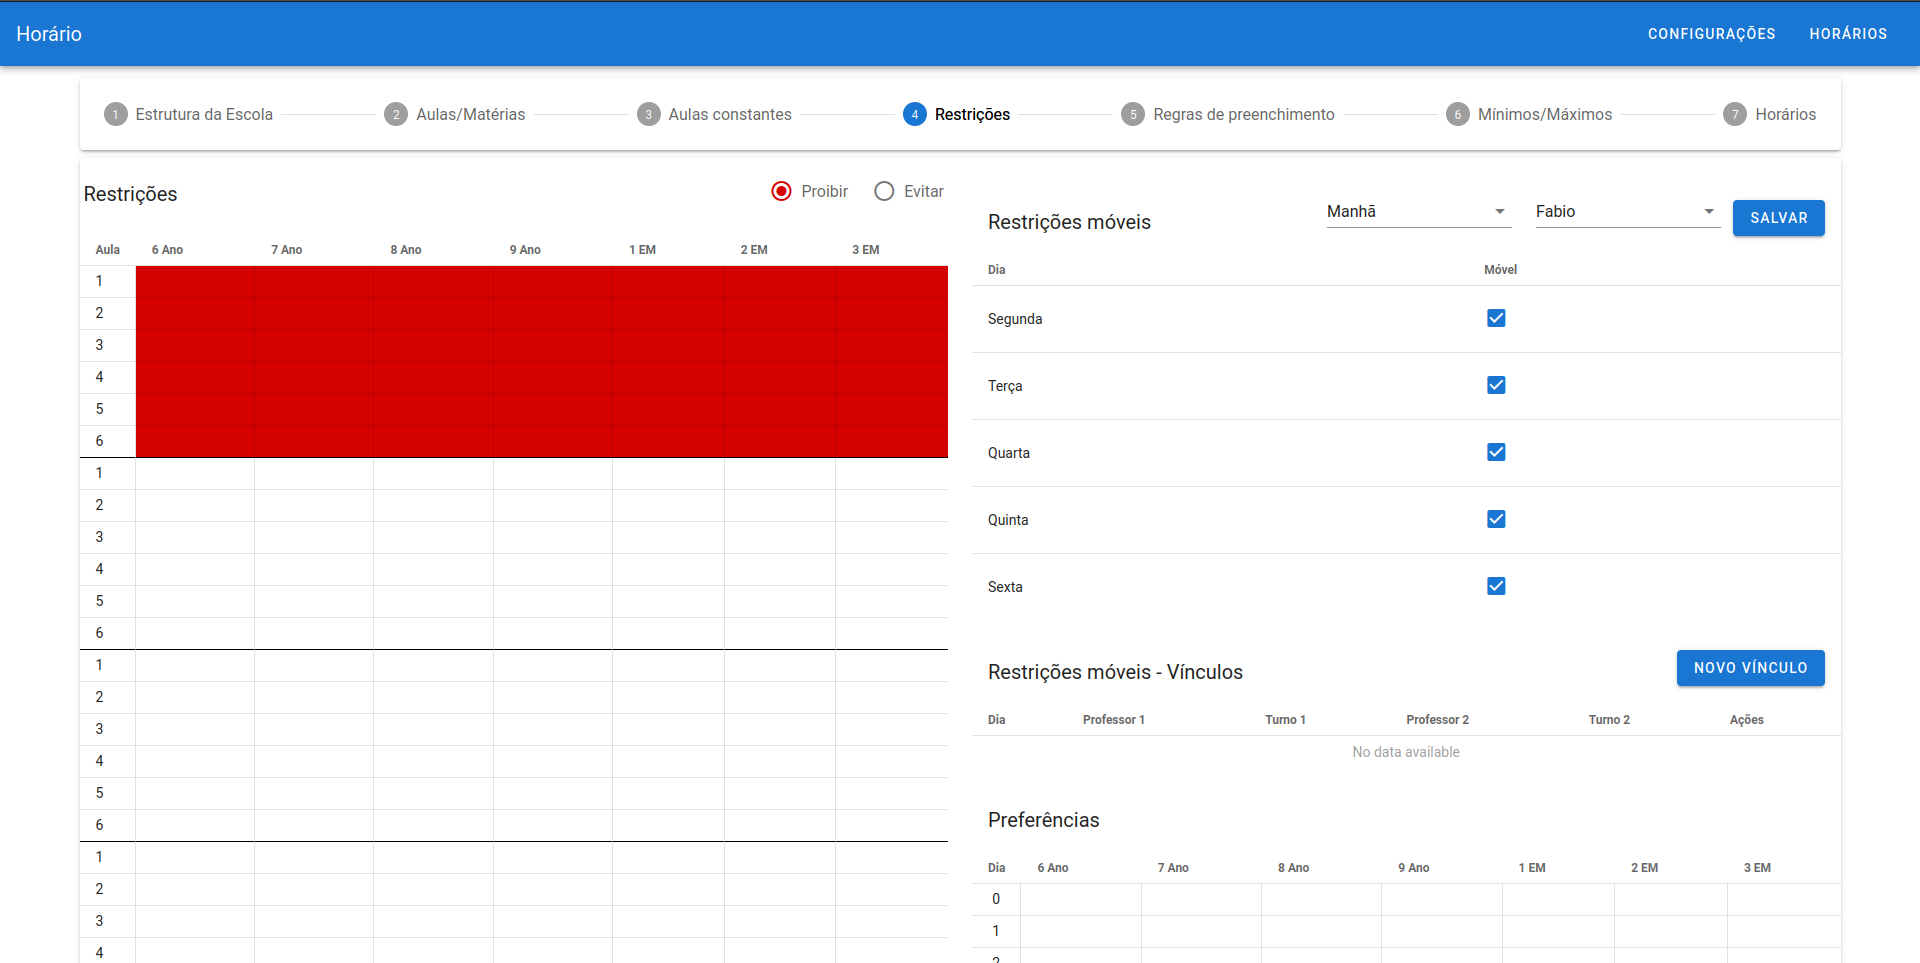
\includegraphics[width=0.8\textwidth]{./dados/figuras/tela_restricoes}
	\fonte{Autor}
	\label{fig:tela-restricoes}
\end{figure}

A última etapa no fluxo da aplicação é representada pela tela da \autoref{fig:tela-horarios}. Nesta, o usuário pode requisitar a geração da grade horária utilizando as configurações realizadas nas etapas anteriores, e acessar as grades geradas anteriormente.

\begin{figure}[!htb]
	\centering
	\caption{Tela - Horários}
	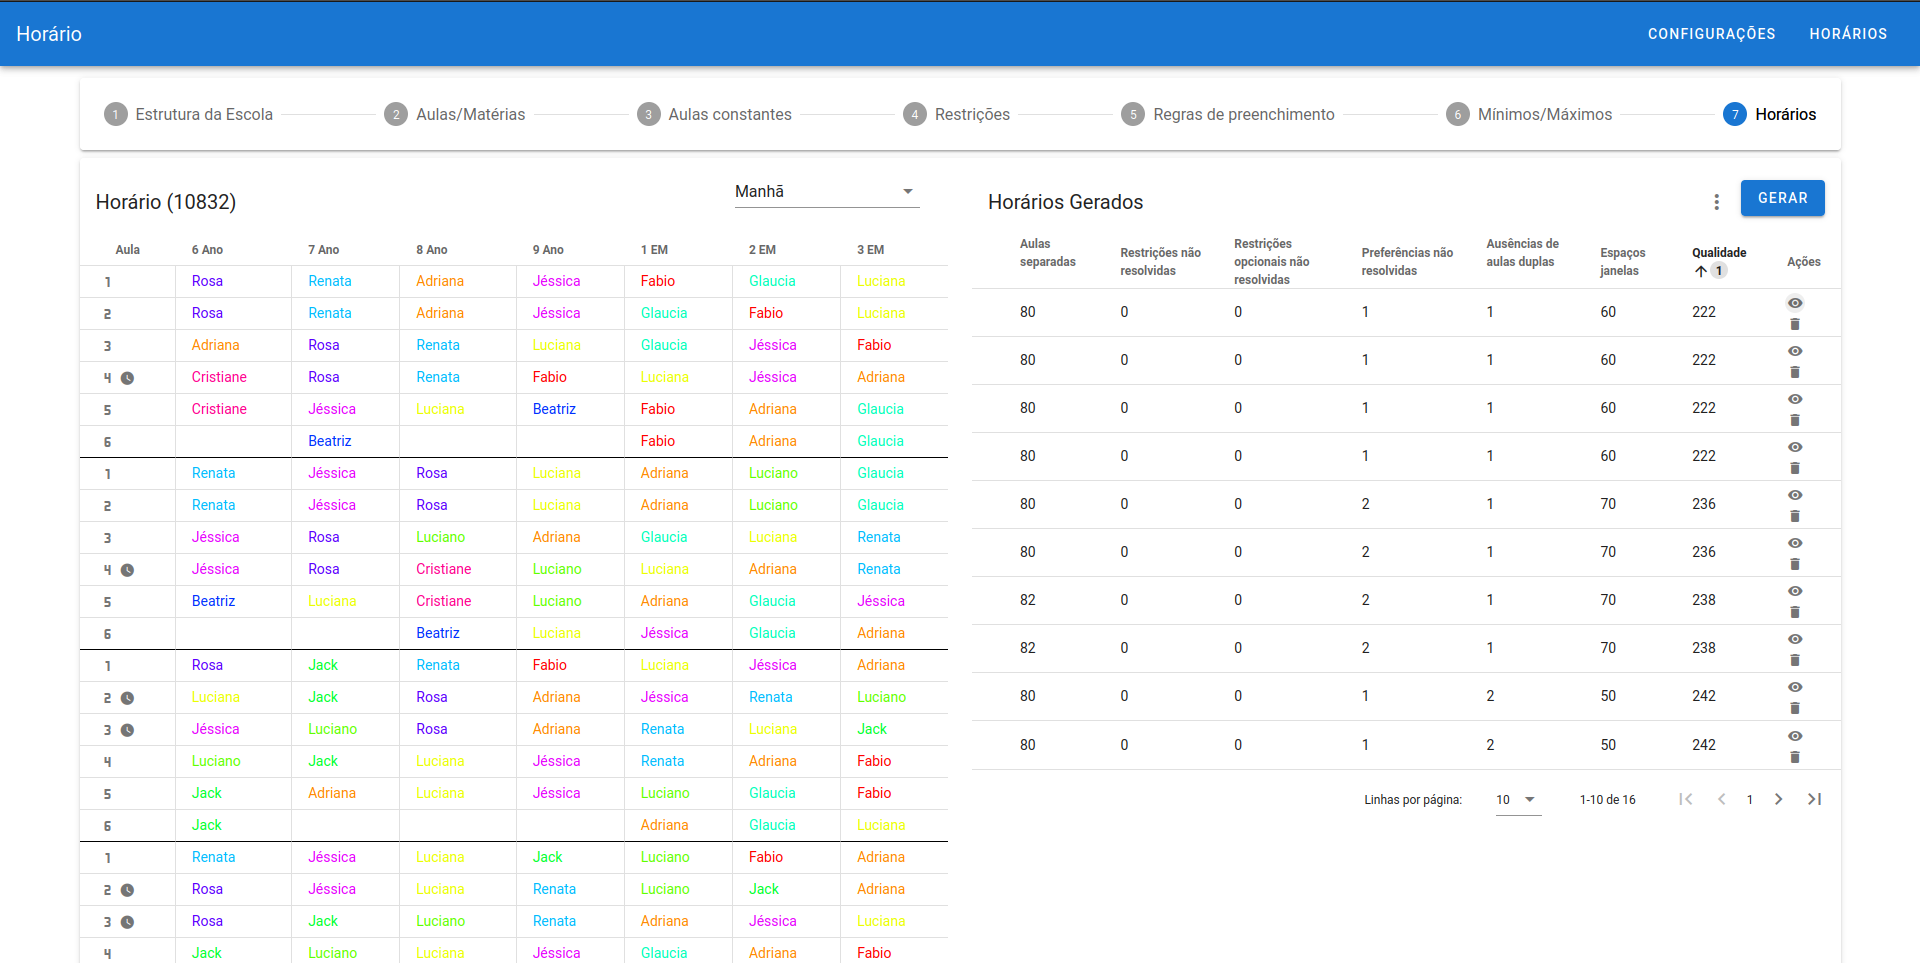
\includegraphics[width=0.8\textwidth]{./dados/figuras/tela_horarios}
	\fonte{Autor}
	\label{fig:tela-horarios}
\end{figure}
\newpage
\subsection{USUÁRIOS E AUTENTICAÇÃO}

Para controlar a visibilidade de informações no sistema desenvolvido, implementou-se um sistema de usuários. A melhoria consistiu na:

\begin{enumerate}
	\item Criação de tabela de usuários no banco de dados;
	\item Associação da tabela ``configuracao'' com a tabela de usuários, para que fosse possível armazenar o usuário responsável por cada configuração;
	\item Criação da tela de login na interface web;
	\item Criação das rotas de cadastro e \textit{login} no servidor
	\item Criação do \textit{middleware} de autenticação
	\item Criação do \textit{middleware} de validação da configuração
\end{enumerate}

\subsubsection{Adaptação do banco de dados}
A aplicação dos itens 1 e 2 foi realizada diretamente no banco de dados, através da criação da tabela mencionada e a chave estrangeira possibilitando a associação de cada usuário a múltiplas configurações. Após estas alterações, o diagrama entidade relacionamento do banco de dados passa a ser representado pela figura \ref{fig:er_atualizado}.

\begin{figure}[!htb]
	\centering
	\caption{Modelo Entidade-Relacionamento com adição da tabela de usuários}
	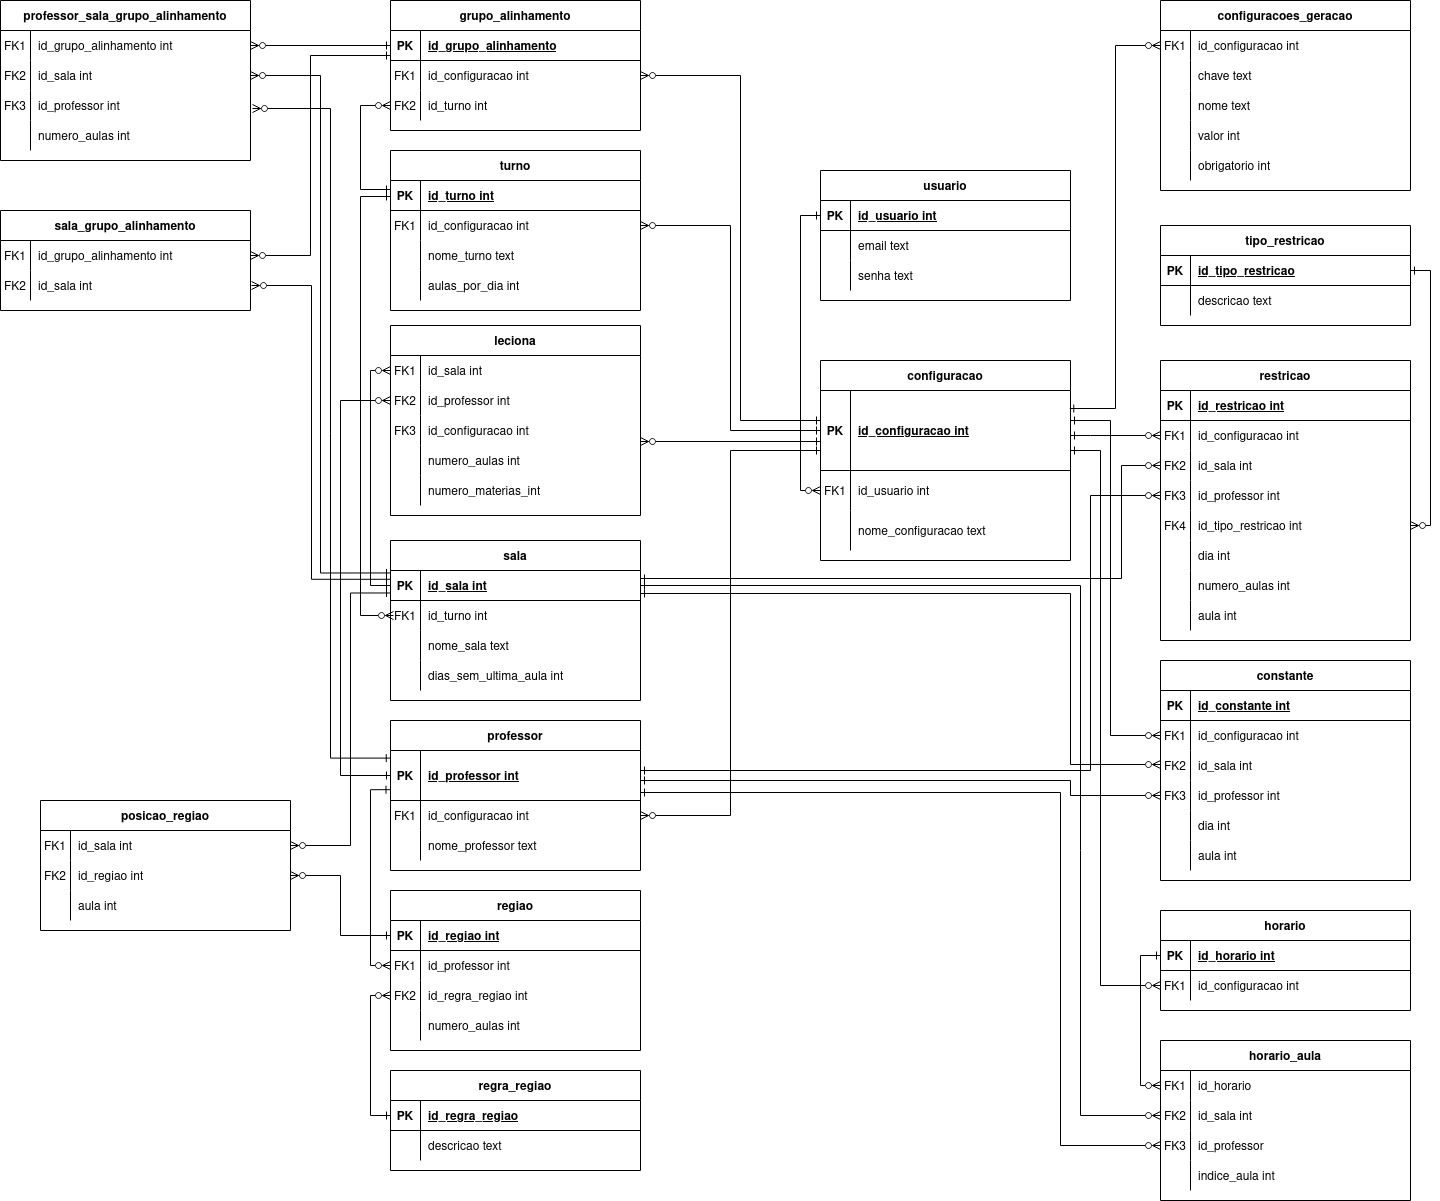
\includegraphics[width=0.65\textwidth]{./dados/figuras/er_horario_com_usuario}
	\fonte{Autor}
	\label{fig:er_atualizado}
\end{figure}

\subsubsection{Tela de login}
Como pode ser visto na figura \ref{fig:login}, desenvolveu-se uma tela simples de \textit{login}, a qual também desempenha a função de cadastro de novos usuários.

\begin{figure}[!htb]
	\centering
	\caption{Tela de Acesso}
	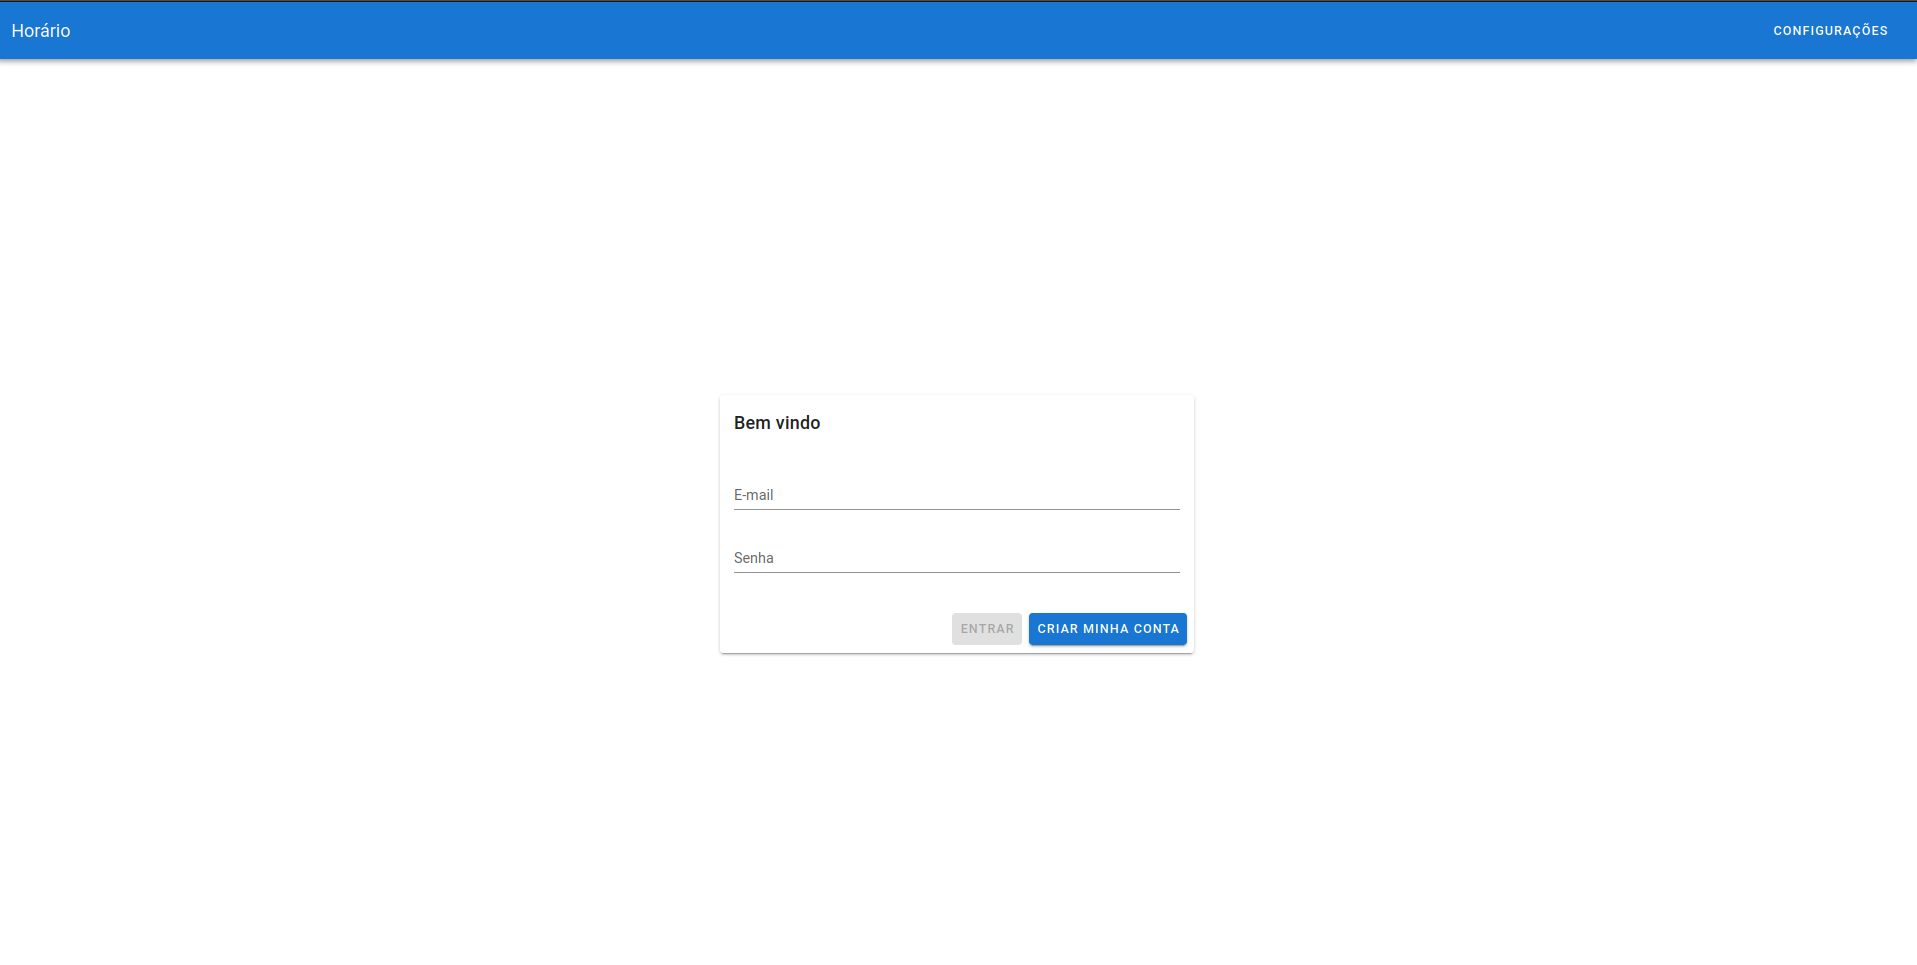
\includegraphics[width=1\textwidth]{./dados/figuras/telaLogin}
	\fonte{Autor}
	\label{fig:login}
\end{figure}
\pagebreak

\subsubsection{Rotas de autenticação}
Para a implementação das rotas de cadastro e \textit{login}, utilizou-se além do \textit{framework ExpressJS}, os pacotes JWT (\textit{Json Web Token}) e \textit{bcrypt}. O pacote JWT é utilizado para gerar \textit{tokens}, que são enviados para a interface web e podem ser utilizados para autenticar os usuários; já o \textit{bcrypt} é utilizado para gerar e validars as \textit{hashes} das senhas dos usuários, para que nunca sejam armazenadas senhas em texto pleno no banco de dados.

A função utilizada pela nova rota de cadastro pode vista na figura \ref{fig:metodoCadastro}. A função ``register'' realiza a validação dos parâmetros, e cria um usuário no banco de dados, caso já não exista outro com o mesmo e-mail. Além disso, a função retorna um \textit{token} JWT para a interface web, para que seja possível verificar a autenticidade das próximas requisições realizadas pelo usuário. 

\begin{figure}[!htb]
	\centering
	\caption{Método de Cadastro}
	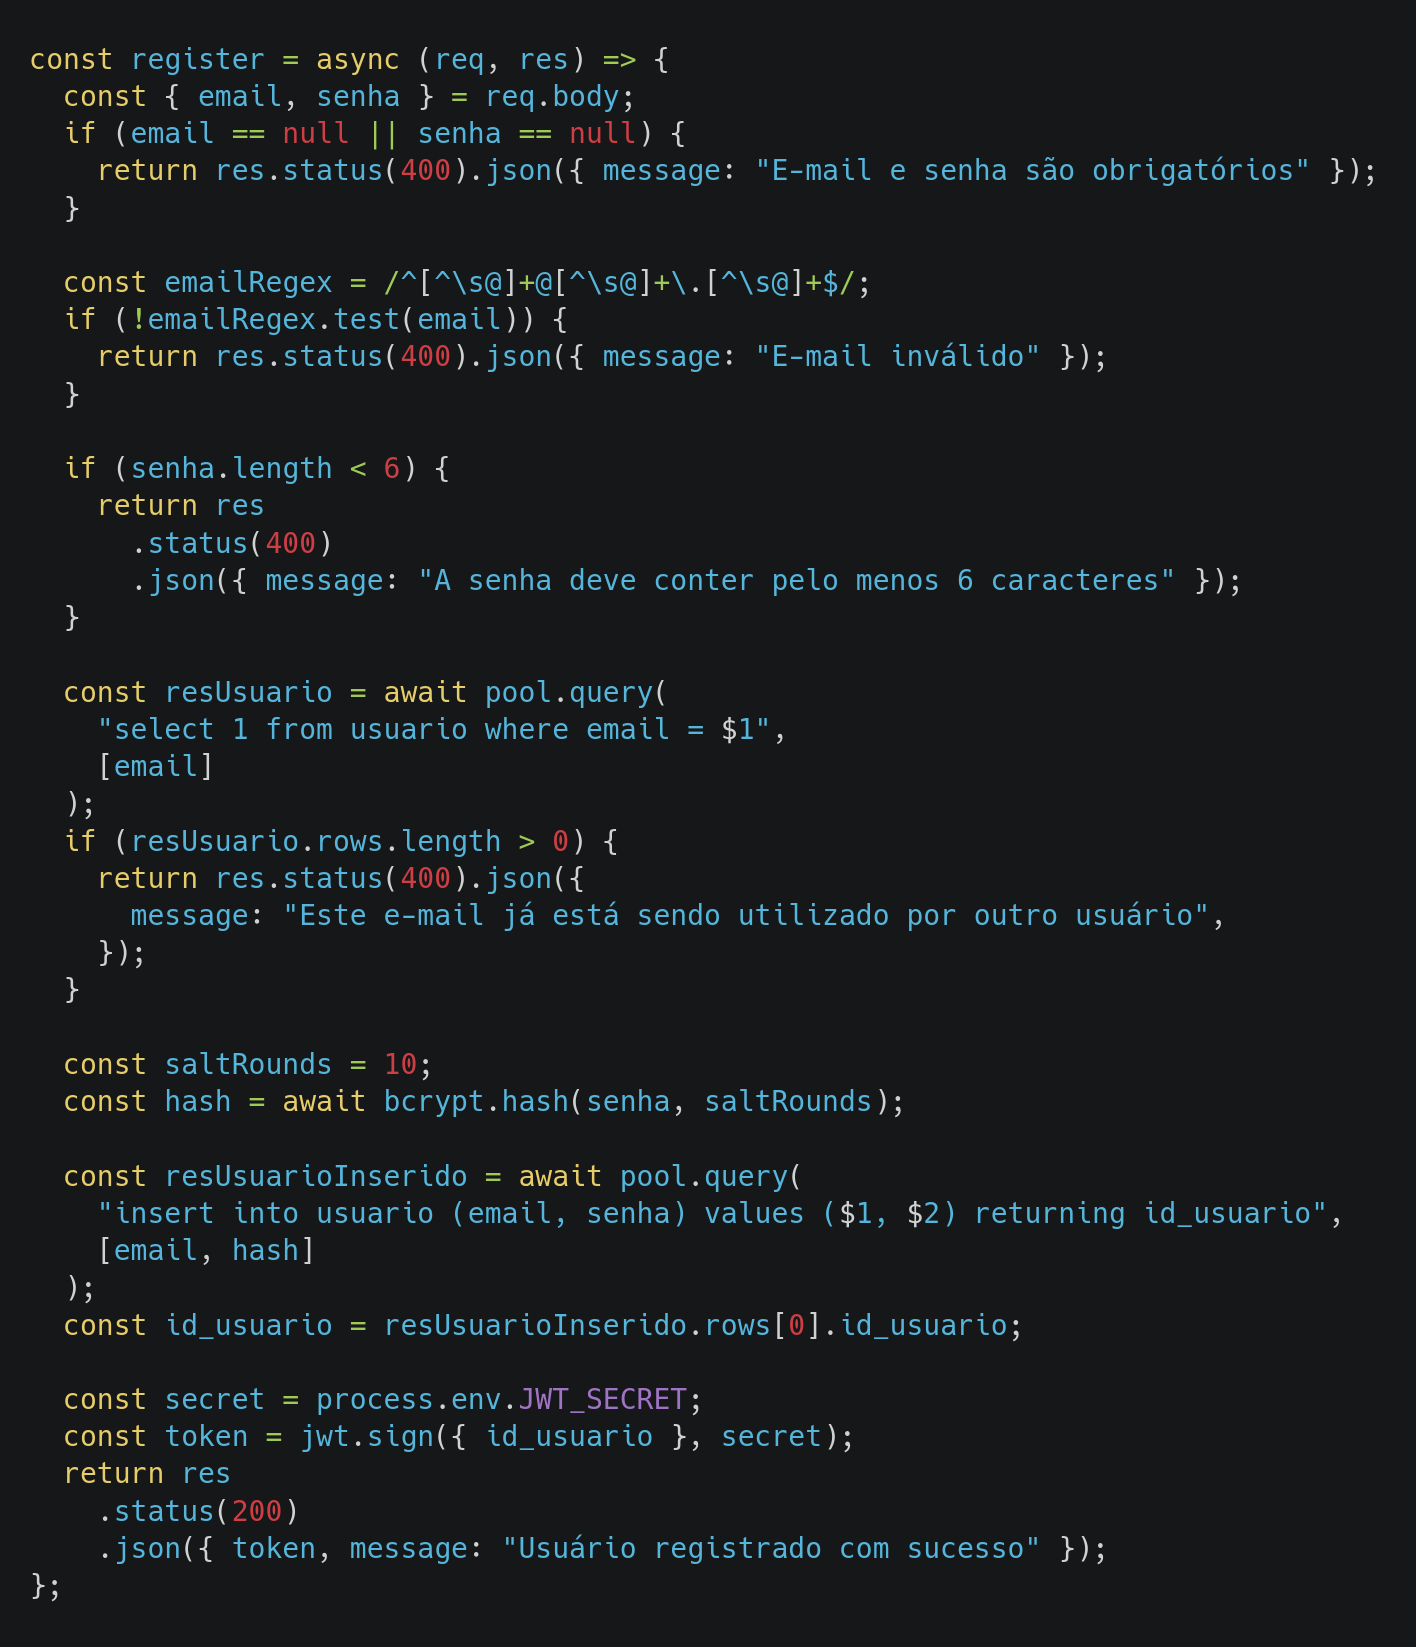
\includegraphics[width=0.8\textwidth]{./dados/figuras/register}
	\fonte{Autor}
	\label{fig:metodoCadastro}
\end{figure}
\pagebreak

A função de \textit{login}, visível na figura \ref{fig:metodoLogin} é similar, realizando validação dos parâmetros, autenticação do usuário através da comparação de senhas utilizando o pacote \textit{bcrypt} e geração de \textit{token} JWT. Vale citar que em ambas as rotas de autenticação, é inserido no \textit{payload} do \textit{token} o identificador do usuário, que posteriormente pode ser utilizado pelos \textit{middlewares} para a realização de validações.

\begin{figure}[!htb]
	\centering
	\caption{Método de Login}
	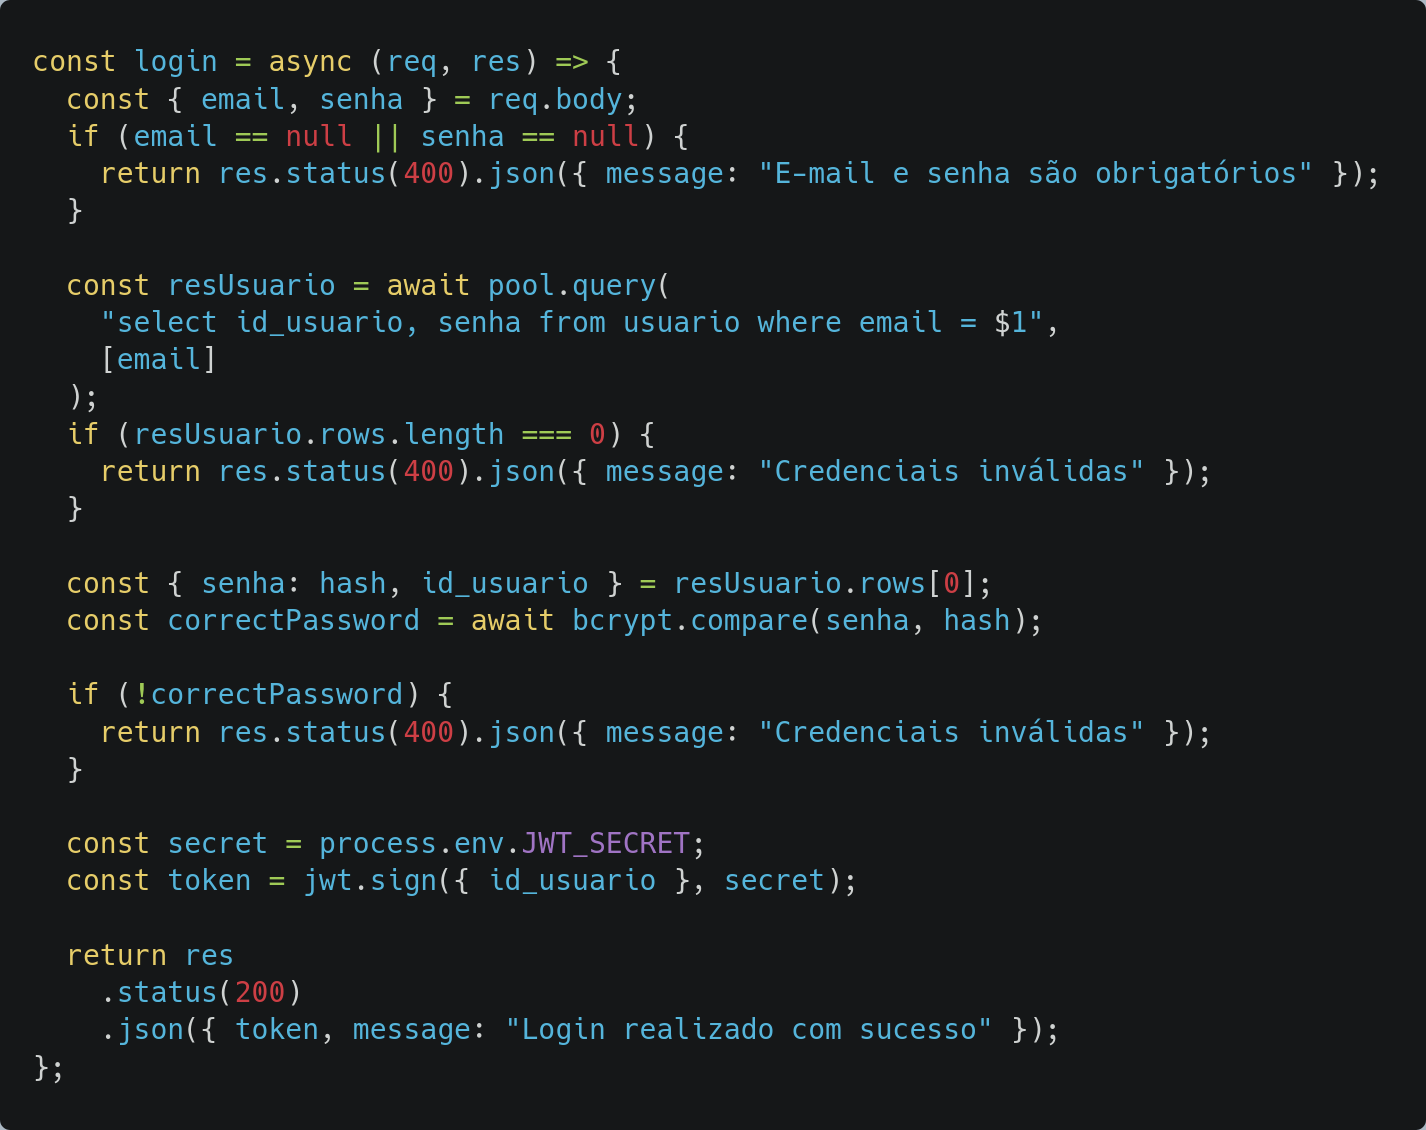
\includegraphics[width=0.8\textwidth]{./dados/figuras/login}
	\fonte{Autor}
	\label{fig:metodoLogin}
\end{figure}
\pagebreak

\subsubsection{Middlewares}
Foram criadas duas funções \textit{middleware} relacionadas aos usuários. A primeira é responsável por assegurar que apenas usuários propriamente autenticados tenham acesso aos recursos protegidos do sistema. Como pode ser visto na figura \ref{fig:auth}, essa verificação é realizada através da verificação da presença de um \textit{token} JWT válido no \textit{header ``authorization''} da requisição.

\begin{figure}[!htb]
	\centering
	\caption{Middleware de autenticação}
	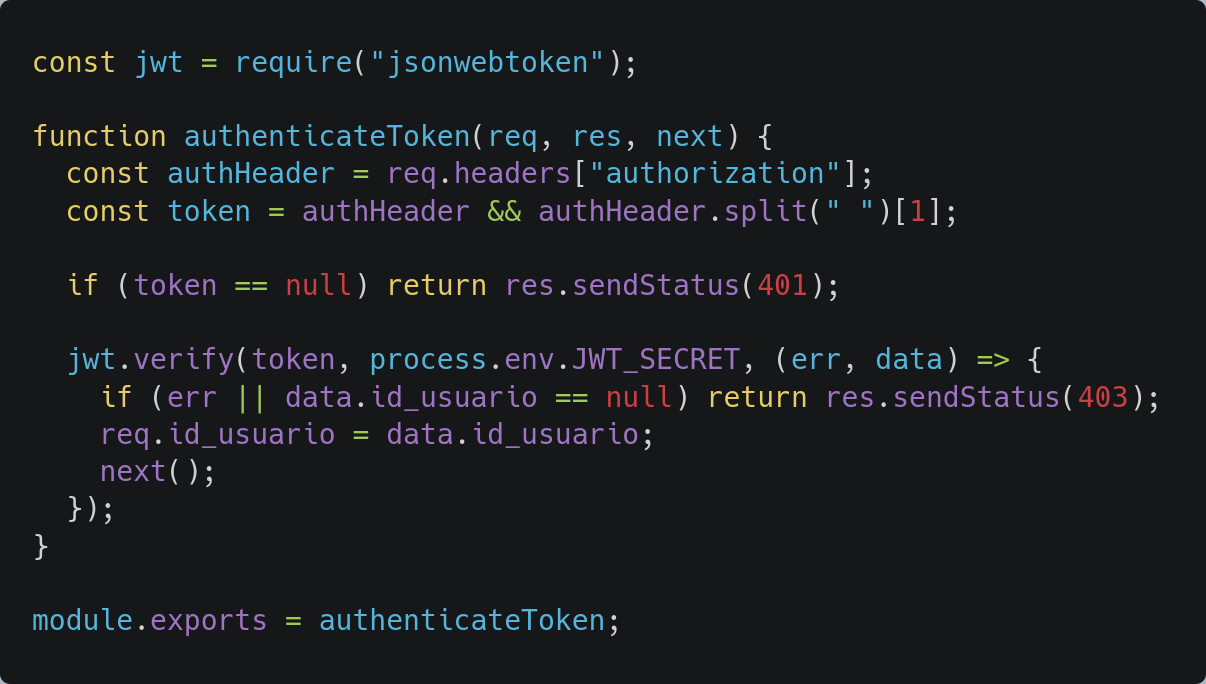
\includegraphics[width=0.8\textwidth]{./dados/figuras/authMiddleware}
	\fonte{Autor}
	\label{fig:auth}
\end{figure}
\pagebreak

O outro middleware criado tem como objetivo assegurar que um usuário possa consultar apenas as configurações pelas quais seja responsável. Isso é feito utilizando o identificador do usuário, presente no \textit{payload} do \textit{token} JWT, conforme a figura \ref{fig:configMiddleware}. Caso o usuário não tenha um vínculo com a configuração que está tentando acessar, a requisição é bloqueada.

\begin{figure}[!htb]
	\centering
	\caption{Middleware de validação da configuração}
	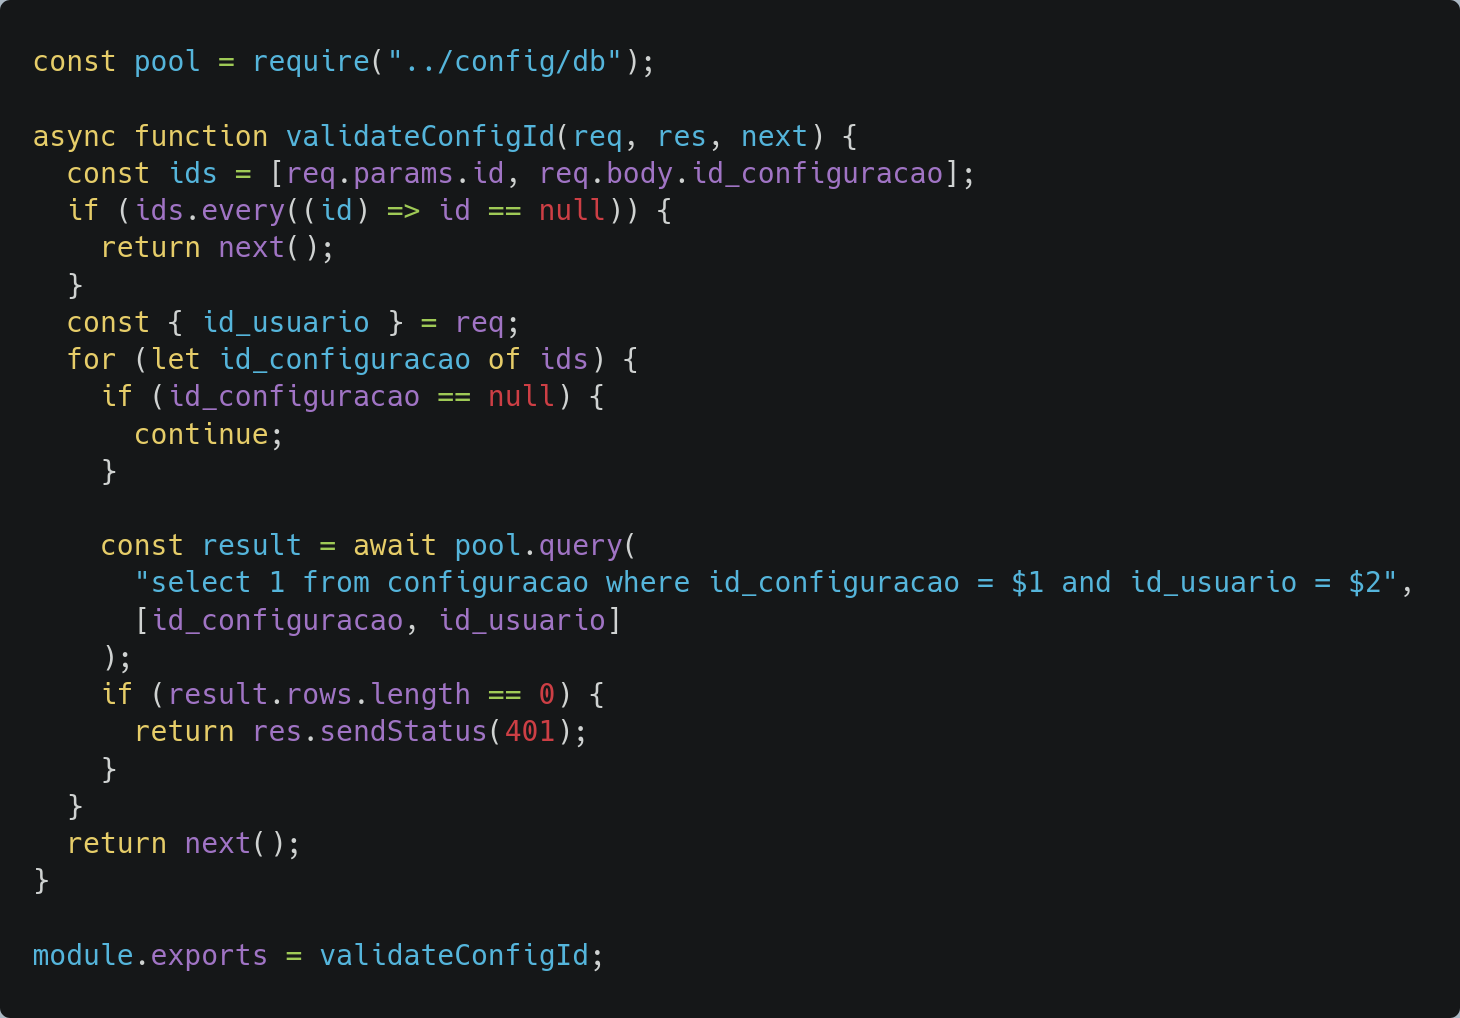
\includegraphics[width=0.8\textwidth]{./dados/figuras/configMiddleware}
	\fonte{Autor}
	\label{fig:configMiddleware}
\end{figure}
\pagebreak



\subsection{ALOCAÇÃO DE MATÉRIAS}

Durante os incrementos anterioriores, o otimizador gerava grades horárias que continham apenas os nomes dos professores alocados para aula. Em outras palavras, as grades eram matrizes nas quais as linhas eram os horários disponíveis, as colunas eram as salas e cada posição na matriz representava qual professor deveria ministrar a aula naquele horário.

A alocação dos professores é muito importante para a resolução do problema, pois apresenta a maior parte das retrições e dificuldades relacionadas, como os conflitos, por exemplo. Entretando, em termos de completude, as grades horárias devem ter também a alocação de matérias em cada horário de aula, visto que cada professor pode ministrar aulas de mais de uma matéria. As alterações necessárias para possibilitar isso foram:

\begin{enumerate}
	\item Alterar a modelagem do banco de dados para comportar informações relacionadas às matérias;
	\item Alterar telas da interface web para que fosse possível configurar as matérias;
	\item Alterar rotas do servidor para persistir as matérias;
	\item Alterar código do otimizador para produzir grades horárias com matérias
\end{enumerate}

\subsubsection{Alteração no banco de dados}
Para armazenar informações relacionadas às matérias, a modelagem do banco de dados foi alterada com a criação de três tabelas: 
\begin{itemize}
	\item materia
	\item horario-materias: representa uma grade horária de matérias, que tem vínculo com a entidade principal da grade horária
	\item horario-materia: representa uma matéria alocada em determinada posição de uma grade horária
\end{itemize}

Com esta modelagem atualizada, presente na figura \ref{fig:modelagemMateiras}, cada grade horária de professores, pode ter diferentes opções de grades de matérias.

\begin{figure}[!htb]
	\centering
	\caption{Modelo Entidade-Relacionamento com Matérias}
	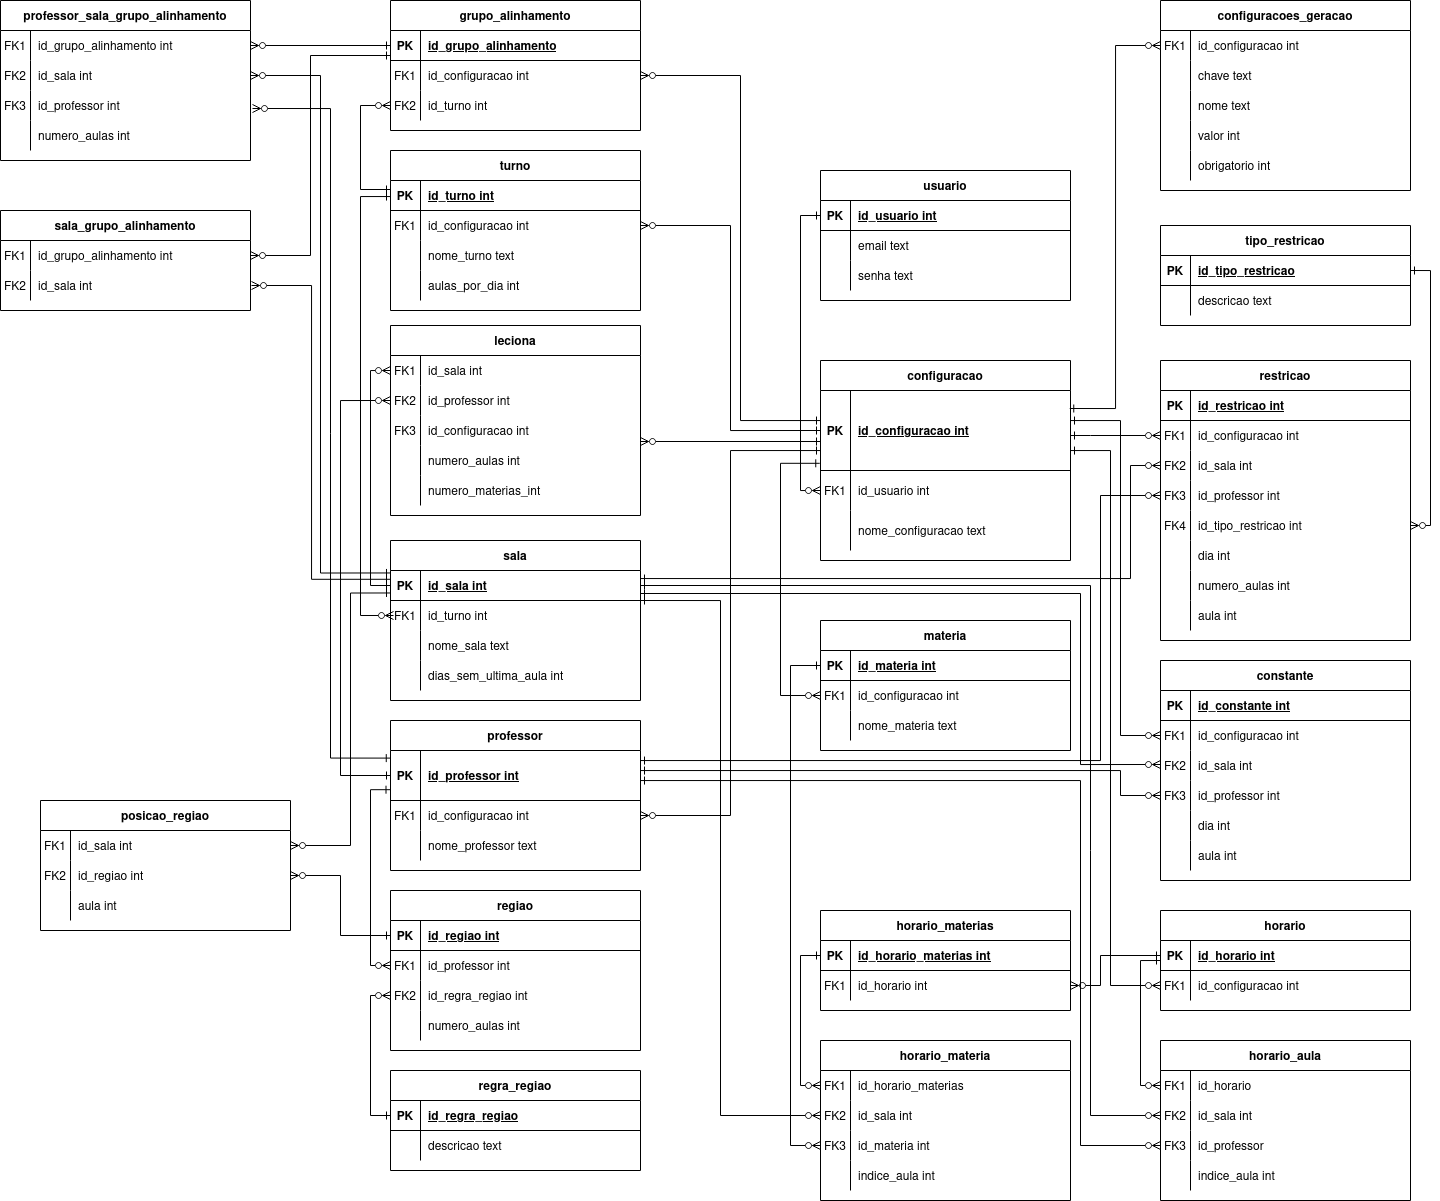
\includegraphics[width=0.65\textwidth]{./dados/figuras/er_materias}
	\fonte{Autor}
	\label{fig:modelagemMateiras}
\end{figure}
\pagebreak

\subsubsection{Alteração de telas}
Com a adição do conceito das matérias ao sistema, algumas telas da interface precisaram ser modificadas. A primeira destas, foi a tela inicial da configuração, ou seja, a tela de "Estrutura da Escola", cuja alteração pode ser vista na figura \ref{fig:estruturaAtualizada} consistiu na adição de uma seção para cadastro e visualização de matérias, semelhante ao componente de cadastro de professores.

\begin{figure}[!htb]
	\centering
	\caption{Estrutura da Escola com Matérias}
	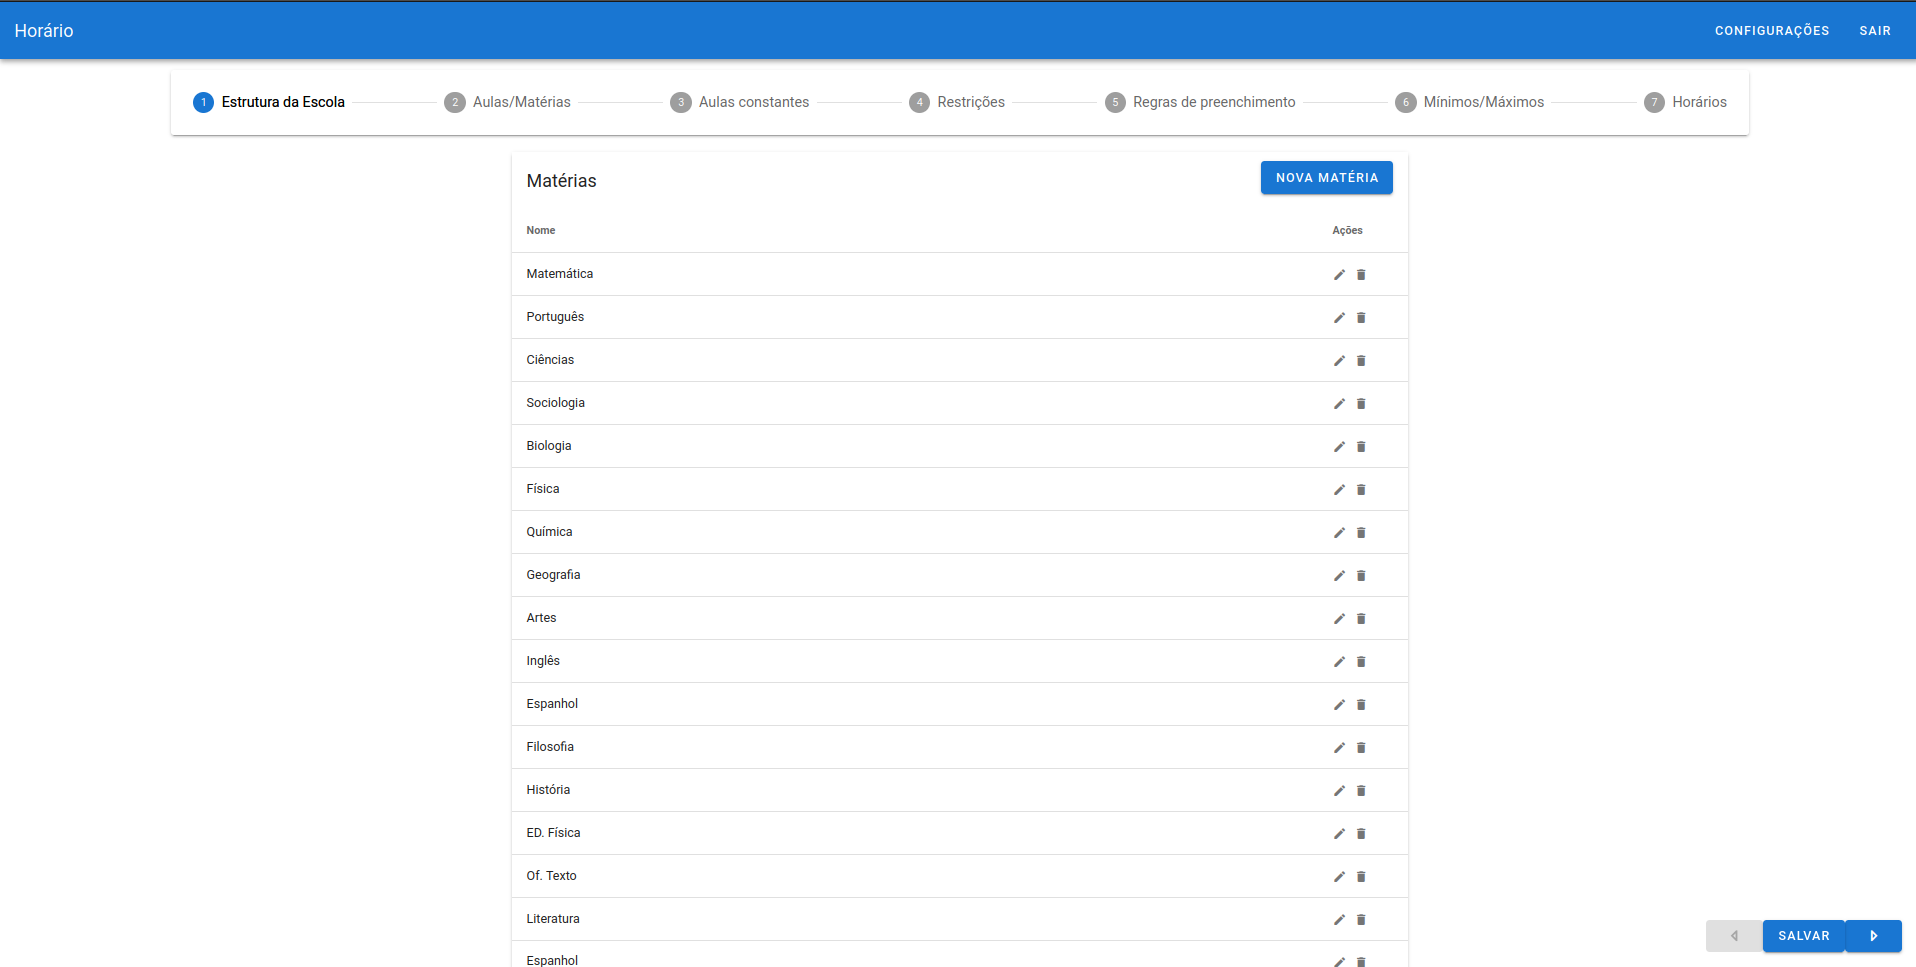
\includegraphics[width=0.65\textwidth]{./dados/figuras/alteracaoEstrutura}
	\fonte{Autor}
	\label{fig:estruturaAtualizada}
\end{figure}
\pagebreak

Além da tela de estrutura, a segunda aba da configuração ("Aulas/Matérias") foi alterada para que fosse possível vincular matérias aos professores, e configurar a quantidade de aulas de cada matéria deve ser ministrada semanalmente, conforme a figura \ref{fig:alteracaoAulas}.

\begin{figure}[!htb]
	\centering
	\caption{Tela de configuração de quantidades de aulas por matéria}
	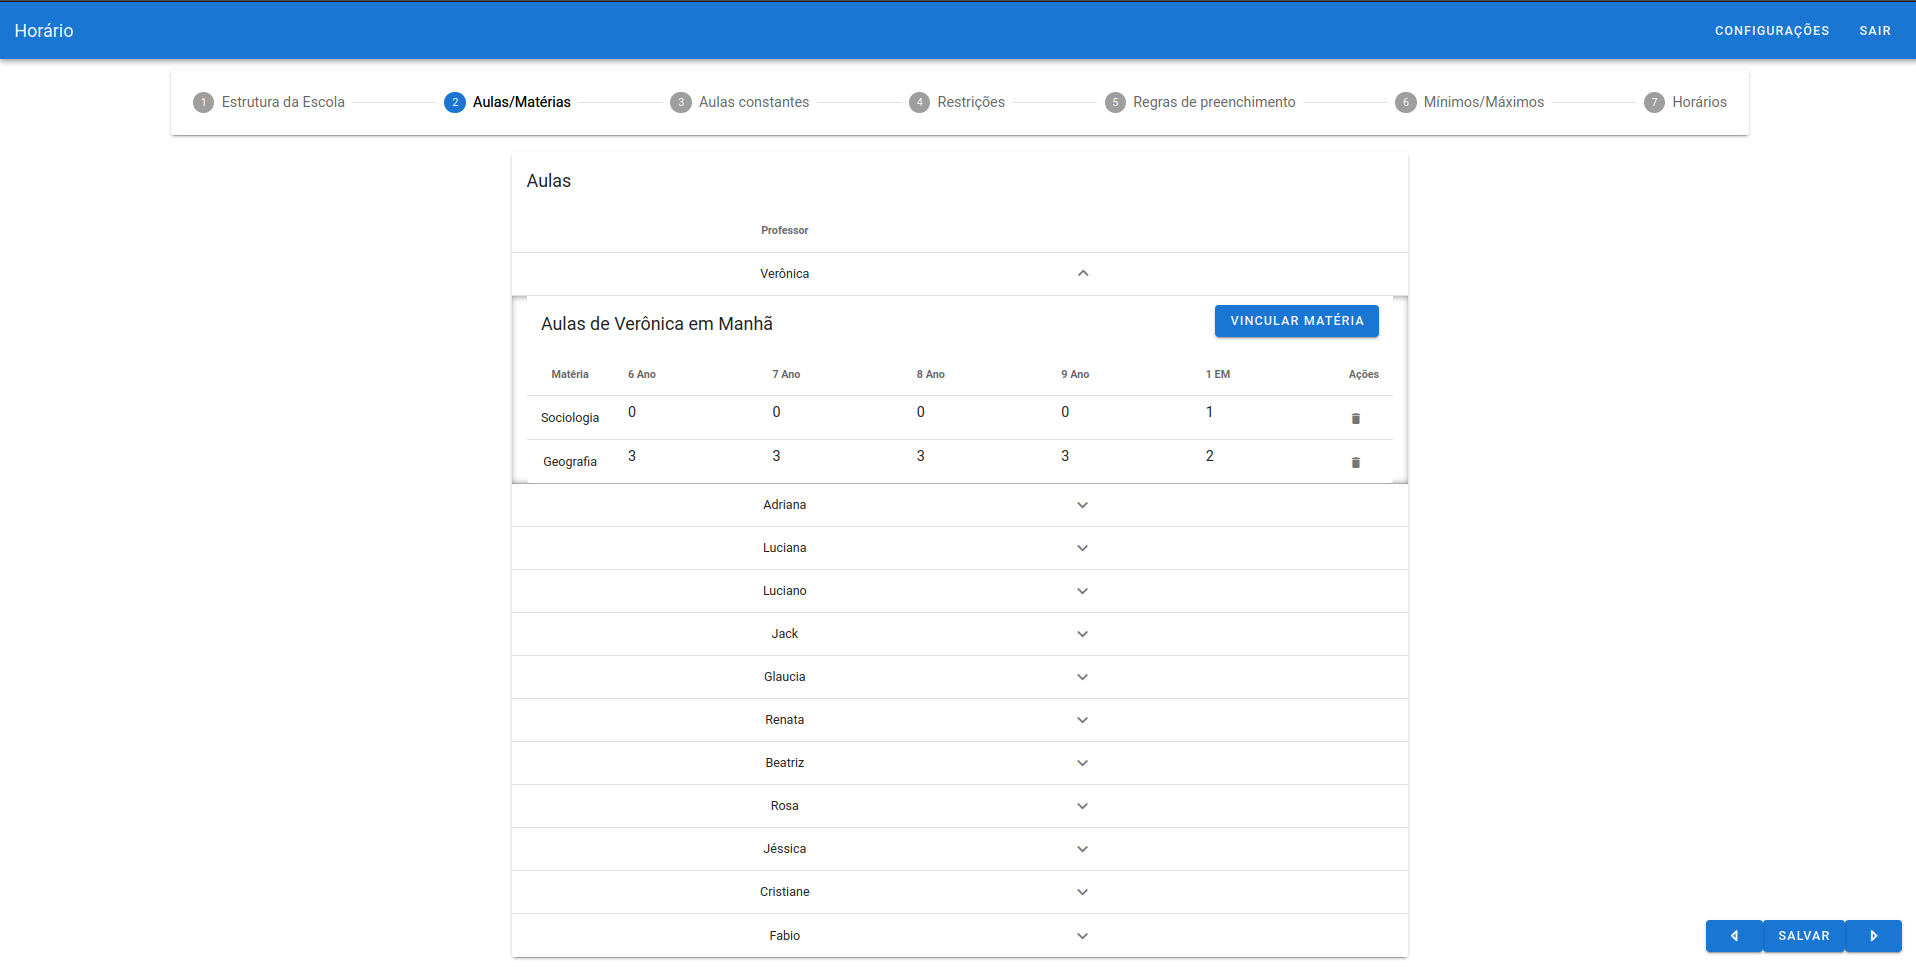
\includegraphics[width=0.65\textwidth]{./dados/figuras/alteracaoAulas}
	\fonte{Autor}
	\label{fig:alteracaoAulas}
\end{figure}

Por fim, na tela final da configuração, representável por exibir as grades horárias geradas, foi necessário alterar o componente da grade para incluir, além dos nomes dos professores, os nomes das matérias alocadas para cada horário, como pode ser visto na figura \ref{fig:alteracaoHorario}.

\begin{figure}[!htb]
	\centering
	\caption{Visualização de grade horária com matérias}
	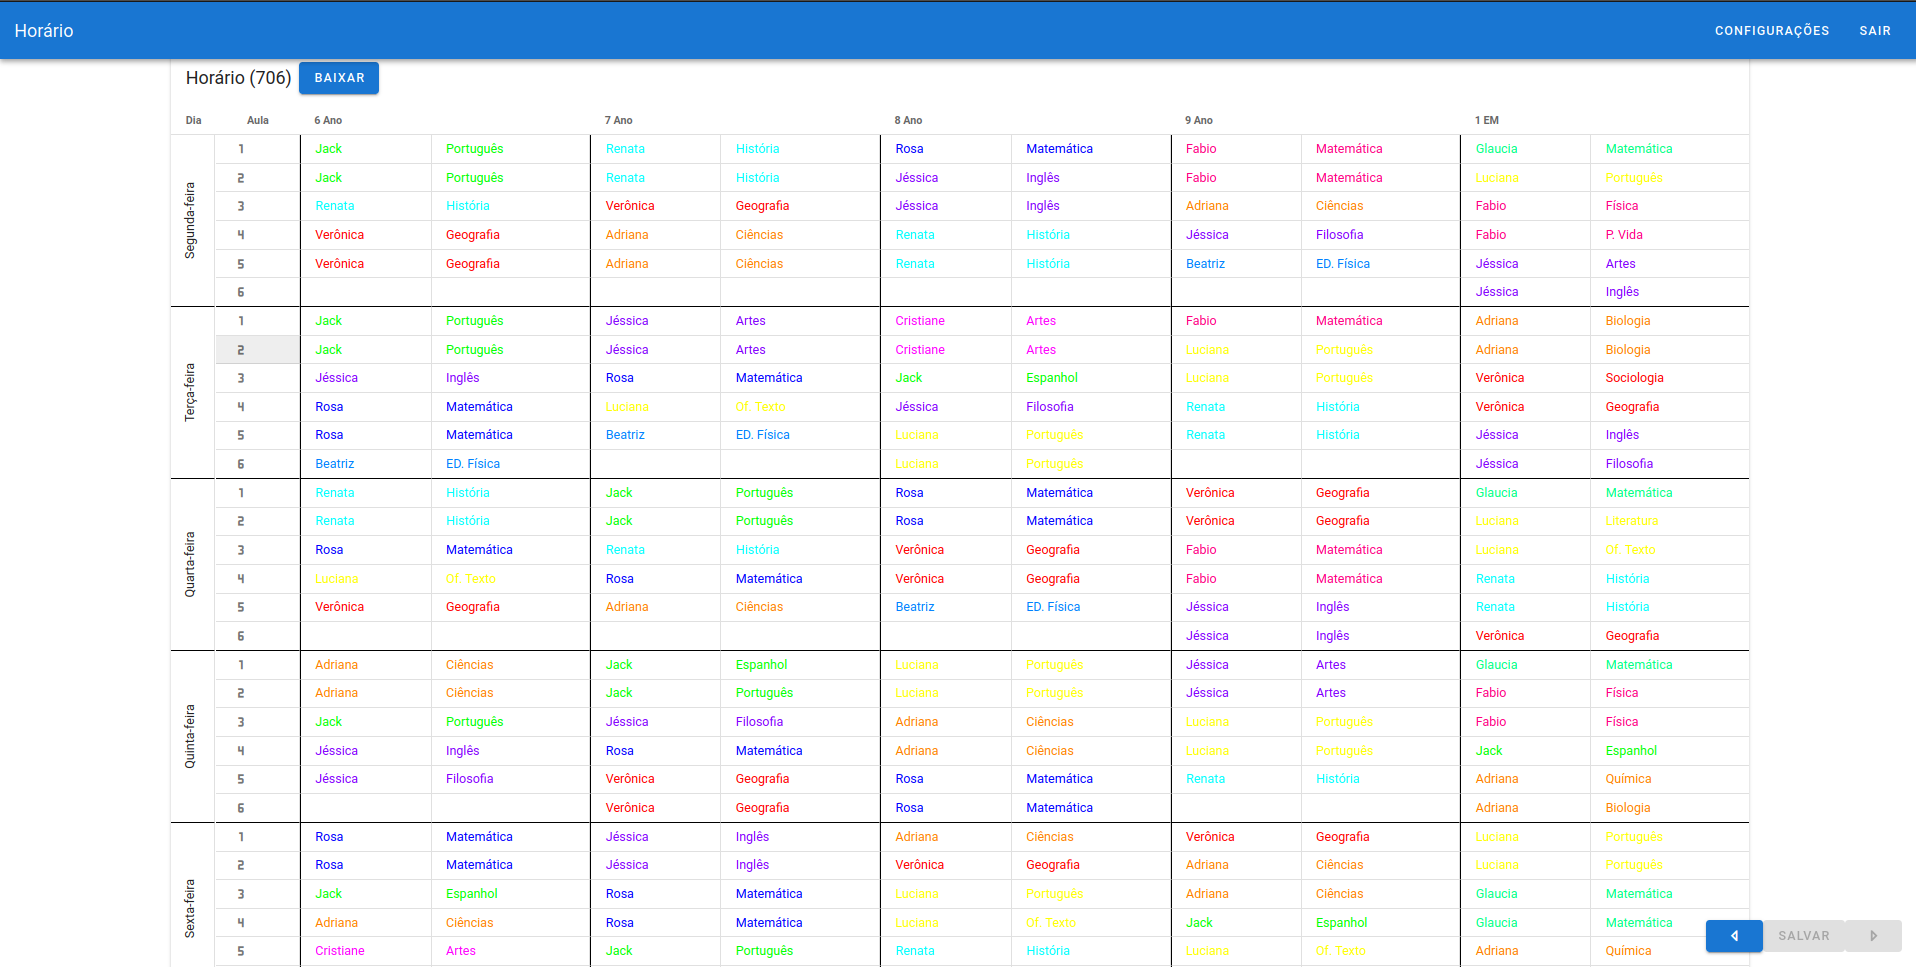
\includegraphics[width=0.65\textwidth]{./dados/figuras/alteracaoHorarios}
	\fonte{Autor}
	\label{fig:alteracaoHorario}
\end{figure}

\subsubsection{Alteração de métodos no servidor}
A adição das matérias também envolveu algumas alterações no servidor. As rotas alteradas para acomodar a melhoria foram rotas de armazenamento e consulta da estrutura da escola, aulas e grades horárias.

Evidentemente, as funções responsáveis por essas rotas precisaram ser modificadas para interagir corretamente com as novas tabelas criadas durante o desenvolvimento deste incremento.

\subsubsection{Matérias no otimizador}
Após as alterações na interface, servidor e banco de dados, o sistema estava pronto para lidar com as informações relacionadas às matérias, faltando apenas a incorporação destas na geração de grades horárias por parte do otimizador. Para realizar isso, implementou-se um método análogo ao \autoref{alg:otimizadorComRestricoes}, porém voltado à geração de grades de matérias.

A diferença é que o novo método implementado obtém determinada grade horária gerada pelo \autoref{alg:otimizadorComRestricoes}, e realiza as operações necessárias para preencher a grade com matérias. Vale ressaltar que essas operações são semelhantes à geração da grade de aulas dos professores: preenchimento da grade inicial, cálculo da variação de custo, realização de trocas de posições e armazenamento das soluções.

O método de geração de grades foi aplicado no otimizador de forma que cada vez que uma grade horária de professores é salva no banco de dados, esta também já tem a sua grade horária de matérias gerada, completando assim o processo de otimização da grade, conforme o \autoref{alg:otimizadorCompleto}.

\begin{algorithm}
	\caption{Otimizador com matérias}
	\label{alg:otimizadorCompleto}
	\KwIn{Lista de professores $LP$, lista de turmas $LT$, matriz de aulas e matérias por professor por turma $MA$, temperatura inicial $TI$, Taxa de resfriamento $TR$}
	\KwOut{Grade horária de matérias e professores otimizada}
	$temperatura \leftarrow TI$\\
	$grade \leftarrow$ CriaGradeInicial$(LP, LT, MA)$\\
	$iteracoesSemAlteracao \leftarrow 0$\\
	$solucoes \leftarrow$ lista vazia\\
	\While {condição de parada não atingida} {
		$deltaTotal \leftarrow 0$\\
		\For {$passo = 0$ até $numeroPassos$} {
			$turma \leftarrow grade.EscolheTurmaAleatoria()$\\
			$linhas \leftarrow grade.EscolheHorariosAleatoriosValidos(sala)$\\
			$delta \leftarrow grade.CalculaDelta(sala, linhas)$\\
			$probabilidade \leftarrow e^{-delta/temperatura}$\\
			$valorAceite \leftarrow Aleatorio(0, 1)$\\
			\If {$delta < 0$ ou $probabilidade \ge valorAceite$} {
				$grade.PermutaProfessores(sala, linha1, linha2)$\\
				$deltaTotal \leftarrow deltaTotal + delta$\\
				\If {grade não existe na lista de soluções} {
					insere grade na lista de soluções\\
					limita lista de soluções às 100 melhores grades\\
				}
			}
		}
		\eIf {$delta = 0$} {
			$iteracoesSemAlteracao \leftarrow iteracoesSemAlteracao + 1$\\
		}{
			$iteracoesSemAlteracao \leftarrow 0$\\
		}
		\If {$iteracoesSemAlteracao \ge 15$} {
			\For{gradeProfessores em EscolherGradesRelevantes(solucoes)} {
				SalvaGradeProfessores$(gradeProfessores)$\\
				$gradesMaterias \leftarrow$ GeraGradesMaterias$(gradeProfessores)$\\
				SalvarMelhorGradeMaterias$(gradesMaterias)$\\
			}
			apaga lista de soluções\\
			$temperatura \leftarrow TI$\\
			$iteracoesSemAlteracao \leftarrow 0$\\
		}
		$temperatura \leftarrow temperatura * TR$
	}
\end{algorithm}

\subsection{VALIDAÇÃO DE CONFIGURAÇÕES}

Devido à grade quantidade de configurações necessárias para parametrizar a geração de uma grade horária, erros de configurações por parte dos usuários são inevitáveis. Tendo isto em mente, implementou-se uma seção de cótigo no otimizador, responsável pela validação das informações providenciadas pelo usuário.

Vale ressaltar que esta validação não garante que é possível gerar uma grade horária de acordo com as configurações providas, mas ela deve evitar alguns dos erros mais comuns. As validações realizadas foram:

\begin{enumerate}
	\item O total de aulas configurado para cada sala deve ser correto, de acordo com o número de dias da grade horária e quantidade de aulas por dia;
	\item Para cada sala, nenhum professor pode ter mais aulas agendadas do que a sala acomoda;
	\item Nenhum professor pode ter mais aulas constantes configuradas do que o seu total de aulas naquela sala;
	\item Não pode haver uma restrição e aula constante para determinado professor na mesma posição da grade horária;
\end{enumerate}

Estas validações são executadas antes do início das otimizações das grades horárias, e caso haja algum erro de configuração, é exibida uma mensagem alertando o usuário, conforme a \autoref{fig:erroValidacao}.

\begin{figure}[!htb]
	\centering
	\caption{Mensagem de erro de validação}
	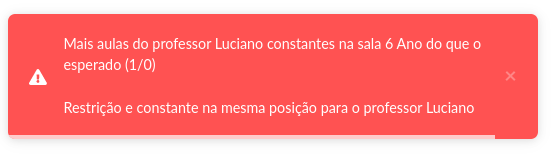
\includegraphics[width=1\textwidth]{./dados/figuras/erroValidacao}
	\fonte{Autor}
	\label{fig:erroValidacao}
\end{figure}
\pagebreak

\section{EXPORTAÇÃO DE GRADES HORÁRIAS}                   % Metodologia
	% RESULTADOS-------------------------------------------------------------------

\chapter{ANÁLISE E DISCUSSÃO DOS RESULTADOS}
\label{chap:resultados}

Este capítulo será responsável por evidenciar o estado final do \textit{software}, trazendo a validação das suas funcionalidades. O capítulo está estruturado em duas seções: a seção \ref{sec:validacao_geral} evidenciará o funcionamento de ponta a ponta geral do sistema, utilizando uma instância arbitrária; enquanto a seção \ref{sec:validacao_datasets} trará os resultados de testes do sistema utilizando alguns \textit{datasets} públicos.

\section{VALIDAÇÃO INTERNA}
\label{sec:validacao_geral}

Conforme amplamente abordado no \autoref{chap:desenvolvimento}, foram desenvolvidos ao longo do projeto três componentes principais: a interface web, a aplicação de servidor e o otimizador de grades. Para validar o funcionamento do sistema como um todo, realizou-se um teste de ponta a ponta, envolvendo os seguintes passos:

\begin{enumerate}
	\item Criar uma nova conta através da interface;
	\item Criar uma nova configuração de grades;
	\item Configurar as quantidades de aulas, e todas as métricas de qualidade;
	\item Requisitar a geração das grades horárias;
	\item Verificar se as configurações foram atendidas corretamente;
	\item Realizar a exportação da grade horária no formato XLSX.
\end{enumerate}

Após a execução dos itens 1 e 2, foi criada uma configuração que foi utilizada para a validação do \textit{software}. Esta configuração de teste contém dois turnos (``Manhã'' e ``Tarde''), cada qual com sete turmas. A tabela \ref{tab:validacao} contém a relação de professores, matérias e turmas do turno da manhã. 

A tabela \ref{tab:validacao} contém o número de aulas que cada professor deve ministrar de cada matéria, em cada uma das turmas. Por exemplo, seguindo esta configuração, a professora ``Adriana'' deve ministrar três aulas de química e três aulas de biologia na turma do ``3º EM''.

\begin{table}[h]
	\centering
	\caption[Configuração de aulas para validação]{Configuração de aulas para validação.
		\label{tab:validacao}}
	\begin{tabular}{rrrrrrrrr}
		\toprule
		Professor & Matéria & 6ºAno & 7ºAno & 8ºAno & 9ºAno & 1ºEM & 2ºEM & 3ºEM \\
		\midrule
		Adriana & Biologia & 0 & 0 & 0 & 0 & 3 & 3 & 3 \\
		Adriana & Ciências & 3 & 3 & 3 & 3 & 0 & 0 & 0 \\
		Adriana & Química & 0 & 0 & 0 & 0 & 3 & 3 & 3 \\
		Beatriz & ED. Física & 1 & 1 & 1 & 1 & 0 & 0 & 0 \\
		Cristiane & Artes & 2 & 0 & 2 & 0 & 0 & 0 & 0 \\
		Fabio & Física & 0 & 0 & 0 & 0 & 3 & 3 & 3 \\
		Fabio & Matemática & 0 & 0 & 0 & 5 & 0 & 0 & 0 \\
		Fabio & P. Vida & 0 & 0 & 0 & 0 & 1 & 1 & 1 \\
		Glaucia & Matemática & 0 & 0 & 0 & 0 & 5 & 5 & 5 \\
		Jack & Espanhol & 1 & 1 & 1 & 1 & 1 & 1 & 1 \\
		Jack & Português & 5 & 5 & 0 & 0 & 0 & 0 & 0 \\
		Jéssica & Artes & 0 & 2 & 0 & 2 & 1 & 1 & 1 \\
		Jéssica & Filosofia & 1 & 1 & 1 & 1 & 1 & 1 & 1 \\
		Jéssica & Inglês & 2 & 2 & 2 & 2 & 2 & 2 & 2 \\
		Luciana & Literatura & 0 & 0 & 0 & 0 & 1 & 1 & 1 \\
		Luciana & Of. Texto & 1 & 1 & 1 & 1 & 1 & 1 & 1 \\
		Luciana & Português & 0 & 0 & 5 & 5 & 3 & 3 & 3 \\
		Renata & História & 3 & 3 & 3 & 3 & 2 & 3 & 2 \\
		Rosa & Matemática & 5 & 5 & 5 & 0 & 0 & 0 & 0 \\
		Verônica & Geografia & 3 & 3 & 3 & 3 & 2 & 2 & 3 \\
		Verônica & Sociologia & 0 & 0 & 0 & 0 & 1 & 0 & 0 \\
		\bottomrule
	\end{tabular}
	\fonte{Autoria própria}
\end{table}


\newpage
Por questão de simplicidade, o turno da tarde contém turmas análogas ao turno da manhã, porém com o sufixo ``B'' para que possam ser diferenciadas. Por exemplo, se no turno da manhã consta a turma ``6º Ano'', no turno da tarde constará a turma ``6º Ano B''.

Para que o teste contemplasse as diversas métricas de qualidade do sistema, configuraram-se também as outras diversas características das grades horárias, que podem ser verificadas nas figuras a seguir. As figuras representam o estado final das interfaces desenvolvidas durante o projeto, e após sua apresentação, constará uma explicação mais detalhada de cada métrica configurada.

\begin{figure}[p]
	\centering
	\caption{Constantes configuradas na interface}
	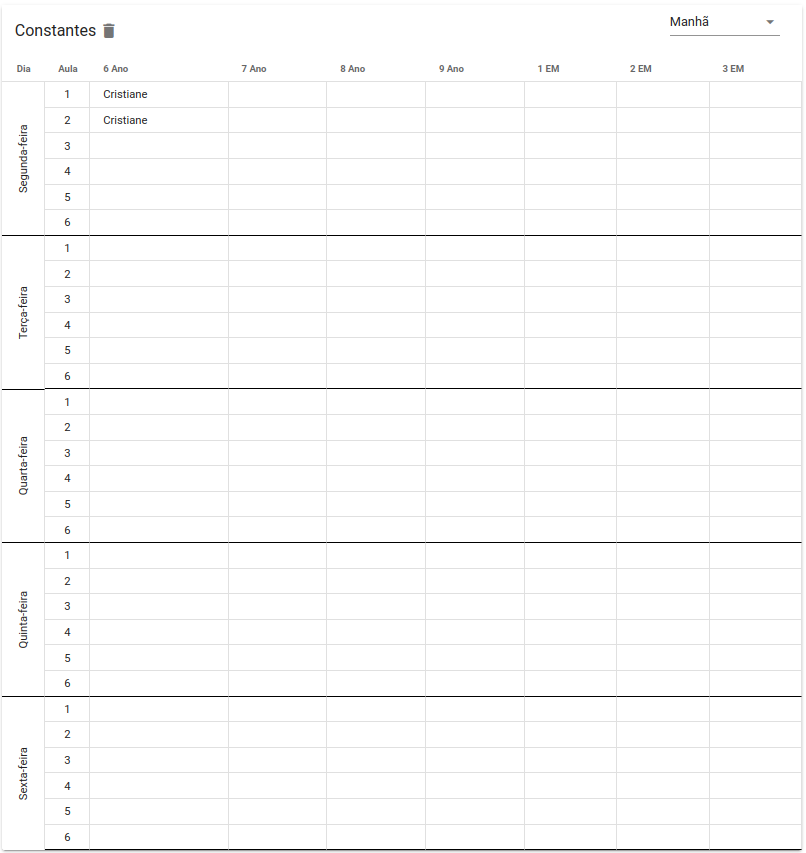
\includegraphics[width=1\textwidth]{./dados/figuras/constantes_configuradas}
	\fonte{Autor}
	\label{fig:constantes_configuradas}
\end{figure}

\begin{figure}[p]
	\centering
	\caption{Restrições e preferências configuradas na interface}
	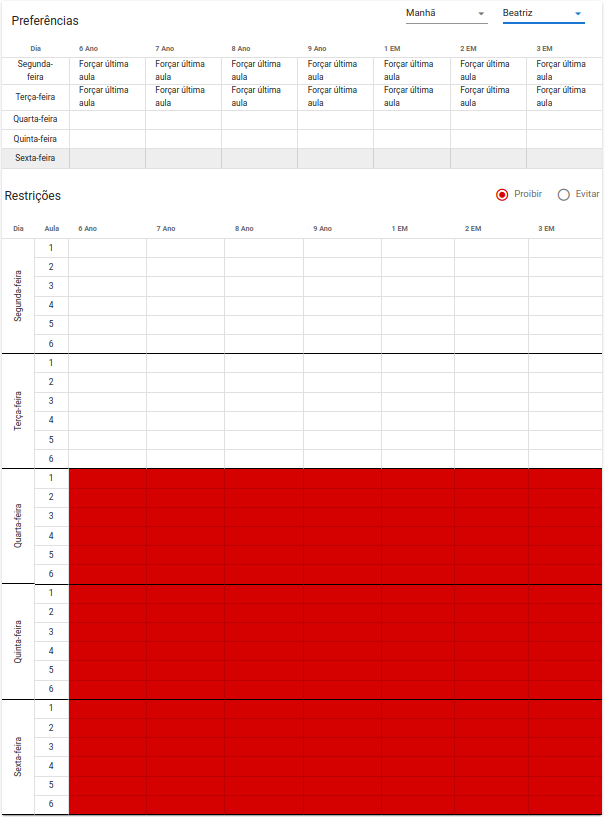
\includegraphics[width=1\textwidth]{./dados/figuras/restricoes_configuradas}
	\fonte{Autor}
	\label{fig:restricoes_configuradas}
\end{figure}

\begin{figure}[p]
	\centering
	\caption{Regiões e grupos de alinhamento configuradas para o turno da ``Manhã''}
	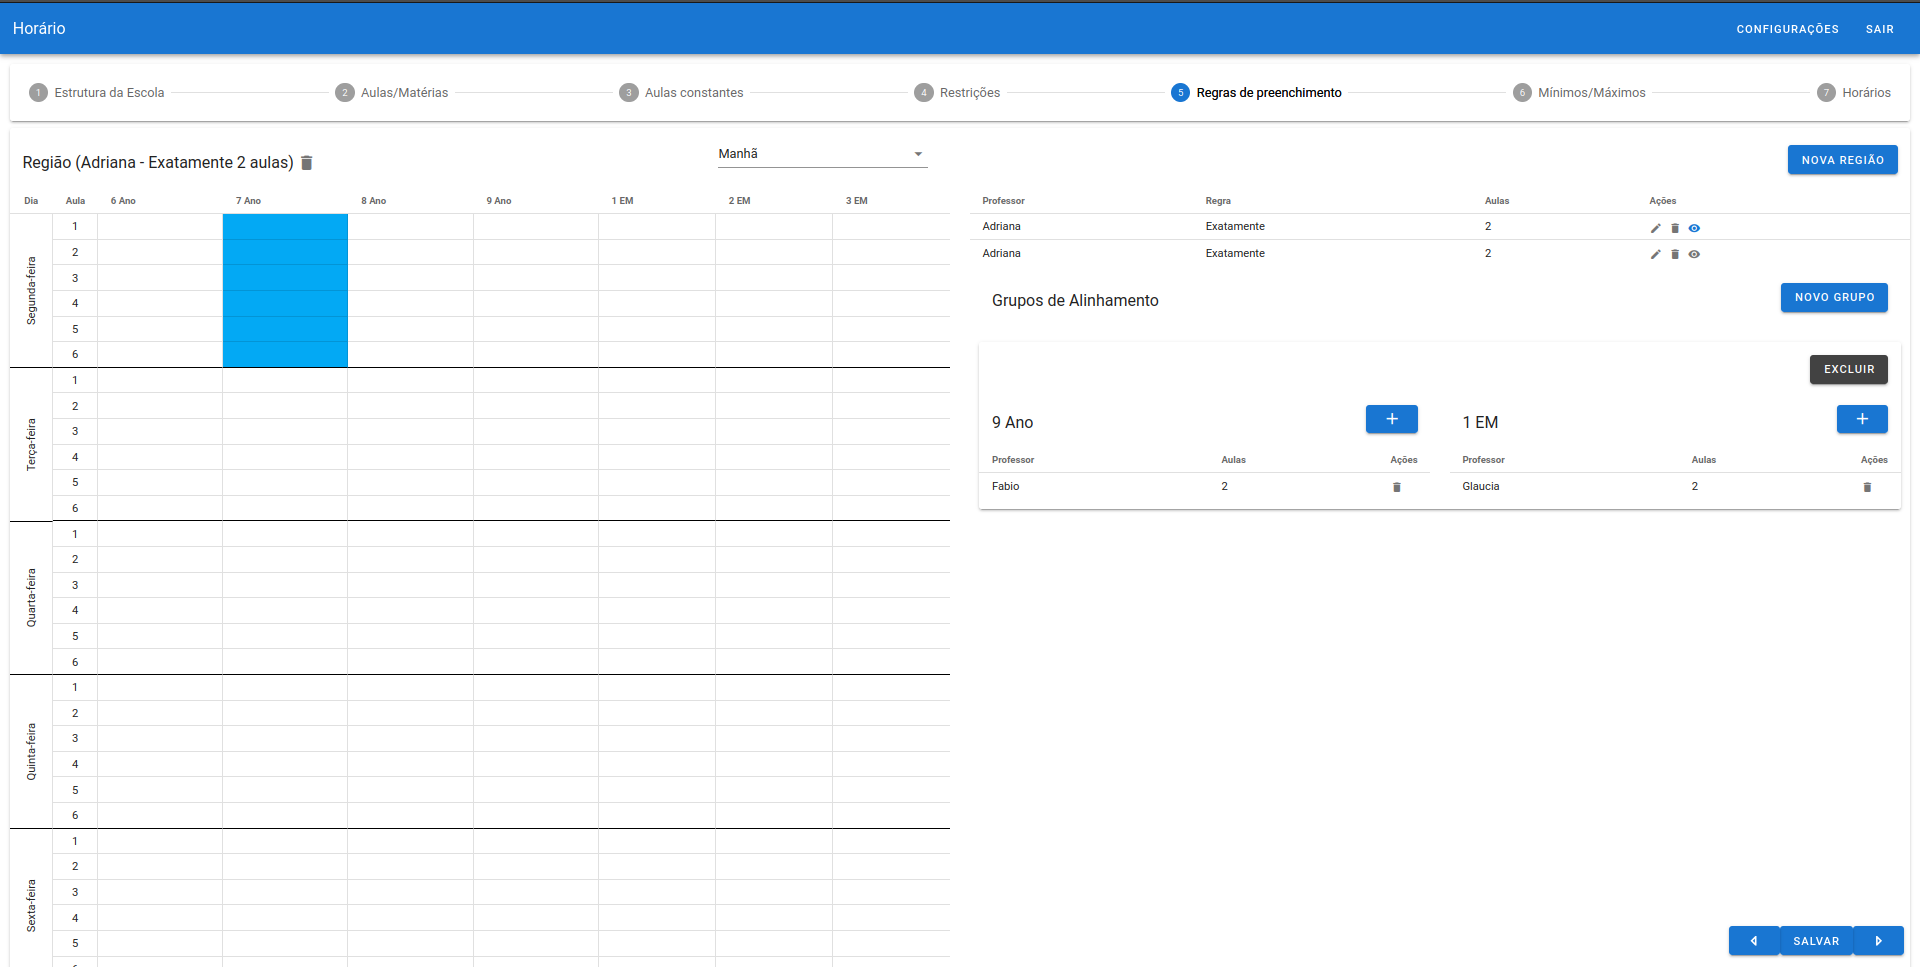
\includegraphics[width=1\textwidth]{./dados/figuras/regioes_configuradas_manha}
	\fonte{Autor}
	\label{fig:regioes_configuradas_manha}
\end{figure}

\begin{figure}[p]
	\centering
	\caption{Regiões e grupos de alinhamento configuradas para o turno da ``Tarde''}
	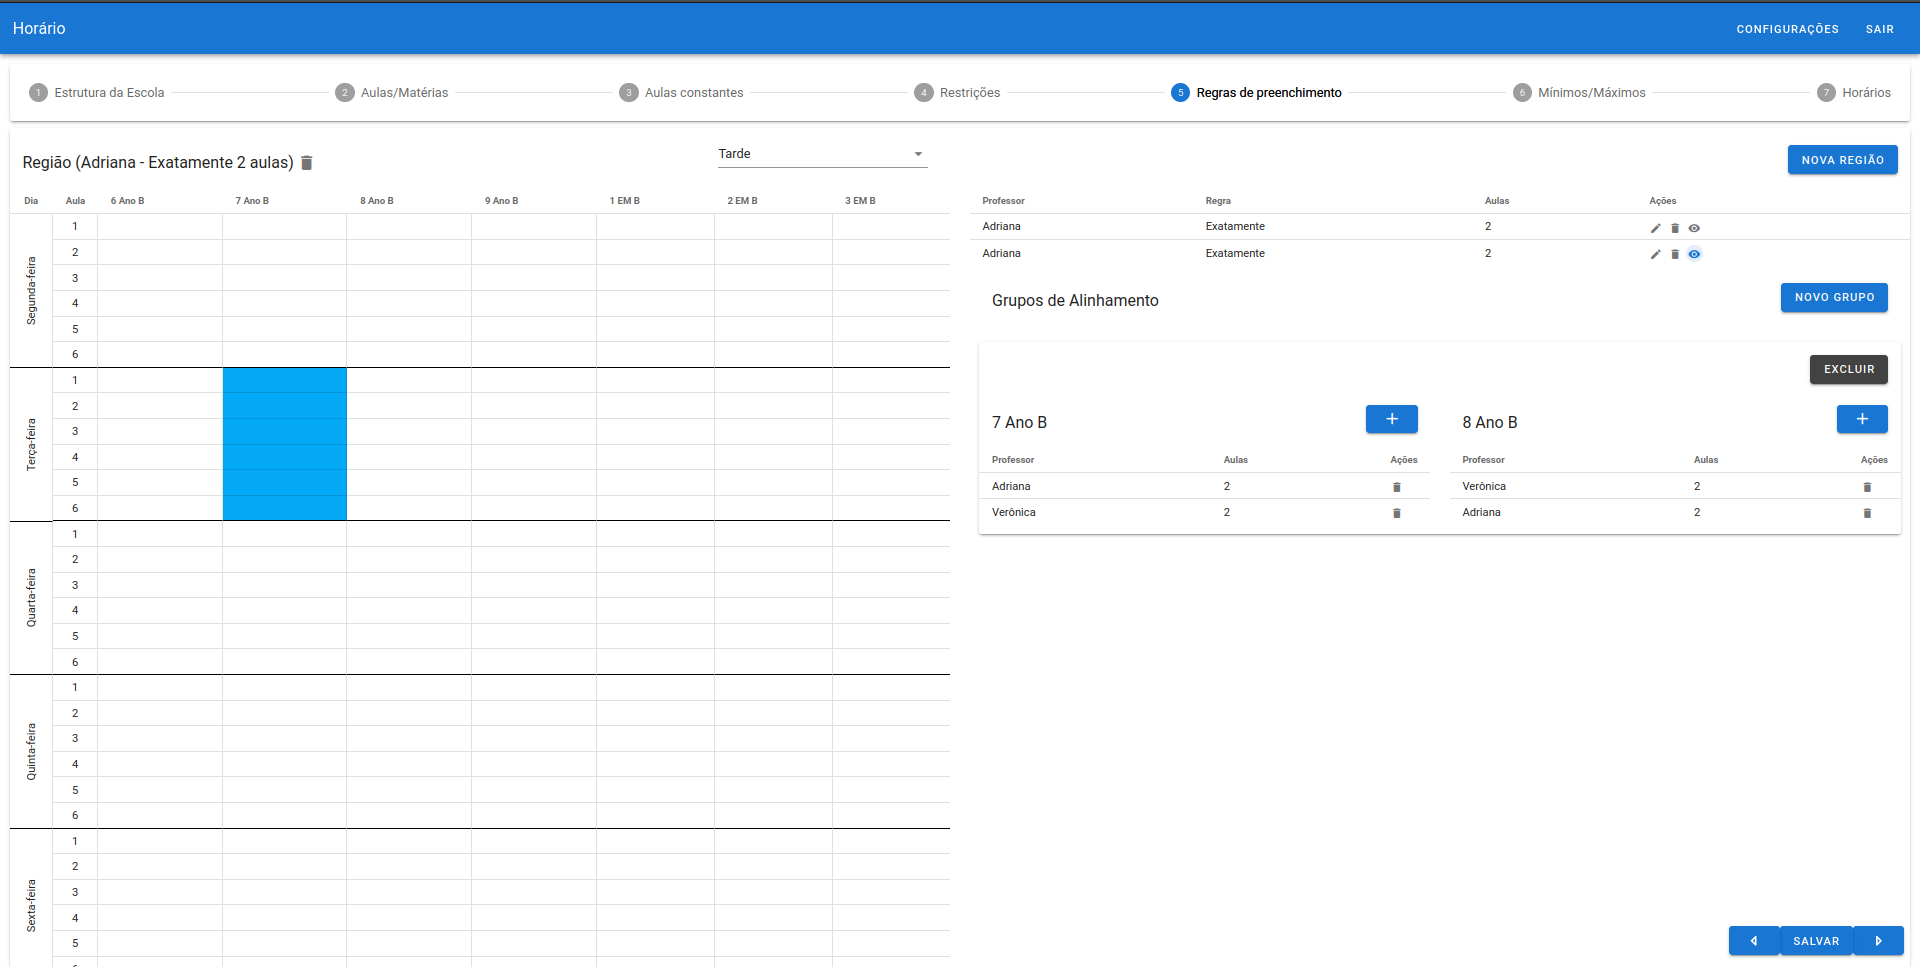
\includegraphics[width=1\textwidth]{./dados/figuras/regioes_configuradas_tarde}
	\fonte{Autor}
	\label{fig:regioes_configuradas_tarde}
\end{figure}

\begin{figure}[h]
	\centering
	\caption{Mínimos de aulas configuradas na interface}
	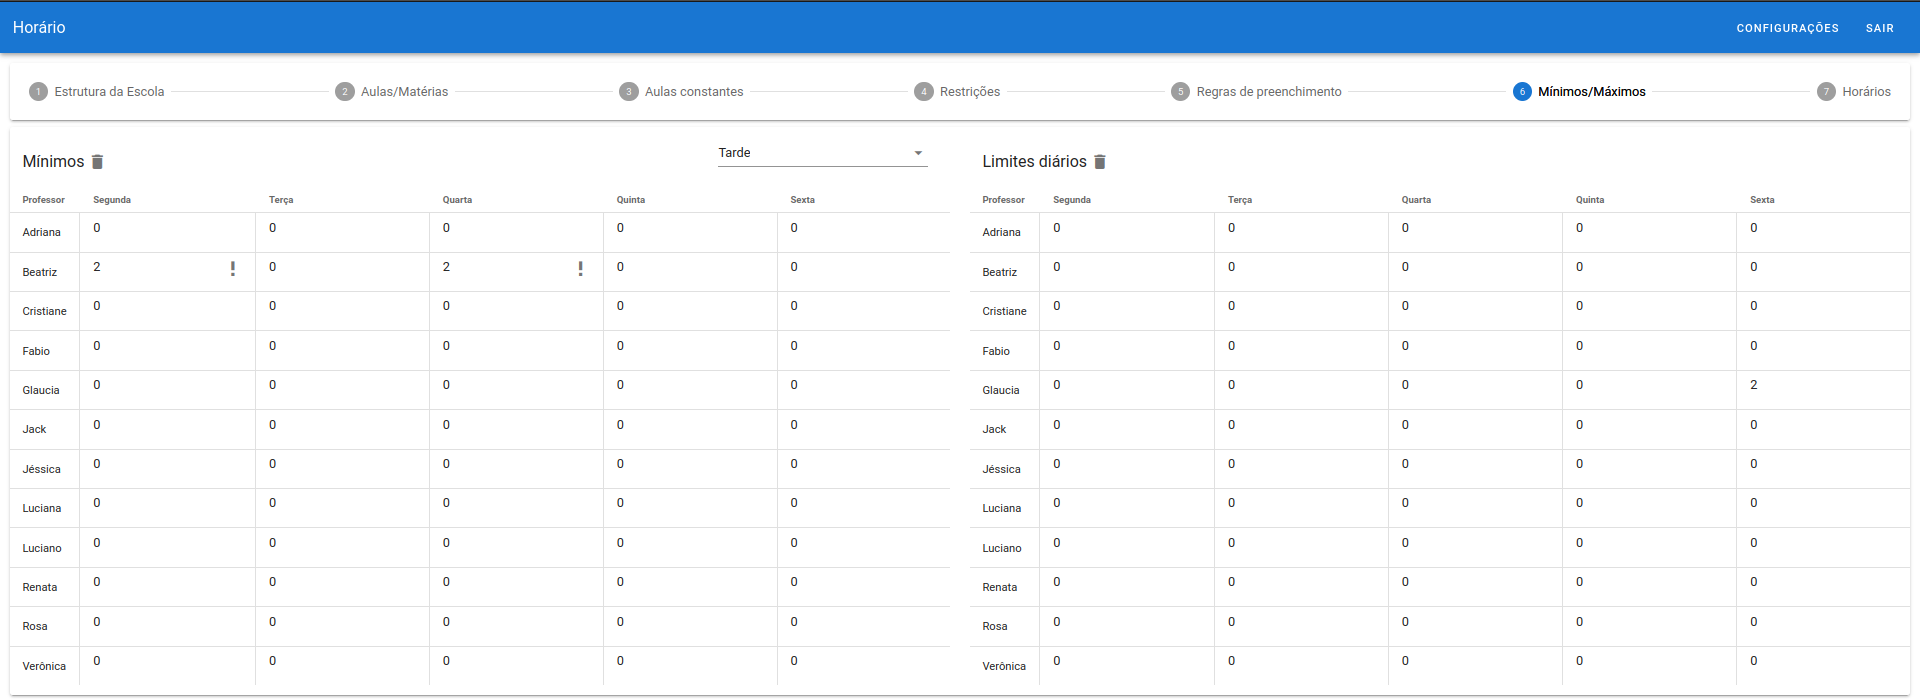
\includegraphics[width=1\textwidth]{./dados/figuras/minimos_configurados}
	\fonte{Autor}
	\label{fig:minimos_configurados}
\end{figure}

\newpage
\begin{enumerate}
	\item \label{item_constantes} \textbf{Constantes}: Conforme a figura \ref{fig:constantes_configuradas}, definiu-se que ``Cristiane'' deveria lecionar as duas primeiras aulas da segunda-feira na turma do ``6º Ano'', em ambos os turnos;
	\item \label{item_restricoes} \textbf{Restrições e preferências}: Na figura \ref{fig:restricoes_configuradas}, é possível notar que no turno da manhã, ``Beatriz'' não deve ter aulas alocadas na quarta, quinta ou sexta-feira. Além disso, informou-se pela interface que suas aulas devem ser lecionadas obrigatoriamente como a última aula do expediente de cada turma;
	\item \label{item_regioes} \textbf{Regiões}: Utilizando o conceito das regiões, definiu-se que ``Adriana'' deveria lecionar exatamente duas aulas para a turma do ``7º Ano'' na segunda-feira, e exatamente 2 aulas para ``7º Ano B'' na terça-feira. Estas configurações abrangem tanto o turno da ``Manhã'', quanto da ``Tarde'', como pode ser visto nas figuras \ref{fig:regioes_configuradas_manha} e \ref{fig:regioes_configuradas_tarde};
	\item \label{item_grupos} \textbf{Grupos de alinhamento}: Definiu-se que duas aulas do professor ``Fábio'' no ``9º Ano'' devem ser alocadas simultaneamente a duas aulas da professora ``Glaucia'' no ``1º EM''. Além disso, duas aulas de ``Adriana'' no ``7º Ano B'' devem ser alocadas simultaneamente a duas aulas de ``Verônica'' no ``8º Ano B'', e vice-versa. Assim como as regiões, as configurações dos grupos de alinhamento podem ser conferidas nas figuras \ref{fig:regioes_configuradas_manha} e \ref{fig:regioes_configuradas_tarde};
	\item \label{item_minimos} \textbf{Mínimos e limites diários}: Como pode ser visto na figura \ref{fig:minimos_configurados}, configurou-se que no turno da tarde, ``Beatriz'' deve ministrar no mínimo duas aulas na segunda-feira e 2 aulas na quarta-feira; além disso, ``Gláucia'' deve ministrar no máximo duas aulas na sexta-feira, contabilizando ambos os turnos.
\end{enumerate}

Realizadas as configurações, o otimizador foi ativado, e utilizou-se como condição de parada a passagem de um intervalo de tempo de um minuto. Durante este intervalo, o otimizador produziu 65 soluções plausíveis diferentes, cada qual contendo uma grade horária para o turno da manhã e uma para o turno da tarde.

\begin{figure}[p]
	\centering
	\caption{Visualização de turno da manhã da melhor solução}
	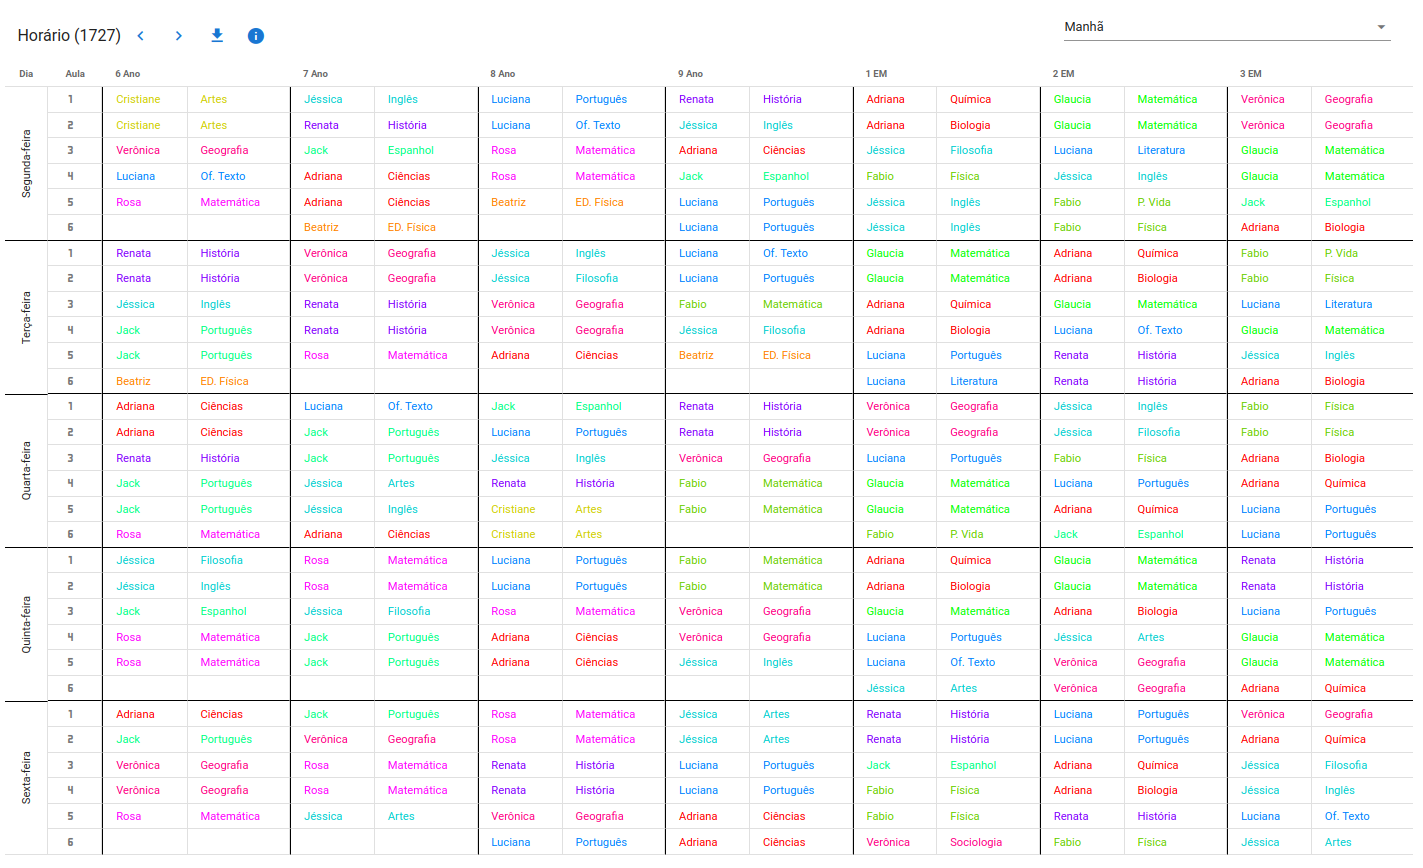
\includegraphics[width=1\textwidth]{./dados/figuras/horario_exportado_manha}
	\fonte{Autor}
	\label{fig:horario_exportado_manha}
\end{figure}

Destas soluções, a melhor encontrada pode ser vista na figura \ref{fig:horario_exportado_manha}, cujas métricas de qualidade foram transcritas para o quadro \ref{qua:caracteristicas_horario_validacao}. Para melhor leitura e análise, as informações de ambos os turnos da grade gerada foram exportadas para as planilhas nas figuras \ref{fig:planilha_exportada_manha} e \ref{fig:planilha_exportada_tarde}, respectivamente.

\begin{quadro}[p]
	\centering
	\caption{Métricas de qualidade da melhor solução.\label{qua:caracteristicas_horario_validacao}}
	\begin{tabular}{|p{8cm}|p{1cm}|p{3cm}|}
		\hline
		\textbf{Nome} & \textbf{Valor} & \textbf{Tipo} \\
		\hline
		Excessos de matérias iguais & 0 & Rígida \\
		\hline
		Restrições violadas & 0 & Rígida \\
		\hline
		Limites diários violados & 0 & Rígida \\
		\hline
		Aulas em grupos de alinhamento não alinhadas & 0 & Rígida \\
		\hline
		Mínimos opcionais violados & 0 & Rígida \\
		\hline
		Mínimos violados & 0 & Rígida \\
		\hline
		Erros nas regiões & 0 & Rígida \\
		\hline
		Matérias desagrupadas & 0 & Rígida \\
		\hline
		Conflitos & 0 & Rígida \\
		\hline
		Aulas desagrupadas & 0 & Rígida \\
		\hline
		Excessos de aulas iguais & 0 & Rígida \\
		\hline
		Dias com todos professores diferentes & 0 & Rígida \\
		\hline
		Restrições opcionais violadas & 0 & Suave \\
		\hline
		Horários com janela (total de todos professores) & 1 & Suave \\
		\hline
		Número de grupos de alinhamento formados & 4 & Suave \\
		\hline
		Preferências não resolvidas & 0 & Suave \\
		\hline
		Aulas separadas & 142 & Suave \\
		\hline
		Dias de professores sem aulas duplas & 0 & Suave \\
		\hline
		Matérias separadas & 208 & Suave \\
		\hline
	\end{tabular}
	\fonte{Autoria própria}
\end{quadro}

\begin{figure}[p]
	\centering
	\caption{Grade exportada - Turno da Manhã}
	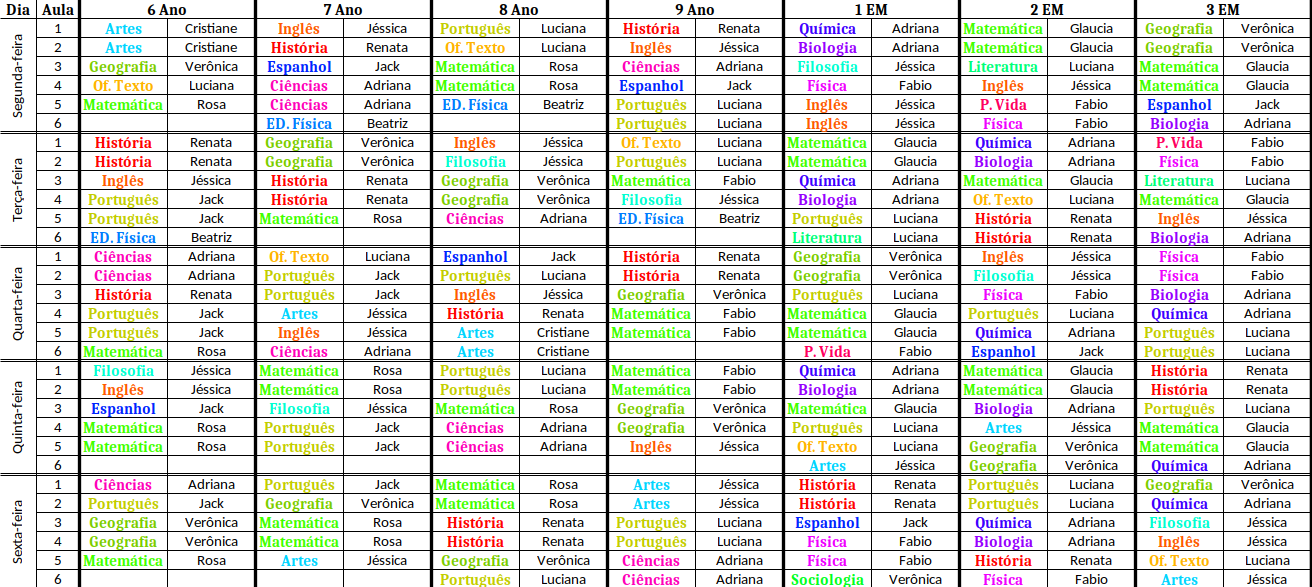
\includegraphics[width=1\textwidth]{./dados/figuras/planilha_exportada_manha}
	\fonte{Autor}
	\label{fig:planilha_exportada_manha}
\end{figure}

\begin{figure}[p]
	\centering
	\caption{Grade exportada - Turno da Tarde}
	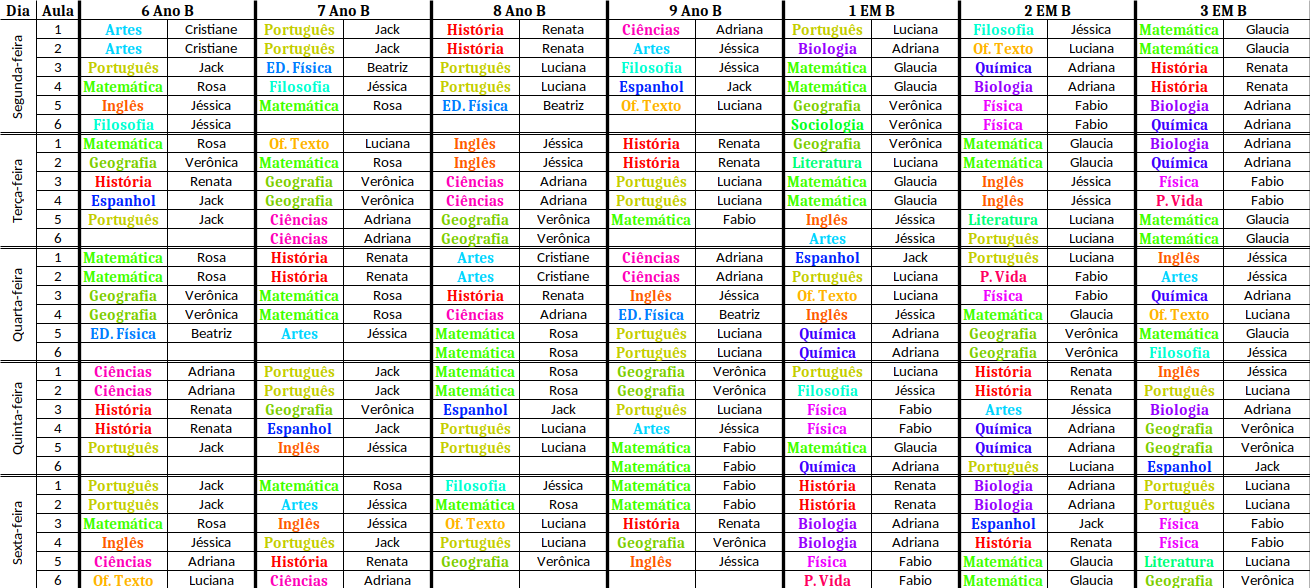
\includegraphics[width=1\textwidth]{./dados/figuras/planilha_exportada_tarde}
	\fonte{Autor}
	\label{fig:planilha_exportada_tarde}
\end{figure}

\newpage
Observando as figuras \ref{fig:planilha_exportada_manha} e \ref{fig:planilha_exportada_tarde}, constata-se que:

\begin{enumerate}
	\item Foi alocada a quantidade correta de aulas para cada professor e matéria, nas turmas corretas, de acordo com a tabela \ref{tab:validacao};
	\item As aulas foram alocadas sem causar conflitos, ou seja, em nenhum horário das grades, um professor está alocado para mais de uma turma simultaneamente;
	\item Aproximadamente 64\% das aulas foram agrupadas: conforme o quadro \ref{qua:caracteristicas_horario_validacao}, apenas 142 do total de 396 aulas permaneceram separadas;
	\item As aulas constantes mencionadas no item \ref{item_constantes} foram alocadas corretamente: Cristiane foi alocada nas duas primeiras aulas da segunda-feira na turma do 6º Ano e 6º Ano B;
	\item As restrições e preferências do item \ref{item_restricoes} foram atendidas: ``Beatriz'' não teve aulas alocadas na quarta, quinta ou sexta-feira no turno da manhã, e neste mesmo turno suas aulas ocuparam sempre os últimos horários do expediente de cada turma;
	\item Em conformidade com o item \ref{item_regioes}, na segunda-feira a professora ``Adriana'' teve exatamente duas aulas alocadas na turma do ``7º Ano'', e duas no ``7º Ano B'';
	\item O grupo de alinhamento da figura \ref{fig:regioes_configuradas_manha} foi respeitado, já que duas aulas do professor ``Fábio'' no ``9º Ano'' foram alocadas simultaneamente a duas aulas de ``Adriana'' no ``1º EM''. As aulas do grupo da figura \ref{fig:regioes_configuradas_tarde} também foram alocadas corretamente;
	\item As quantidades mínimas e máximas de aulas do item \ref{item_minimos} foram respeitadas: foram alocadas para ``Beatriz'' exatamente duas aulas na segunda e quarta-feira no período da tarde; e exatamente duas aulas para ``Gláucia'' na sexta-feira, somando as aulas de ambos os turnos;
\end{enumerate}      


                    % Resultados
	\section{VALIDAÇÃO COM DATASETS PÚBLICOS}
\label{sec:validacao_datasets}

Como visto ao longo deste trabalho, o problema abordado envolve diversos tipos de restrições, tornando trabalhosa a troca de informações entre pesquisadores. Para solucionar esse problema, \citeonline{xhstt} sugeriu o XHSTT, um formato padronizado de arquivo XML para a representação de instâncias e soluções do \textit{High School Timetabling Problem}.

O projeto HSTT da \citeonline{Twente} hospeda publicamente diversas instâncias do problema no formato HXSTT. Destas, selecionaram-se três instâncias brasileiras para complementar a validação do sistema desenvolvido, utilizando dados externos. As próximas subções apresentarão cada instância e os resultados relacionados.

\subsection{Instância 1}

A primeira instância de teste, identificada como ``BrazilInstance1'', é composta por três turmas, 8 professores, cujas aulas devem ser alocadas em uma grade horária de 5 dias por semana, com 5 aulas por dia. As quantidade de aulas por professor em cada turma podem ser conferidas na tabela \ref{tab:config_aulas_br1}.

\begin{table}[h]
	\centering
	\caption[Configuração de Aulas - BrazilInstance1]{Configuração de Aulas - BrazilInstance1.
		\label{tab:config_aulas_br1}}
	\begin{tabular}{rrrrr}
		\toprule
		Professor & Matéria & S1 & S2 & S3 \\
		\midrule
		T1 & M1 & 3 & 3 & 3 \\
		T2 & M2 & 5 & 5 & 0 \\
		T3 & M3 & 3 & 3 & 3 \\
		T4 & M4 & 3 & 3 & 3 \\
		T5 & M5 & 0 & 5 & 5 \\
		T6 & M6 & 4 & 4 & 4 \\
		T7 & M7 & 5 & 0 & 5 \\
		T8 & M8 & 2 & 2 & 2 \\
		\bottomrule
	\end{tabular}
	\fonte{Autoria própria}
\end{table}


Os requisitos associados à instância são:
\begin{enumerate}
	\item Requisito 1 (obrigatório) : Não devem existir conflitos;
	\item Requisito 2 (obrigatório) : Não devem existir janelas;
	\item Requisito 3 (obrigatório) : Cada professor tem um dia da semana específico em que suas aulas não podem ser agendadas;
	\item Requisito 4 (não obrigatório) : Os professores T1, T2, T3, T4. T5, T7 e T8 não devem ser alocados em mais de 2 dias da semana;
	\item Requisito 5 (não obrigatório) : O professor T6 não deve ser alocado em mais de 3 dias da semana;
	\item Requisito 6 (não obrigatório) : Requisitos de quantidades mínimas de aulas duplas, que devido à sua extensão e não obrigatoriedade, não será explicitado.
\end{enumerate}

Sobre o requisito 3, a relação dos dias da semana bloqueados para cada professor pode ser conferida na lista abaixo:
\begin{enumerate}
	\item Segunda-feira: T5;
	\item Terça-feira: T4 e T7;
	\item Quarta-feira: T1 e T6;
	\item Quinta-feira: T3 e T8;
	\item Sexta-feira: T2.
\end{enumerate}

Dado um limite de execução de 10 segundos, o otimizador produziu como melhor solução a grade horária presente na figura \ref{fig:brazilinstance1_solucao}, cujas métricas de qualidade podem ser vistas no quadro \ref{qua:caracteristicas_horario_validacao_brazilinstance1}. Esta solução atende totalmente os requisitos obrigatórios da instância, e atende parcialmente os requisitos não obrigatórios.

\begin{figure}[h]
	\centering
	\caption{Grade exportada - Solução para a instância BrazilInstance1}
	\includegraphics[width=0.5\textwidth]{./dados/figuras/brazilinstance1}
	\fonte{Autor}
	\label{fig:brazilinstance1_solucao}
\end{figure}

\begin{quadro}[h]
	\centering
	\caption{Métricas de qualidade da melhor solução - BrazilInstance1.\label{qua:caracteristicas_horario_validacao_brazilinstance1}}
	\begin{tabular}{|p{8cm}|p{1cm}|p{3cm}|}
		\hline
		\textbf{Nome} & \textbf{Valor} & \textbf{Tipo} \\
		Aulas desagrupadas & 0 & Rígida \\
		\hline
		Aulas em grupos de alinhamento não alinhadas & 0 & Rígida \\
		\hline
		Conflitos & 0 & Rígida \\
		\hline
		Dias com todos professores diferentes & 0 & Rígida \\
		\hline
		Erros nas regiões & 0 & Rígida \\
		\hline
		Excessos de aulas iguais & 0 & Rígida \\
		\hline
		Excessos de matérias iguais & 0 & Rígida \\
		\hline
		Horários com janela (total de todos professores) & 0 & Rígida \\
		\hline
		Limites diários violados & 0 & Rígida \\
		\hline
		Matérias desagrupadas & 0 & Rígida \\
		\hline
		Mínimos opcionais violados & 0 & Rígida \\
		\hline
		Mínimos violados & 0 & Rígida \\
		\hline
		Restrições violadas & 0 & Rígida \\
		\hline
		Excessos de dias trabalhados & 7 & Suave \\
		\hline
		Aulas separadas & 19 & Suave \\
		\hline
		Dias de professores sem aulas duplas & 2 & Suave \\
		\hline
		Matérias separadas & 19 & Suave \\
		\hline
		Número de grupos de alinhamento formados & 0 & Suave \\
		\hline
		Preferências não resolvidas & 0 & Suave \\
		\hline
		Restrições opcionais violadas & 0 & Suave \\
		\hline
	\end{tabular}
	\fonte{Autoria própria}
\end{quadro}

\clearpage
\subsection{Instância 2}

A segunda instância de teste, identificada como ``BrazilInstance5'', é composta por 13 turmas, 31 professores, cujas aulas devem ser alocadas em uma grade horária de 5 dias por semana, com 5 aulas por dia. As quantidade de aulas por professor em cada turma podem ser conferidas na tabela quadro \ref{tab:config_aulas_br5}.

\begin{table}[h]
	\centering
	\caption[Configuração de Aulas - BrazilInstance5]{Configuração de Aulas - BrazilInstance5.
		\label{tab:config_aulas_br5}}
	\begin{tabular}{rrrrrrrrrrrrrrr}
		\toprule
		Professor & Matéria & S1 & S2 & S3 & S4 & S5 & S6 & S7 & S8 & S9 & S 10 & S11 & S12 & S13 \\
		\midrule
		T1 & M1 & 6 & 6 & 6 & 0 & 0 & 0 & 0 & 0 & 0 & 0 & 0 & 0 & 0 \\
		T2 & M2 & 0 & 0 & 0 & 3 & 3 & 3 & 3 & 3 & 3 & 3 & 3 & 0 & 0 \\
		T3 & M3 & 0 & 0 & 0 & 0 & 0 & 0 & 0 & 0 & 0 & 0 & 0 & 3 & 0 \\
		T4 & M4 & 0 & 0 & 0 & 0 & 0 & 0 & 0 & 0 & 0 & 0 & 0 & 0 & 3 \\
		T5 & M5 & 0 & 0 & 0 & 0 & 0 & 0 & 0 & 0 & 0 & 0 & 0 & 2 & 0 \\
		T6 & M6 & 5 & 5 & 5 & 0 & 0 & 0 & 0 & 0 & 0 & 0 & 0 & 0 & 0 \\
		T7 & M7 & 0 & 0 & 0 & 4 & 4 & 4 & 4 & 4 & 0 & 0 & 0 & 0 & 0 \\
		T8 & M8 & 0 & 0 & 0 & 1 & 1 & 1 & 1 & 1 & 5 & 5 & 1 & 4 & 3 \\
		T9 & M9 & 0 & 0 & 0 & 0 & 0 & 0 & 0 & 0 & 0 & 0 & 4 & 0 & 0 \\
		T10 & M10 & 2 & 2 & 2 & 2 & 2 & 2 & 2 & 2 & 2 & 2 & 0 & 2 & 2 \\
		T11 & M11 & 0 & 0 & 0 & 0 & 0 & 0 & 0 & 0 & 0 & 0 & 2 & 0 & 0 \\
		T12 & M12 & 0 & 0 & 0 & 0 & 0 & 0 & 0 & 0 & 0 & 0 & 0 & 0 & 8 \\
		T13 & M13 & 2 & 2 & 2 & 0 & 0 & 0 & 0 & 0 & 0 & 0 & 0 & 0 & 0 \\
		T14 & M14 & 0 & 0 & 0 & 2 & 2 & 2 & 2 & 2 & 0 & 0 & 0 & 0 & 0 \\
		T15 & M15 & 0 & 0 & 0 & 0 & 0 & 0 & 0 & 0 & 2 & 2 & 2 & 2 & 0 \\
		T16 & M16 & 1 & 1 & 1 & 0 & 0 & 0 & 0 & 0 & 0 & 0 & 0 & 0 & 0 \\
		T17 & M17 & 3 & 3 & 3 & 0 & 0 & 0 & 0 & 0 & 0 & 0 & 0 & 0 & 0 \\
		T18 & M18 & 3 & 3 & 3 & 2 & 2 & 0 & 0 & 2 & 0 & 2 & 2 & 0 & 0 \\
		T19 & M19 & 3 & 3 & 3 & 0 & 0 & 2 & 2 & 0 & 2 & 0 & 0 & 2 & 0 \\
		T20 & M20 & 0 & 0 & 0 & 0 & 0 & 0 & 0 & 2 & 0 & 2 & 0 & 0 & 0 \\
		T21 & M21 & 0 & 0 & 0 & 0 & 0 & 0 & 0 & 0 & 2 & 0 & 2 & 2 & 0 \\
		T22 & M22 & 0 & 0 & 0 & 2 & 2 & 2 & 2 & 0 & 0 & 0 & 0 & 0 & 0 \\
		T23 & M23 & 0 & 0 & 0 & 3 & 3 & 3 & 3 & 0 & 0 & 0 & 3 & 0 & 0 \\
		T24 & M24 & 0 & 0 & 0 & 0 & 0 & 0 & 0 & 3 & 3 & 3 & 0 & 0 & 0 \\
		T25 & M25 & 0 & 0 & 0 & 3 & 3 & 3 & 3 & 3 & 3 & 0 & 0 & 0 & 0 \\
		T26 & M26 & 0 & 0 & 0 & 0 & 0 & 0 & 0 & 0 & 0 & 3 & 3 & 2 & 0 \\
		T27 & M27 & 0 & 0 & 0 & 3 & 0 & 0 & 0 & 0 & 0 & 3 & 3 & 0 & 0 \\
		T28 & M28 & 0 & 0 & 0 & 0 & 3 & 3 & 3 & 3 & 3 & 0 & 0 & 3 & 0 \\
		T29 & M29 & 0 & 0 & 0 & 0 & 0 & 0 & 0 & 0 & 0 & 0 & 0 & 0 & 8 \\
		T30 & M30 & 0 & 0 & 0 & 0 & 0 & 0 & 0 & 0 & 0 & 0 & 0 & 1 & 1 \\
		T31 & M31 & 0 & 0 & 0 & 0 & 0 & 0 & 0 & 0 & 0 & 0 & 0 & 2 & 0 \\
		\bottomrule
	\end{tabular}
	\fonte{Autoria própria}
\end{table}


\newpage
Os requisitos associados à instância são:
\begin{enumerate}
	\item Requisito 1 (obrigatório) : Não devem existir conflitos;
	\item Requisito 2 (não obrigatório) : Não devem existir janelas;
	\item Requisito 3 (não obrigatório) : Cada professor tem um l trabalhados por semana, conforme o quadro \ref{qua:limites_dias_trabalhados_brazilinstance5};
	\item Requisito 4 (não obrigatório) : Requisitos de quantidades mínimas de aulas duplas, o qual devido à sua extensão e não obrigatoriedade, não será explicitado.
\end{enumerate}

\begin{quadro}[h]
	\centering
	\caption{Limite de dias trabalhados por professor - BrazilInstance5.\label{qua:limites_dias_trabalhados_brazilinstance5}}
	\begin{tabular}{|p{2cm}|p{4cm}|}
		\hline
		\textbf{Professor} & \textbf{Limite em dias} \\
		\hline
		T1 & 4 \\
		\hline
		T2 & 5 \\
		\hline
		T3 & 2 \\
		\hline
		T4 & 2 \\
		\hline
		T5 & 1 \\
		\hline
		T6 & 3 \\
		\hline
		T7 & 4 \\
		\hline
		T8 & 5 \\
		\hline
		T9 & 2 \\
		\hline
		T10 & 5 \\
		\hline
		T11 & 2 \\
		\hline
		T12 & 4 \\
		\hline
		T13 & 2 \\
		\hline
		T14 & 2 \\
		\hline
		T15 & 2 \\
		\hline
		T16 & 1 \\
		\hline
		T17 & 2 \\
		\hline
		T18 & 4 \\
		\hline
		T19 & 4 \\
		\hline
		T20 & 1 \\
		\hline
		T21 & 2 \\
		\hline
		T22 & 2 \\
		\hline
		T23 & 3 \\
		\hline
		T24 & 2 \\
		\hline
		T25 & 4 \\
		\hline
		T26 & 2 \\
		\hline
		T27 & 2 \\
		\hline
		T28 & 4 \\
		\hline
		T29 & 4 \\
		\hline
		T30 & 1 \\
		\hline
		T31 & 1 \\
		\hline
	\end{tabular}
	\fonte{Autoria própria}
\end{quadro}

Dado um limite de execução de 60 segundos, o otimizador produziu como melhor solução a grade horária presente na figura \ref{fig:brazilinstance5_solucao}, cujas métricas de qualidade podem ser vistas no quadro \ref{qua:caracteristicas_horario_validacao_brazilinstance5}. Esta solução atende totalmente os requisitos 1 e 3, e atende parcialmente os requisitos não obrigatórios 2 e 4.

\begin{figure}[h]
	\centering
	\caption{Grade exportada - Solução para a instância BrazilInstance5}
	\includegraphics[width=1\textwidth]{./dados/figuras/brazilinstance5}
	\fonte{Autor}
	\label{fig:brazilinstance5_solucao}
\end{figure}

\begin{quadro}[h]
	\centering
	\caption{Métricas de qualidade da melhor solução - BrazilInstance5.\label{qua:caracteristicas_horario_validacao_brazilinstance5}}
	\begin{tabular}{|p{8cm}|p{1cm}|p{3cm}|}
		\hline
		\textbf{Nome} & \textbf{Valor} & \textbf{Tipo} \\
		Aulas desagrupadas & 0 & Rígida \\
		\hline
		Aulas em grupos de alinhamento não alinhadas & 0 & Rígida \\
		\hline
		Conflitos & 0 & Rígida \\
		\hline
		Dias com todos professores diferentes & 0 & Rígida \\
		\hline
		Erros nas regiões & 0 & Rígida \\
		\hline
		Excessos de aulas iguais & 0 & Rígida \\
		\hline
		Excessos de matérias iguais & 0 & Rígida \\
		\hline
		Limites diários violados & 0 & Rígida \\
		\hline
		Matérias desagrupadas & 0 & Rígida \\
		\hline
		Mínimos opcionais violados & 0 & Rígida \\
		\hline
		Mínimos violados & 0 & Rígida \\
		\hline
		Restrições violadas & 0 & Rígida \\
		\hline
		Excessos de dias trabalhados & 0 & Suave \\
		\hline
		Horários com janela (total de todos professores) & 11 & Suave \\
		\hline
		Aulas separadas & 99 & Suave \\
		\hline
		Dias de professores sem aulas duplas & 24 & Suave \\
		\hline
		Matérias separadas & 99 & Suave \\
		\hline
		Número de grupos de alinhamento formados & 0 & Suave \\
		\hline
		Preferências não resolvidas & 0 & Suave \\
		\hline
		Restrições opcionais violadas & 0 & Suave \\
		\hline
	\end{tabular}
	\fonte{Autoria própria}
\end{quadro}

\clearpage
\subsection{Instância 3}

A terceira instância de teste, identificada como ``BrazilInstance7'', é composta por 20 turmas, 33 professores, cujas aulas devem ser alocadas em uma grade horária de 5 dias por semana, com 5 aulas por dia. As quantidade de aulas por professor em cada turma podem ser conferidas nas tabelas \ref{tab:config_aulas_br7} e \ref{tab:config_aulas_br7_2}.

\begin{table}[h]
	\centering
	\caption[Configuração de Aulas das turmas S1 a S10 - BrazilInstance7]{Configuração de Aulas - BrazilInstance7.
		\label{tab:config_aulas_br7}}
	\begin{tabular}{rrrrrrrrrrrr}
		\toprule
		Professor & Matéria & S1 & S2 & S3 & S4 & S5 & S6 & S7 & S8 & S9 & S10 \\
		\midrule
		T1 & M1 & 3 & 3 & 3 & 3 & 0 & 0 & 0 & 0 & 0 & 0 \\
		T2 & M2 & 0 & 0 & 0 & 0 & 0 & 0 & 3 & 3 & 3 & 4 \\
		T3 & M3 & 0 & 0 & 0 & 0 & 0 & 0 & 0 & 0 & 0 & 0 \\
		T4 & M4 & 0 & 0 & 0 & 0 & 3 & 3 & 0 & 0 & 0 & 0 \\
		T5 & M5 & 4 & 4 & 4 & 4 & 0 & 0 & 0 & 0 & 0 & 0 \\
		T6 & M6 & 0 & 0 & 0 & 0 & 4 & 4 & 4 & 4 & 0 & 1 \\
		T7 & M7 & 0 & 0 & 0 & 0 & 0 & 0 & 0 & 0 & 4 & 4 \\
		T8 & M8 & 0 & 0 & 0 & 0 & 0 & 0 & 0 & 0 & 0 & 0 \\
		T9 & M9 & 0 & 0 & 0 & 0 & 0 & 0 & 0 & 0 & 0 & 0 \\
		T10 & M10 & 3 & 3 & 3 & 3 & 3 & 0 & 0 & 0 & 0 & 0 \\
		T11 & M11 & 0 & 0 & 0 & 0 & 0 & 3 & 3 & 3 & 3 & 3 \\
		T12 & M12 & 0 & 0 & 0 & 0 & 0 & 0 & 0 & 0 & 0 & 0 \\
		T13 & M13 & 0 & 0 & 0 & 0 & 0 & 0 & 0 & 0 & 0 & 0 \\
		T14 & M14 & 3 & 3 & 3 & 0 & 0 & 0 & 0 & 0 & 0 & 3 \\
		T15 & M15 & 0 & 0 & 0 & 3 & 3 & 3 & 0 & 0 & 0 & 0 \\
		T16 & M16 & 0 & 0 & 0 & 0 & 0 & 0 & 3 & 3 & 3 & 0 \\
		T17 & M17 & 3 & 3 & 3 & 0 & 0 & 0 & 0 & 0 & 0 & 2 \\
		T18 & M18 & 0 & 0 & 0 & 3 & 3 & 3 & 0 & 0 & 0 & 0 \\
		T19 & M19 & 0 & 0 & 0 & 0 & 0 & 0 & 3 & 3 & 3 & 0 \\
		T20 & M20 & 2 & 2 & 2 & 2 & 2 & 2 & 2 & 0 & 0 & 0 \\
		T21 & M21 & 0 & 0 & 0 & 0 & 0 & 0 & 0 & 2 & 2 & 2 \\
		T22 & M22 & 0 & 0 & 0 & 0 & 0 & 0 & 0 & 0 & 0 & 0 \\
		T23 & M23 & 2 & 2 & 2 & 0 & 0 & 0 & 0 & 0 & 0 & 2 \\
		T24 & M24 & 0 & 0 & 0 & 2 & 2 & 2 & 0 & 0 & 0 & 0 \\
		T25 & M25 & 0 & 0 & 0 & 0 & 0 & 0 & 2 & 2 & 2 & 0 \\
		T26 & M26 & 2 & 0 & 0 & 2 & 0 & 0 & 2 & 0 & 0 & 2 \\
		T27 & M27 & 0 & 2 & 0 & 0 & 2 & 0 & 0 & 2 & 0 & 0 \\
		T28 & M28 & 0 & 0 & 2 & 0 & 0 & 2 & 0 & 0 & 2 & 0 \\
		T29 & M29 & 2 & 0 & 0 & 2 & 0 & 0 & 2 & 0 & 0 & 2 \\
		T30 & M30 & 0 & 2 & 0 & 0 & 2 & 0 & 0 & 2 & 0 & 0 \\
		T31 & M31 & 0 & 0 & 2 & 0 & 0 & 2 & 0 & 0 & 2 & 0 \\
		T32 & M32 & 1 & 1 & 1 & 1 & 1 & 1 & 1 & 1 & 1 & 0 \\
		T33 & M33 & 0 & 0 & 0 & 0 & 0 & 0 & 0 & 0 & 0 & 0 \\
		\bottomrule
	\end{tabular}
	\fonte{Dataset hospedado pela Universidade de \citeonline{Twente}}
\end{table}

\begin{table}[h]
	\centering
	\caption[Configuração de Aulas das turmas S11 a S20 - BrazilInstance7]{Configuração de Aulas - BrazilInstance7.
		\label{tab:config_aulas_br7_2}}
	\begin{tabular}{rrrrrrrrrrrr}
		\toprule
		Professor & Matéria & S11 & S12 & S13 & S14 & S15 & S16 & S17 & S18 & S19 & S20 \\
		\midrule
		T1 & M1 & 0 & 0 & 0 & 0 & 0 & 4 & 4 & 0 & 0 & 0 \\
		T2 & M2 & 4 & 0 & 0 & 0 & 0 & 0 & 0 & 0 & 0 & 0 \\
		T3 & M3 & 0 & 4 & 4 & 4 & 4 & 0 & 0 & 0 & 0 & 0 \\
		T4 & M4 & 0 & 0 & 0 & 0 & 0 & 0 & 0 & 4 & 4 & 4 \\
		T5 & M5 & 0 & 0 & 0 & 1 & 0 & 0 & 0 & 0 & 0 & 0 \\
		T6 & M6 & 0 & 1 & 0 & 0 & 0 & 0 & 0 & 0 & 0 & 0 \\
		T7 & M7 & 4 & 4 & 1 & 0 & 0 & 0 & 0 & 0 & 0 & 0 \\
		T8 & M8 & 1 & 0 & 4 & 4 & 4 & 4 & 0 & 0 & 0 & 0 \\
		T9 & M9 & 0 & 0 & 0 & 0 & 1 & 0 & 4 & 4 & 4 & 4 \\
		T10 & M10 & 0 & 0 & 0 & 0 & 0 & 0 & 0 & 0 & 0 & 0 \\
		T11 & M11 & 0 & 0 & 0 & 0 & 0 & 0 & 0 & 0 & 0 & 0 \\
		T12 & M12 & 3 & 3 & 3 & 3 & 3 & 0 & 0 & 0 & 0 & 0 \\
		T13 & M13 & 0 & 0 & 0 & 0 & 0 & 3 & 3 & 3 & 3 & 3 \\
		T14 & M14 & 0 & 0 & 3 & 0 & 0 & 2 & 2 & 0 & 0 & 0 \\
		T15 & M15 & 3 & 0 & 0 & 3 & 0 & 0 & 0 & 2 & 2 & 0 \\
		T16 & M16 & 0 & 3 & 0 & 0 & 3 & 0 & 0 & 0 & 0 & 2 \\
		T17 & M17 & 0 & 0 & 2 & 0 & 0 & 2 & 2 & 0 & 0 & 0 \\
		T18 & M18 & 2 & 0 & 0 & 2 & 0 & 0 & 0 & 2 & 2 & 0 \\
		T19 & M19 & 0 & 2 & 0 & 0 & 2 & 0 & 0 & 0 & 0 & 2 \\
		T20 & M20 & 0 & 0 & 0 & 0 & 0 & 0 & 0 & 0 & 0 & 0 \\
		T21 & M21 & 2 & 2 & 2 & 2 & 0 & 0 & 0 & 0 & 0 & 0 \\
		T22 & M22 & 0 & 0 & 0 & 0 & 2 & 2 & 2 & 2 & 2 & 2 \\
		T23 & M23 & 2 & 2 & 0 & 0 & 0 & 0 & 0 & 0 & 2 & 0 \\
		T24 & M24 & 0 & 0 & 2 & 2 & 2 & 0 & 0 & 0 & 0 & 2 \\
		T25 & M25 & 0 & 0 & 0 & 0 & 0 & 2 & 2 & 2 & 0 & 0 \\
		T26 & M26 & 0 & 0 & 2 & 0 & 0 & 2 & 0 & 0 & 2 & 0 \\
		T27 & M27 & 2 & 0 & 0 & 2 & 0 & 0 & 2 & 0 & 0 & 2 \\
		T28 & M28 & 0 & 2 & 0 & 0 & 2 & 0 & 0 & 2 & 0 & 0 \\
		T29 & M29 & 0 & 0 & 2 & 0 & 0 & 2 & 0 & 0 & 2 & 0 \\
		T30 & M30 & 2 & 0 & 0 & 2 & 0 & 0 & 2 & 0 & 0 & 0 \\
		T31 & M31 & 0 & 2 & 0 & 0 & 2 & 0 & 0 & 2 & 0 & 2 \\
		T32 & M32 & 0 & 0 & 0 & 0 & 0 & 1 & 1 & 1 & 1 & 1 \\
		T33 & M33 & 0 & 0 & 0 & 0 & 0 & 1 & 1 & 1 & 1 & 1 \\
		\bottomrule
	\end{tabular}
	\fonte{Dataset hospedado pela Universidade de \citeonline{Twente}}
\end{table}



\newpage
Os requisitos associados à instância são:
\begin{enumerate}
	\item Requisito 1 (obrigatório) : Não devem existir conflitos;
	\item Requisito 2 (não obrigatório) : Não devem existir janelas;
	\item Requisito 3 (não obrigatório) : Cada professor tem um limite de dias trabalhados por semana, conforme o quadro \ref{qua:limites_dias_trabalhados_brazilinstance7};
	\item Requisito 4 (não obrigatório) : Requisitos de quantidades mínimas de aulas duplas, o qual devido à sua extensão e não obrigatoriedade, não será explicitado.
\end{enumerate}

\begin{quadro}[h]
	\centering
	\caption{Limite de dias trabalhados por professor - BrazilInstance7.\label{qua:limites_dias_trabalhados_brazilinstance7}}
	\begin{tabular}{|p{2cm}|p{4cm}|}
		\hline
		\textbf{Professor} & \textbf{Limite em dias} \\
		\hline
		T1 & 4 \\
		\hline
		T2 & 4 \\
		\hline
		T3 & 4 \\
		\hline
		T4 & 4 \\
		\hline
		T5 & 4 \\
		\hline
		T6 & 4 \\
		\hline
		T7 & 4 \\
		\hline
		T8 & 4 \\
		\hline
		T9 & 4 \\
		\hline
		T10 & 3 \\
		\hline
		T11 & 3 \\
		\hline
		T12 & 3 \\
		\hline
		T13 & 3 \\
		\hline
		T14 & 4 \\
		\hline
		T15 & 4 \\
		\hline
		T16 & 4 \\
		\hline
		T17 & 4 \\
		\hline
		T18 & 4 \\
		\hline
		T19 & 3 \\
		\hline
		T20 & 3 \\
		\hline
		T21 & 3 \\
		\hline
		T22 & 3 \\
		\hline
		T23 & 3 \\
		\hline
		T24 & 3 \\
		\hline
		T25 & 3 \\
		\hline
		T26 & 3 \\
		\hline
		T27 & 3 \\
		\hline
		T28 & 3 \\
		\hline
		T29 & 3 \\
		\hline
		T30 & 3 \\
		\hline
		T31 & 3 \\
		\hline
		T32 & 3 \\
		\hline
		T33 & 1 \\
		\hline
	\end{tabular}
	\fonte{Autoria própria}
\end{quadro}

\newpage
A melhor solução gerada em um intervalo de 60 segundos pode ser vista nas figuras \ref{fig:brazilinstance7_solucao} e \ref{fig:brazilinstance7_solucao_2}. Vale ressaltar que todas as salas da instância pertecem ao mesmo turno, ou seja, apesar de as turmas terem sido separadas em duas figuras para melhor legibilidade, ainda poderiam ocorrer conflitos entre as turmas S1 e S20, por exemplo.

As métricas de qualidade desta solução podem ser observadas no quadro \ref{qua:caracteristicas_horario_validacao_brazilinstance7}, e indicam que foram atendidos totalmente os requisitos 1 e 3, e parcialmente atendidos os requisitos não obrigatórios 2 e 4.

\begin{figure}[h]
	\centering
	\caption{Solução para a instância BrazilInstance7 - Turmas S1 a S10}
	\includegraphics[width=1\textwidth]{./dados/figuras/brazilinstance7}
	\fonte{Autor}
	\label{fig:brazilinstance7_solucao}
\end{figure}

\begin{figure}[h]
	\centering
	\caption{Solução para a instância BrazilInstance7 - Turmas S11 a S20}
	\includegraphics[width=1\textwidth]{./dados/figuras/brazilinstance7}
	\fonte{Autor}
	\label{fig:brazilinstance7_solucao_2}
\end{figure}

\begin{quadro}[h]
	\centering
	\caption{Métricas de qualidade da melhor solução - BrazilInstance7.\label{qua:caracteristicas_horario_validacao_brazilinstance7}}
	\begin{tabular}{|p{8cm}|p{1cm}|p{3cm}|}
		\hline
		\textbf{Nome} & \textbf{Valor} & \textbf{Tipo} \\
		\hline
		Aulas desagrupadas & 0 & Rígida \\
		\hline
		Aulas em grupos de alinhamento não alinhadas & 0 & Rígida \\
		\hline
		Conflitos & 0 & Rígida \\
		\hline
		Dias com todos professores diferentes & 0 & Rígida \\
		\hline
		Erros nas regiões & 0 & Rígida \\
		\hline
		Excessos de aulas iguais & 0 & Rígida \\
		\hline
		Excessos de matérias iguais & 0 & Rígida \\
		\hline
		Limites diários violados & 0 & Rígida \\
		\hline
		Matérias desagrupadas & 0 & Rígida \\
		\hline
		Mínimos opcionais violados & 0 & Rígida \\
		\hline
		Mínimos violados & 0 & Rígida \\
		\hline
		Restrições violadas & 0 & Rígida \\
		\hline
		Excessos de dias trabalhados & 3 & Suave \\
		\hline
		Aulas separadas & 164 & Suave \\
		\hline
		Dias de professores sem aulas duplas & 43 & Suave \\
		\hline
		Horários com janela (total de todos professores) & 20 & Suave \\
		\hline
		Matérias separadas & 164 & Suave \\
		\hline
		Número de grupos de alinhamento formados & 0 & Suave \\
		\hline
		Preferências não resolvidas & 0 & Suave \\
		\hline
		Restrições opcionais violadas & 0 & Suave \\
		\hline
	\end{tabular}
	\fonte{Autoria própria}
\end{quadro} 
	%% ORIENTAÇÕES GERAIS------------------------------------------------------------


% SOBRE AS ILUSTRAÇÕES----------------------------------------------------------
\chapter{SOBRE AS ILUSTRAÇÕES}
\label{chap:apSobreIlust}

A seguir exemplifica-se como inserir ilustrações no corpo do trabalho. As ilustrações serão indexadas automaticamente em suas respectivas listas. A numeração sequencial de figuras, tabelas e equações também ocorre de modo automático.

Referências cruzadas são obtidas através dos comandos \verb|\label{}| e \verb|\ref{}|. Sendo assim, não é necessário por exemplo, saber que o número de certo capítulo é \ref{chap:fundamentacaoTeorica} para colocar o seu número no texto. Outra forma que pode ser utilizada é esta: \autoref{chap:fundamentacaoTeorica}, facilitando a inserção, remoção e manejo de elementos numerados no texto sem a necessidade de renumerar todos esses elementos.

% FIGURAS-----------------------------------------------------------------------
\chapter{FIGURAS}
\label{chap:figuras}

Exemplo de como inserir uma figura. A \autoref{fig:figura-exemplo1} aparece automaticamente na lista de figuras. Para saber mais sobre o uso de imagens no \LaTeX{} consulte literatura especializada \cite{Goossens2007}.

Os arquivos das figuras devem ser armazenados no diretório de "/dados".

\begin{figure}[!htb]
    \centering
    \caption{Exemplo de Figura}
    \includegraphics[width=0.5\textwidth]{./dados/figuras/figura1}
    \fonte{\citeonline{IRL2014}}
    \label{fig:figura-exemplo1}
\end{figure}

% QUADROS E TABELAS---------------------------------------------------------------
\chapter{QUADROS E TABELAS}
\label{chap:tabelas}

Exemplo de como inserir o \autoref{qua:quadro-exemplo1} e a \autoref{tab:tabela-exemplo1}. Ambos aparecem automaticamente nas suas respectivas listas. Para saber mais informações sobre a construção de tabelas no \LaTeX{} consulte literatura especializada \cite{Mittelbach2004}.

Ambos os elementos (Quadros e Tabelas) devem ser criados em arquivos separados para facilitar manutenção e armazenados no diretório de "/dados".

\begin{quadro}[!htb]
    \centering
    \caption{Exemplo de Quadro.\label{qua:quadro-exemplo1}}
    \begin{tabular}{|p{7cm}|p{7cm}|}
        \hline
        \textbf{BD Relacionais} & \textbf{BD Orientados a Objetos} \\
        \hline
        Os dados são passivos, ou seja, certas operações limitadas podem ser automaticamente acionadas quando os dados são usados. Os dados são ativos, ou seja, as solicitações fazem com que os objetos executem seus métodos. & Os processos que usam dados mudam constantemente. \\
        \hline
    \end{tabular}
    \fonte{\citeonline{Barbosa2004}}
\end{quadro}


A diferença entre quadro e tabela está no fato que um quadro é formado por linhas horizontais e verticais. Deve ser utilizado quando o conteúdo é majoritariamente não-numérico. O número do quadro e o título vem acima do quadro, e a fonte, deve vir abaixo. E Uma tabela é formada apenas por linhas verticais. Deve ser utilizada quando o conteúdo é majoritariamente numérico. O número da tabela e o título vem acima da tabela, e a fonte, deve vir abaixo, tal como no quadro.

\begin{table}[!htb]
    \centering
    \caption[Resultado dos testes]{Resultado dos testes.
    \label{tab:tabela-exemplo1}}
    \begin{tabular}{rrrrr}
        \toprule
            & Valores 1 & Valores 2 & Valores 3 & Valores 4 \\
        \midrule
            Caso 1 & 0,86 & 0,77 & 0,81 & 163 \\
            Caso 2 & 0,19 & 0,74 & 0,25 & 180 \\
            Caso 3 & 1,00 & 1,00 & 1,00 & 170 \\
        \bottomrule
    \end{tabular}
    \fonte{\citeonline{Barbosa2004}}
\end{table}


% EQUAÇÕES-----------------------------------------------------------------------
\chapter{EQUAÇÕES}
\label{chap:equacoes}

Exemplo de como inserir a \autoref{eq:equacao-exemplo1} e a Eq. \ref{eq:equacao-exemplo2} no corpo do texto \footnote{Deve-se atentar ao fato de a formatação das equações ficar muito boa esteticamente.}. Observe que foram utilizadas duas formas distintas para referenciar as equações.

\begin{equation}
    X(s) = \int\limits_{t = -\infty}^{\infty} x(t) \, \text{e}^{-st} \, dt
    \label{eq:equacao-exemplo1}
\end{equation}

\begin{equation}
    F(u, v) = \sum_{m = 0}^{M - 1} \sum_{n = 0}^{N - 1} f(m, n) \exp \left[ -j 2 \pi \left( \frac{u m}{M} + \frac{v n}{N} \right) \right]
    \label{eq:equacao-exemplo2}
\end{equation}

% ALGORITMOS-----------------------------------------------------------------------
\chapter{ALGORITMOS}
\label{chap:algoritmos}

Exemplo de como inserir um algoritmo. Para inserção de algoritmos utiliza-se o pacote {\ttfamily algorithm2e} que já está devidamente configurado dentro do template.

Os algoritmos devem ser criados em arquivos separados para facilitar manutenção e armazenados no diretório de "/dados".\\
\\

\begin{algorithm}
    \caption{Exemplo de Algoritmo}
    \KwIn{o número $n$ de vértices a remover, grafo original $G(V, E)$}
    \KwOut{grafo reduzido $G'(V,E)$}
    $removidos \leftarrow 0$ \\
    \While {removidos $<$ n } {
        $v \leftarrow$ Random$(1, ..., k) \in V$ \\
            \For {$u \in adjacentes(v)$} {
                remove aresta (u, v)\\
                $removidos \leftarrow removidos + 1$\\
            }
            \If {há  componentes desconectados} {
                remove os componentes desconectados\\
            }
        }
\end{algorithm}


% SOBRE AS LISTAS--------------------------------------------------------------------
\chapter{SOBRE AS LISTAS}
\label{chap:apSobreLista}

Para construir listas de "\textit{bullets}"{} ou listas enumeradas, inclusive listas aninhadas, é utilizado o pacote \verb|paralist|.

Exemplo de duas listas não numeradas aninhadas, utilizando o comando \verb|\itemize|. Observe a indentação, bem como a mudança automática do tipo de "\textit{bullet}"{} nas listas aninhadas.

\begin{itemize}
    \item item não numerado 1
    \item item não numerado 2
    \begin{itemize}
        \item subitem não numerado 1
        \item subitem não numerado 2
        \item subitem não numerado 3
    \end{itemize}
    \item item não numerado 3
\end{itemize}

Exemplo de duas listas numeradas aninhadas, utilizando o comando \verb|\enumerate|. Observe a numeração progressiva e indentação das listas aninhadas.

\begin{enumerate}
    \item item numerado 1
    \item item numerado 2
    \begin{enumerate}
        \item subitem numerado 1
        \item subitem numerado 2
        \item subitem numerado 3
    \end{enumerate}
    \item item numerado 3
\end{enumerate}

% SOBRE AS CITAÇÕES E CHAMADAS DE REFERÊNCAS----------------------------------------------
\chapter{SOBRE AS CITAÇÕES E CHAMADAS DE REFERÊNCAS}
\label{chap:apSobreCita}

Citações são trechos de texto ou informações obtidas de materiais consultadss quando da elaboração do trabalho. São utilizadas no texto com o propósito de esclarecer, completar e embasar as ideias do autor. Todas as publicações consultadas e utilizadas (por meio de citações) devem ser listadas, obrigatoriamente, nas referências bibliográficas, para preservar os direitos autorais. São classificadas em citações indiretas e diretas.

% CITAÇÕES INDIRETAS-----------------------------------------------------------------------
\chapter{CITAÇÕES INDIRETAS}
\label{chap:citacoesLivres}

É a transcrição, com suas próprias palavras, das idéias de um autor, mantendo-se o sentido original. A citação indireta é a maneira que o pesquisador tem de ler, compreender e gerar conhecimento a partir do conhecimento de outros autores. Quanto à chamada da referência, ela pode ser feita de duas maneiras distintas, conforme o nome do(s) autor(es) façam parte do seu texto ou não. Exemplo de chamada fazendo parte do texto:\\
\\Enquanto \citeonline{Maturana2003} defendem uma epistemologia baseada na biologia. Para os autores, é necessário rever \ldots.\\

A chamada de referência foi feita com o comando \verb|\citeonline{chave}|, que produzirá a formatação correta.

A segunda forma de fazer uma chamada de referência deve ser utilizada quando se quer evitar uma interrupção na sequência do texto, o que poderia, eventualmente, prejudicar a leitura. Assim, a citação é feita e imediatamente após a obra referenciada deve ser colocada entre parênteses. Porém, neste caso específico, o nome do autor deve vir em caixa alta, seguido do ano da publicação. Exemplo de chamada não fazendo parte do texto:\\
\\Há defensores da epistemologia baseada na biologia que argumentam em favor da necessidade de \ldots \cite{Maturana2003}.\\

Nesse caso a chamada de referência deve ser feita com o comando \verb|\cite{chave}|, que produzirá a formatação correta.

% CITAÇÕES DIRETAS-----------------------------------------------------------------------
\chapter{CITAÇÕES DIRETAS}
\label{chap:citacoesLiterais}

É a transcrição ou cópia de um parágrafo, de uma frase, de parte dela ou de uma expressão, usando exatamente as mesmas palavras adotadas pelo autor do trabalho consultado.

Quanto à chamada da referência, ela pode ser feita de qualquer das duas maneiras já mencionadas nas citações indiretas, conforme o nome do(s) autor(es) façam parte do texto ou não. Há duas maneiras distintas de se fazer uma citação direta, conforme o trecho citado seja longo ou curto.

Quando o trecho citado é longo (4 ou mais linhas) deve-se usar um parágrafo específico para a citação, na forma de um texto recuado (4 cm da margem esquerda), com tamanho de letra menor e espaçamento entrelinhas simples. Exemplo de citação longa:
\\\begin{citacao}
    Desse modo, opera-se uma ruptura decisiva entre a reflexividade filosófica, isto é a possibilidade do sujeito de pensar e de refletir, e a objetividade científica. Encontramo-nos num ponto em que o conhecimento científico está sem consciência. Sem consciência moral, sem consciência reflexiva e também subjetiva. Cada vez mais o desenvolvimento extraordinário do conhecimento científico vai tornar menos praticável a própria possibilidade de reflexão do sujeito sobre a sua pesquisa \cite[p.~28]{Silva2000}.
\end{citacao}

Para fazer a citação longa deve-se utilizar os seguintes comandos:
\begin{verbatim}
\begin{citacao}
<texto da citacao>
\end{citacao}
\end{verbatim}

No exemplo acima, para a chamada da referência o comando \verb|\cite[p.~28]{Silva2000}| foi utilizado, visto que os nomes dos autores não são parte do trecho citado. É necessário também indicar o número da página da obra citada que contém o trecho citado.

Quando o trecho citado é curto (3 ou menos linhas) ele deve inserido diretamente no texto entre aspas. Exemplos de citação curta:\\
\\A epistemologia baseada na biologia parte do princípio de que "assumo que não posso fazer referência a entidades independentes de mim para construir meu explicar" \cite[p.~35]{Maturana2003}.\\
\\A epistemologia baseada na biologia de \citeonline[p.~35]{Maturana2003} parte do princípio de que "assumo que não posso fazer referência a entidades independentes de mim para construir meu explicar".

% DETALHES SOBRE AS CHAMADAS DE REFERÊNCIAS---------------------------------------------------------
\chapter{DETALHES SOBRE AS CHAMADAS DE REFERÊNCIAS}
\label{chap:referUtilizadas}

Outros exemplos de comandos para as chamadas de referências e o resultado produzido por estes:\\
\\\citeonline{Maturana2003} \ \ \  \verb|\citeonline{Maturana2003}|\\
\citeonline{Barbosa2004} \ \ \   \verb|\citeonline{Barbosa2004}|\\
\cite[p.~28]{Silva2000} \ \ \  \verb|\cite[p.~28]{Silva2000}|\\
\citeonline[p.~33]{Silva2000} \ \ \   \verb|\citeonline[p.~33]{v}|\\
\cite[p.~35]{Maturana2003} \ \ \   \verb|\cite[p.~35]{Maturana2003}|\\
\citeonline[p.~35]{Maturana2003} \ \ \   \verb|\citeonline[p.~35]{Maturana2003}|\\
\cite{Barbosa2004,Maturana2003} \ \ \   \verb|\cite{Barbosa2004,Maturana2003}|\\

% SOBRE AS REFERÊNCIAS BIBLIOGRÁFICAS-------------------------------------------------------
\chapter{SOBRE AS REFERÊNCIAS BIBLIOGRÁFICAS}
\label{chap:apSobreRefer}

A bibliografia é feita no padrão \textsc{Bib}\TeX{}. As referências são colocadas em um arquivo separado. Neste template as referências são armazenadas no arquivo "base-referencias.bib".

Existem diversas categorias documentos e materiais componentes da bibliografia. A classe abn\TeX{} define as seguintes categorias (entradas):

\begin{verbatim}
@book
@inbook
@article
@phdthesis
@mastersthesis
@monography
@techreport
@manual
@proceedings
@inproceedings
@journalpart
@booklet
@patent
@unpublished
@misc
\end{verbatim}

Cada categoria (entrada) é formatada pelo pacote \citeonline{abnTeX22014d} de uma forma específica. Algumas entradas foram introduzidas especificamente para atender à norma \citeonline{NBR6023:2002}, são elas: \verb|@monography|, \verb|@journalpart|,\verb|@patent|. As demais entradas são padrão \textsc{Bib}\TeX{}. Para maiores detalhes, refira-se a \citeonline{abnTeX22014d}, \citeonline{abnTeX22014b}, \citeonline{abnTeX22014c}.

% NOTAS DE RODAPÉ--------------------------------------------------------------------------
\chapter{NOTAS DE RODAPÉ}
\label{chap:notasRodape}

As notas de rodapé pode ser classificadas em duas categorias: notas explicativas\footnote{é o tipo mais comum de notas que destacam, explicam e/ou complementam o que foi dito no corpo do texto, como esta nota de rodapé, por exemplo.} e notas de referências. A notas de referências, como o próprio nome ja indica, são utilizadas para colocar referências e/ou chamadas de referências sob certas condições.
                   % Capítulo com Orientações de uso do Template
	% CONCLUSÃO--------------------------------------------------------------------

\chapter{CONCLUSÃO}
\label{chap:conclusao}

O presente trabalho abordou o \textit{High School Timetabling Problem}, e a demanda associada por um software de otimização de grades horárias. Verificou-se durante a revisão de literatura a dificuldade que a tarefa de planejamento de grades horárias representa, e que grande parte das instituições de ensino do país ainda realiza essa tarefa manualmente.

Tal software imaginado foi desenvolvido, aplicando a meta-heurística de \textit{Simulated Annealing}, estudada durante a revisão de literatura. Com essa meta-heurística, foi possível expandir a solução proposta por \citeonline{ABRAMSON}, incorporando diversas métricas de qualidade adicionais, como janelas, restrições, aulas constantes, preferências, agrupamentos, entre outras.

No capítulo \ref{chap:resultados}, foi averiguado o funcionamento do \textit{software} utilizando uma instância arbitrária do problema, e três instâncias disponíveis publicamente. Os relatórios gerados pelo software HSeval mostram que nas instâncias testadas, o otimizador desenvolvido atende totalmente os requisitos obrigatórios, e atende satisfatoriamente os requisitos não obrigatórios, quando comparado com as outras soluções.

Considerando o grau de configuração atingido para as grades horárias, a performance do otimizador e atendimento às métricas de qualidade nas instâncias utilizadas para validação, conclui-se que o \textit{software} desenvolvido atingiu os objetivos propostos neste trabalho.

Quanto às limitações do projeto desenvolvido, temos:
\begin{enumerate}
	\item A inexistência do conceito de salas, ou seja, o sistema assume que cada turma sempre recebe suas aulas na mesma sala, o que não reflete a realidade de grandes instituições de ensino;
	\item O fato de que não foram criadas configurações relacionadas a matérias: conceitos como restrições e aulas constantes são vinculados diretamente aos professores;
	\item Devido à natureza não determinística do \textit{Simulated Annealing}, é impossível determinar de antemão se a configuração desejada pelo usuário é plausível, e é difícil estabelecer uma forma razoável de reportar o progresso de otimização para o usuário.
\end{enumerate}

Em relação a sugestões de trabalhos futuros, sugere-se como atividade de interesse uma melhor integração com o formato XHSTT. Este formato de representação das instâncias e soluções é muito abrangente, logo devemos reconhecer o potencial para sistemas que conseguirem utilizá-lo e possibilitarem uma configuração visual intuitiva a seus usuários.
                 			   % Conclusão
	
	\postextual
	% INSERE ELEMENTOS PÓS-TEXTUAIS
	% REFERÊNCIAS------------------------------------------------------------------

% Carrega o arquivo "base-referencias.bib" e extrai automaticamente as referências citadas

\bibliography{./base-referencias}
\bibliographystyle{abntex2-alf} % Define o estilo ABNT para formatar a lista de referências
% OBSERVAÇÕES------------------------------------------------------------------
% Este arquivo não precisa ser alterado.
           			   % Referências
	%% APÊNDICES--------------------------------------------------------------------

\begin{apendicesenv}
\partapendices

% Primeiro apêndice------------------------------------------------------------
\chapter{Nome do apêndice} % Edite para alterar o título deste apêndice
\label{chap:apendiceA}

Lembre-se que a diferença entre apêndice e anexo diz respeito à autoria do texto e/ou material ali colocado.

Caso o material ou texto suplementar ou complementar seja de sua autoria, então ele deverá ser colocado como um apêndice. Porém, caso a autoria seja de terceiros, então o material ou texto deverá ser colocado como anexo.

Caso seja conveniente, podem ser criados outros apêndices para o seu trabalho acadêmico. Basta recortar e colar este trecho neste mesmo documento. Lembre-se de alterar o "label"{} do apêndice.

Não é aconselhável colocar tudo que é complementar em um único apêndice. Organize os apêndices de modo que, em cada um deles, haja um único tipo de conteúdo. Isso facilita a leitura e compreensão para o leitor do trabalho.

% Novo apêndice----------------------------------------------------------------
\chapter{Nome do outro apêndice}
\label{chap:apendiceB}

conteúdo do novo apêndice

\end{apendicesenv}
             			   % Apêndices
	%% ANEXO------------------------------------------------------------------------

\begin{anexosenv}
\partanexos

% Primeiro anexo---------------------------------------------------------------
\chapter{Nome do anexo}     % edite para alterar o título deste anexo
\label{chap:anexoA}

Lembre-se que a diferença entre apêndice e anexo diz respeito à autoria do texto e/ou material ali colocado.

Caso o material ou texto suplementar ou complementar seja de sua autoria, então ele deverá ser colocado como um apêndice. Porém, caso a autoria seja de terceiros, então o material ou texto deverá ser colocado como anexo.

Caso seja conveniente, podem ser criados outros anexos para o seu trabalho acadêmico. Basta recortar e colar este trecho neste mesmo documento. Lembre-se de alterar o "label"{} do anexo.

Organize seus anexos de modo a que, em cada um deles, haja um único tipo de conteúdo. Isso facilita a leitura e compreensão para o leitor do trabalho. É para ele que você escreve.

% Novo anexo-------------------------------------------------------------------
\chapter{Nome do outro anexo}
\label{chap:anexoB}

conteúdo do outro anexo

\end{anexosenv}
               			   % Anexos
	
\end{document}
